%%%% -*- Mode: LaTeX -*-
%!TEX encoding = UTF-8 Unicode

\documentclass[12pt]{article}

% Language setting
\usepackage[english]{babel}

\usepackage[T1]{fontenc}
\usepackage[utf8]{inputenc}

\usepackage{alltt}
\usepackage{holindex}

% Set page size and margins
\usepackage[letterpaper,top=2cm,bottom=2cm,left=3cm,right=3cm,marginparwidth=1.75cm]{geometry}

% Useful packages
\usepackage{amsmath}
\usepackage{graphicx}
\usepackage[colorlinks=true, allcolors=blue]{hyperref}

\documentclass[a4paper,oneside,cleardoublepage=plain,bibliography=totoc]{scrbook}


\usepackage{xurl}  % For breaking long URLs
\usepackage{amsmath, amssymb, amsthm}  % Math packages
\usepackage{graphicx}  % For including images
\usepackage{tikz}  % For drawing diagrams
\usetikzlibrary{positioning, shapes.geometric, arrows}  % TikZ libraries for advanced drawing

\tikzstyle{startstop} = [rectangle, rounded corners, minimum width=3cm, minimum height=1cm,text centered, draw=black, fill=red!30]
\tikzstyle{process} = [rectangle, minimum width=3cm, minimum height=1cm, text centered, draw=black, fill=orange!30]
\tikzstyle{decision} = [diamond, minimum width=3cm, minimum height=1cm, text centered, draw=black, fill=green!30]
\tikzstyle{arrow} = [thick,->,>=stealth]

\usepackage{datetime}  % For custom date formats
\usepackage{natbib}  % For citation styles
\usepackage{floatrow}  % For better float placement
\floatsetup[table]{capposition=top}  % Forces table captions to appear on top
\usepackage[linesnumbered,ruled,vlined]{algorithm2e}  % For writing algorithms
\usepackage{booktabs}  % For better table formatting
\usepackage{paralist}  % For compact lists
\usepackage{titlesec}  % For custom section titles
\usepackage[standardsections]{scrhack}  % Fixes title section conflicts with scrbook
\usepackage{parskip}  % No paragraph indentation; space between paragraphs

% Finally, load hyperref with your desired options
\usepackage[backref=page]{hyperref}  % Defines styles for references/links
\hypersetup{
    linktocpage,  % Links in the table of contents go to page numbers, not section titles
    colorlinks = true,  % Colors for links instead of boxes
    urlcolor = cyan,  % URL links in cyan
    linkcolor = red,  % Internal links in red
    citecolor = blue  % Citation links in blue
}

% The following makes back references more appealing
\renewcommand*{\backref}[1]{}
\renewcommand*{\backrefalt}[4]{[%
  \ifcase #1 Not cited.%
    \or Cited on page~#2.%
    \else Cited on pages #2.%
  \fi]}


 

% Set your individual data for the title page in the configuration file
% AND DON'T SCREW UP THIS DATA! You should know, for example, whether it's
% an Honours thesis or not, or in which semester it is running.

% Set your name:
%  (Well, your name.)
\newcommand{\AuthorName} {Pascal Bercher}


% Set the title of your work:
%  (Choose an informative and interesting title.)
\newcommand{\ProjectTitle} {Template for Project Reports}


% Set which titlepage layout you prefer. Both provide the exact same
% information, they only differ in design to give you a bit of individuality
%  (change second line accordingly)
\newif\ifStandardTitle % do not delete this part!
\StandardTitletrue     % comment out (or use \StandardTitlefalse)
                       % to switch to an alternative title page layout


% Set the name of your school:
%  (School of Computing, School of Engineering,
%   or School of Cybernetics)
\newcommand{\School} {School of Computing}


% Set the name of your college:
%  (However your College is called.)
\newcommand{\College} {College of Engineering, Computing and Cybernetics (CECC)}


% Set your project points:
%  (6 or 12)
%  can be ignored for Honours theses, since those are always 24 pt anyway
%  and hence set automatically
\newcommand{\ProjectPoints} {6}


% Set whether it's an Honours thesis:
%  (change second line accordingly)
\newif\ifHonoursThesis % do not delete this part!
\HonoursThesistrue     % or \HonoursThesisfalse or comment out


% Set your semester:
%  (S1 or S2 or S1/S2 or S2/S1 or Summer)
\newcommand{\Semester} {S2/S1}


% Set your year:
%  (YYYY or YYYY--YYYY in case of S2/S1)
\newcommand{\Year} {2023--2024}


% Set your degree:
%  (Whatever your degree is called.)
%  (Only required if Honours = true)
\newcommand{\Degree} {Bachelor of Advanced Computing}


% Set your course code and name:
%  (Whatever your course code and name is.)
%  (Only required if Honours = false)
\newcommand{\CourseCode} {COMP1234}
\newcommand{\CourseName} {Course Name}


% Set name of first supervisor:
%   (Whatever her or his name is.)
\newcommand{\FirstSupervisor} {Dr.\ FirstName LastName}


% Set whether there's a second supervisor:
%  (change second line accordingly)
\newif\ifTwoOrMoreSupervisors % do not delete this part!
\TwoOrMoreSupervisorstrue     % or \TwoOrMoreSupervisorsfalse or comment out


% Set name of second supervisor:
%  (Whatever her or his name is.)
%  (Only required if TwoSupervisors = true)
\newcommand{\SecondSupervisor} {%
Dr.\ Second Supervisor
%\\Prof.\ Dr.\ Third Supervisor (if there is any)
%\\Prof.\ Dr.\ Dr.\ Fourth Supervisor (if we need four, five, etc.)
}
                             % to specify data used in the title page

% define your own macros here

\newcommand{\Eff} {\ensuremath{\mathit{eff}}}  % example command without arguments
\newcommand{\Pre} {\ensuremath{\mathit{pre}}}  % (again)

% Note that you can easily specify arguments:
% \newcommand{\someMacro}[2] {Argument 1: #1, Argument 2: #2} % example command with two arguments
% you use it via \someMacro{Hello}{World!}


% the following commands are being provided by the amsthm package
% the first parameter states the new environmet's name that can be
% used (due to this definition here) and the second the name that
% will appear in the PDF document
\theoremstyle{definition}
\newtheorem{definition}{Definition}   % well, a formal definition!
\theoremstyle{plain}
\newtheorem{prop}{Proposition} % like a theorem, but less important or evolved
\newtheorem{lem}{Lemma}        % used within a proof of a theorem
\newtheorem{thm}{Theorem}      % well, a theorem! :) important and evolved
\newtheorem{cor}{Corollary}    % basically either a proposition or theorem,
                               %  but one that follows from another theorem.
% There's a lot you can configure about the appearance. If interested,
% open the manual of amsthm or google for tutorials etc. on that package

% the following add a symbol to the definition environment to make it more
% clear when a definition ends (as there is no difference in fonts!). From:
% https://tex.stackexchange.com/questions/226334/change-a-amsthm-theorem-ending
\newcommand{\xqed}[1]{%
    \leavevmode\unskip\penalty9999 \hbox{}\nobreak\hfill
    \quad\hbox{\ensuremath{#1}}}
\newcommand{\Endofdef}{\xqed{\blacksquare}}
\newenvironment{defn}[1]{%
    \begin{definition}#1}{%
    \Endofdef\end{definition}%
}
                                    % define all your macros here


\begin{document}

\pagenumbering{roman}
%
% This document contains two different definitions of the title page
% which one is chosen is defined in the file configuration.tex
%

% only the title page is centered; all other pages are aligned according to books
\newgeometry{left=2.5cm,right=2.5cm,top=2.5cm}
\thispagestyle{empty}

\newdateformat{monthyeardate}{%
  \monthname[\THEMONTH] \THEYEAR}

\ifStandardTitle % the first style is defined now

\noindent
\begin{minipage}[t]{6cm}%
{\footnotesize%
\raisebox{-\height}{{\bfseries The Australian National University}} \\
~2600 ACT~\textbar~Canberra~\textbar~Australia}
\end{minipage}%
\hfill%
\begin{minipage}[b]{10cm}%
\hfill\raisebox{-\height}{\includegraphics[height=2 cm]{figures/ANU-logos/ANU_Primary_Horizontal_Black.jpg}}
\end{minipage}

\ \\[2em]
\phantom{x} \hfill
\begin{minipage}{58.75 mm}
\raggedright
\bfseries \School\\[.5em]
\mdseries%
\noindent\College
\end{minipage}\\[6 em]
\hfill

\noindent
\parbox{140mm}{\sffamily \bfseries \Huge %
Formalization of AVL Trees in HOL4%
}\\[.75 em]
{--- \ifHonoursThesis Honours \else 24 pt research \fi project (S2 2024)}\\[3 em]

\ifHonoursThesis%
A thesis submitted for the degree\\
\emph{\Degree}\\[3 em]
\else%
A report submitted for the course\\
\emph{\CourseCode, \CourseName}\\[3 em]
\fi

\noindent
{\footnotesize \textbf{By:}}\\
Sineeha Kodwani\\[2em]

\noindent
{\footnotesize \bfseries Supervisors:}\\
{\footnotesize Dr. Chun Tian\\
Prof. Michael Norrish}\\[2 em]
\vfill
{\footnotesize \monthyeardate\today}

\else % the alternative design of the title page

\begin{center}
\ \\[1em]
{\bfseries \Huge Formalization of AVL Trees in HOL4}\\[4em]
%
\ifHonoursThesis%
\Large{A thesis submitted for the degree}\\
\Large{\emph{\Degree}}\\[.5em]
{24 pt Honours project, S2 2024}
\else%
\Large{A report submitted for the course}\\
\Large{\emph{\CourseCode, \CourseName}}\\[.5em]
{24 pt research project, S2 2024}
\fi
%
\ \\[4em]
{\footnotesize \textbf By:}\\
\textbf{Sineeha Kodwani}\\[3em]
%
{\bfseries Supervisors:}\\
Dr. Chun Tian\\
Prof. Michael Norrish\\[6em]
%
\includegraphics[height=2.5cm]{figures/ANU-logos/ANU_Primary_Horizontal_Black.jpg}\ \\[3em]
%
{\bfseries \School}\\
{\mdseries \College}\\
The Australian National University
%
\vfill
\normalsize{\monthyeardate\today}
\end{center}

\fi

\restoregeometry
\newpage                               % define your title page
{\sffamily\bfseries\Large Declaration:}\\

I declare that this work:
\begin{itemize}
  \item upholds the principles of academic integrity, as defined in the \href{https://www.legislation.gov.au/Details/F2021L00997}{Academic Integrity Rule};
  \item is original, except where collaboration (for example group work) has been authorised in writing by the course convener in the class summary and/or LMS course site;
  \item is produced for the purposes of this assessment task and has not been submitted for assessment in any other context, except where authorised in writing by the course convener;
  \item gives appropriate acknowledgement of the ideas, scholarship and intellectual property of others insofar as these have been used;
  \item in no part involves copying, cheating, collusion, fabrication, plagiarism or recycling.
\end{itemize}

I acknowledge that I am expected to have undertaken Academic Integrity training through the Epigeum Academic Integrity modules prior to submitting an assessment, and so acknowledge that ignorance of the rules around academic integrity cannot be an excuse for any breach.




\vspace{1 cm}
\hfill \monthname{} (\the\year), Sineeha Kodwani
\newpage


% ALWAYS CHECK THAT THE ABOVE IS UP TO DATE:

% The current requirements can be found on:
% https://policies.anu.edu.au/ppl/document/ANUP_004603  (section 18) -- date: 9.2.2022

% It changes once in a while ... Last update: October 2024.
% If you find it up/outdated, please contact Pascal.
                             % includes the declaration of authorship
\chapter*{Acknowledgements}

I would like to express my deepest gratitude to my supervisors, Dr. Chun Tian and Prof. Michael Norrish, for their exceptional guidance and support throughout this project. Their insightful feedback, patience, and willingness to help at every stage made this journey much smoother and more enriching. I am especially grateful for the time they dedicated to reviewing my work, offering constructive suggestions, and pushing me to think more critically about the subject matter.

A special thank you to my family for their unwavering encouragement and understanding. Their constant support and belief in my abilities have been a source of motivation during challenging times.

\newpage
                        % optional acknowledgements
\chapter*{Abstract}

Interactive Theorem Proving (ITP) enables researchers to build reusable libraries of formalized mathematics, algorithms, and data structures. This thesis contributes to the formalization of AVL trees in the HOL Theorem Prover (HOL4), an interactive theorem-proving system based on higher-order logic. The formalization covers the theoretical foundations of AVL trees, focusing on essential properties such as height constraints, node counts, and balancing operations through rotations after insertions and deletions. A recursive relationship between the number of nodes in an AVL tree and the Fibonacci sequence is established, demonstrating that minimal AVL trees achieve optimal performance with a height logarithmic to the number of nodes. Additionally, design adaptations made to integrate the formalization into HOL4’s framework are discussed.

Comparisons with other existing theories, such as Isabelle's AVL tree implementation and balanced binary search trees (balanced\_bst) in HOL4 are also presented. The present work aims to become a part of HOL4's official examples, adding to its valuable collection of verified data structures for future developers.

\newpage                                % your abstract

% table of contents (nothing to do for you)
\renewcommand{\contentsname}{Table of Contents}   % would otherwise just be "Contents",
\tableofcontents % which might sound less nice
\pagenumbering{arabic}

% actual report content
\chapter{Introduction}

AVL trees are a type of self-balancing binary search tree, where the difference between heights of left and right subtrees for any node is less than or equal to one. This balancing ensures logarithmic height relative to the number of nodes, making search, insertion, and deletion operations efficient.

Interactive Theorem Proving (ITP) involves the formal verification of mathematical theorems and data structures through human-guided proof systems. HOL4 is one such system based on Higher-Order Logic (HOL). The formal verification of algorithms within HOL4 helps ensure correctness and contributes to building a reusable, verified library of algorithms and data structures.

The goal of this thesis is to provide a formal verification of AVL trees using HOL4. This involves defining AVL trees in HOL4, proving fundamental properties such as balance conditions and operations (insertion, deletion, rotation), and comparing this formalization to existing formalizations in systems like Isabelle.

\section{Higher-Order Logic and HOL4}
\subsection{Introduction to Higher-Order Logic}

Higher-Order Logic (HOL) extends first-order logic by enabling quantification over individual objects, predicates, and functions, providing a more expressive framework for formal reasoning. This expressiveness is crucial for formal verification tasks, where one needs to specify and prove properties of complex systems such as algorithms, data structures, and hardware designs.

Unlike first-order logic, which only allows quantification over variables that represent objects, HOL allows quantification over higher-level entities like functions and sets of functions. This feature is useful when formalizing mathematical structures and operations, such as those seen in AVL trees, where recursive functions define balance conditions and other properties.

\subsection{HOL4 Theorem Prover}

HOL4, a prominent implementation of higher-order logic, offers a robust, interactive, and automated proof environment. It is built on an ML-based foundation, originally developed by Mike Gordon in the 1980s as an adaptation of the Edinburgh LCF system, and has since evolved into a powerful tool for formal verification tasks . HOL4’s system is distinguished by its small trusted kernel, which encapsulates the core logical rules, ensuring the soundness of the proofs derived from it. This architecture allows HOL4 to remain flexible and reliable while offering an extensive suite of derived rules and proof tools that support advanced features like quotient types, mutual recursion, and automated reasoning.

HOL4’s libraries are extensive, covering a wide range of mathematical and computational domains—from arithmetic and number theory to program logic and hardware models like the ARM architecture. These libraries are not only persistent but also customizable, allowing users to build their proofs atop established formalizations or create new ones tailored to their specific needs. This makes HOL4 especially suitable for verifying both theoretical constructs and practical implementations. Its ability to mix automated reasoning with human-guided proof development further enhances its versatility, enabling efficient handling of complex proofs with both precision and flexibility.

For tasks involving AVL trees, HOL4’s capabilities are particularly valuable. The formal verification of AVL trees in HOL4 involves defining the tree structure, specifying invariants like balance conditions, and proving the correctness of operations such as insertion, deletion, and tree rotations. Additionally, HOL4 supports reasoning about recursive relationships, which is critical in establishing the connection between AVL trees and the Fibonacci sequence—a key factor in demonstrating that AVL trees maintain logarithmic height relative to the number of nodes.

HOL4 integrates interactive proof guidance with automated reasoning tools, such as SAT solvers, allowing researchers to handle both small-scale formal verifications and large-scale system validations. This mix of automation and interactivity makes it an indispensable tool in formal methods, particularly when verifying correctness properties for data structures and algorithms, as is the case with AVL trees in this thesis.

Moreover, HOL4's libraries and its proven track record in hardware and software verification projects make it an essential tool for both academic and industrial verification tasks. For example, HOL4 has been used to verify the correctness of hardware architectures and safety-critical software systems, underscoring its importance in the broader context of formal verification.

The canonical citation for HOL4 is the paper "A brief overview of HOL4". HOL4 is especially useful in this thesis due to its integration of higher-order logic and its extensive libraries for formal verification tasks, which allow the formal proof of properties such as the balance conditions and recursive relationships in AVL trees.


% \cite{gordon1993introduction} ,, \cite{nipkow2002isabelle},, \cite{harrison2009handbook} ,,\cite{avigad2014formally},,\cite{gordon2008hol4}                  % introduction
\chapter{Background of AVL Trees}\label{chap:background}

AVL trees are a type of self-balancing binary search tree where the difference in height between the left and right subtrees of any node is kept at most 1, ensuring that the tree remains balanced. This property guarantees that the height of the tree is logarithmic to the number of nodes, ensuring efficient search, insertion, and deletion operations. The efficiency of these operations—usually $O(\log n)$—makes AVL trees an ideal choice for dynamic sets of data where a balanced structure must be maintained even with frequent updates.

\subsection{Balance Condition}
In AVL trees, the key property that distinguishes them from general binary search trees is the balance condition:
\[
|d(T_R(v)) - d(T_L(v))| \leq 1 \quad \forall v \in T
\]
where $T_L(v)$ and $T_R(v)$ are the left and right subtrees of a node $v$, respectively, and $d(T)$ denotes the depth of the tree $T$. This balance condition ensures that no path from the root to a leaf is disproportionately long compared to any other path, preventing worst-case scenarios where the tree behaves like a linked list.

\subsection{Depth and Fibonacci Relationship}
One of the fundamental properties of AVL trees is that the number of nodes is bounded by a function of their height. Specifically, the number of nodes $n$ in an AVL tree of depth $k$ is closely related to the Fibonacci sequence. The minimum number of nodes $N(k)$ in an AVL tree of height $k$ follows the recurrence relation:
\[
N(k) = N(k-1) + N(k-2) + 1
\]
This recurrence is identical to the Fibonacci sequence, leading to the following relationship between the height of the tree and the number of nodes:
\[
N(k) = F(k+3) - 1
\]
where $F(i)$ is the Fibonacci number. This result shows that AVL trees are nearly optimal in terms of space, with the height bounded by:
\[
d(T) \leq 1.4404 \log_2(n + 1) - 1.33
\]
ensuring logarithmic depth even in the worst case.


\subsection{AVL Tree Operations : Insertion and Deletion}
Insertions and deletions in AVL trees must maintain the balance property, requiring rebalancing through rotations. When an imbalance occurs after insertion or deletion, the tree is restructured through single or double rotations to restore the balance. These operations ensure that the depth of the tree is adjusted while keeping the balance property intact.

For instance, when inserting a node, the balance factors (the difference between the heights of the left and right subtrees) are updated, and rotations are performed if necessary to correct any imbalance. These rotations are classified as:
\begin{itemize}
	\item \textbf{Single Rotation:} Performed when the imbalance is caused by a single insertion in one subtree (Left-Left or Right-Right).
	\item \textbf{Double Rotation:} Used when the imbalance arises from insertion into the opposite subtree of a child node (Left-Right or Right-Left).
\end{itemize}
Similar procedures apply for deletions, where the balance condition must be restored after removing a node from the tree. Deletion may cause an imbalance that requires rebalancing through rotations.

\subsubsection{Lookup in AVL Trees}
The lookup operation in AVL trees follows a similar path as in regular binary search trees. It starts at the root and proceeds down the tree based on key comparisons:
\begin{itemize}
    \item If the key being searched for is smaller than the current node's key, the search continues in the left subtree.
    \item If the key is larger, the search proceeds in the right subtree.
    \item If the key matches, the corresponding value is returned.
\end{itemize}


%\cite{knuth1998art} ,, \cite{cormen2009introduction} ,,\cite{harrison2009handbook} ,,                    % background/framework
\chapter{Formalization of AVL Trees in HOL4}\label{chap:relatedWork}

In this section, the formalization of AVL trees in the HOL4 theorem prover is presented. The following definitions and theorems outline the construction and properties of AVL trees as verified within HOL4. The precise code of these formalizations is available as part of the appendix and has been verified using HOL4.

\subsection{Datatype and Definitions}

In this section, the fundamental definitions and data structures used in the formalization of AVL trees in the HOL4 theorem prover is presented. AVL trees are a specific type of self-balancing binary search tree that ensures logarithmic height by maintaining a balance between the heights of its subtrees. These definitions provide the foundation for verifying the correctness and properties of AVL trees, which are crucial for efficient data storage and retrieval.

\textbf{Datatype:} \\
An AVL tree is a self-balancing binary search tree where the heights of the two child subtrees of any node differ by at most one. When the tree becomes unbalanced after an insertion or deletion, rebalancing operations are performed to restore the AVL property.

In HOL4, the datatype of an AVL tree is formally defined as:

\begin{defn}{AVL Tree Definition}
An AVL tree can be defined recursively as:

\[
    avl\_tree = Tip \mid Bin \, \mathit{int} \, \mathit{num} \, 'a \, avl\_tree \, avl\_tree
\]

Where:
\begin{itemize}
    \item \texttt{Tip} represents an empty tree.
    \item \texttt{Bin} represents a non-empty tree, with:
    \begin{itemize}
        \item an integer balance factor,
        \item a key value of type \texttt{num},
        \item a left subtree,
        \item a right subtree.
    \end{itemize}
\end{itemize}
\end{defn}

This recursive structure enables us to define the properties of AVL trees and the operations that can be performed on them. The balance factor is crucial for determining whether the tree remains balanced after operations such as insertion or deletion.

\textbf{Height of an AVL Tree}

The \texttt{height} function computes the height of an AVL tree, which is defined as the number of edges from the root to the furthest leaf. The height is essential for maintaining the AVL property, as it is used to calculate the balance factor of a node. It is formally defined in HOL4 as follows:

\begin{alltt}
	[height_def]
	\HOLthm[def]{AVL_trees.height_def}
\end{alltt}


The height of an empty tree is 0, and for a non-empty tree, the height is determined by the maximum height of its left and right subtrees, incremented by 1. This ensures that the height of a balanced AVL tree grows logarithmically with the number of nodes.


\begin{defn}{Singleton AVL Tree}
A singleton AVL tree consists of a single node. This is a base case used in insertion operations when creating new nodes in the tree. The formal definition in HOL4 is:

\begin{alltt}
	[singleton_avl_def]
	\HOLthm[def]{AVL_trees.singleton_avl_def}
\end{alltt}



This creates a node with a balance factor of 0, a key \texttt{k}, a value \texttt{v}, and two empty subtrees (\texttt{Tip}). The balance factor of 0 indicates that the node is perfectly balanced with no children.
\end{defn}


\begin{defn}{AVL Property (avl)}

The predicate \texttt{avl} is used to check whether a tree satisfies the AVL property. For a tree to be an AVL tree, the height difference between its left and right subtrees must be at most 1. This ensures that the tree remains balanced. The formal definition of the AVL predicate in HOL4 is:

\begin{alltt}
	[singleton_avl_def]
	\HOLthm[def]{AVL_trees.avl_def}
\end{alltt}

This definition recursively checks the balance condition at every node, ensuring that both the left and right subtrees also satisfy the AVL property. The balance factor, calculated from the heights of the left and right subtrees, ensures that the AVL property holds after each operation.
\end{defn}


\begin{defn}{Node Count}

The \texttt{node\_count} function computes the number of nodes in an AVL tree. This function is important for evaluating the structure of the tree and ensuring that the tree is minimally balanced. The formal definition is:

\begin{alltt}
	[Node_count_def]
	\HOLthm[def]{AVL_trees.node_count_def}
\end{alltt}

The node count of an empty tree is zero, while for a non-empty tree, the node count is the sum of the node counts of its left and right subtrees, plus one for the root node.
\end{defn}



\begin{defn}{Definition of \(N(k)\)}

The function \(N(k)\) defines the minimal number of nodes in an AVL tree of height \(k\). It is based on the set of all AVL trees with height \(k\), and it selects the tree with the minimal number of nodes. The formal definition in HOL4 is:

\begin{alltt}
	[N_def]
	\HOLthm[def]{AVL_trees.N_def}

\end{alltt}

This ensures that \(N(k)\) gives the minimum number of nodes for an AVL tree of height \(k\).This definition computes the minimal number of nodes for any AVL tree of height \( k \), ensuring that we maintain the efficiency and minimality property of AVL trees.
\end{defn}

\begin{defn}{Minimal AVL Trees}

A minimal AVL tree is defined as one that satisfies the AVL property while having the smallest possible number of nodes for a given height. This is essential for ensuring that AVL trees maintain optimal structure and performance. The formal definition in HOL4 is:

\begin{alltt}
	[minimal_avl_def]
	\HOLthm[def]{AVL_trees.minimal_avl_def}
\end{alltt}


This predicate ensures that for any AVL tree \( t' \) of the same height, the number of nodes in \( t \) is less than or equal to the number of nodes in \( t' \), thus ensuring minimality.
\end{defn}


\begin{defn}{Complete AVL Tree}

A complete AVL tree is one in which all levels are fully filled, except possibly for the last level, which is filled from left to right. A complete AVL tree is balanced and maintains the AVL property. The formal definition of a complete AVL tree in HOL4 is:

\begin{alltt}
	[complete_avl_def]
	\HOLthm[def]{AVL_trees.complete_avl_def}
\end{alltt}

This defines a complete AVL tree recursively, where the base case is an empty tree (\texttt{Tip}), and for each successor height \(n+1\), the tree is built as a binary tree with two complete AVL subtrees of height \(n\).
\end{defn}



                   % related work
\chapter{Theorems on AVL Trees}\label{chap:content}


\subsection{Theorems on AVL Trees}

The formal verification of key properties of AVL trees is essential to ensuring that operations such as insertion, deletion, and rotation maintain the necessary balance constraints and achieve optimal performance. The following theorems have been rigorously proven within the HOL4 framework, focusing on core properties such as height, balance factors, node counts, and recursive relationships between these properties. These theorems are fundamental to proving the correctness of AVL trees and ensuring that they exhibit the desired logarithmic time complexity for operations.

The proof of these theorems within HOL4 serves as a guarantee that AVL trees behave optimally and maintain their essential balancing properties across various operations. Each theorem is accompanied by a description of its significance in the context of AVL trees.

	
	\begin{thm}{Height eq 0}

    This theorem asserts that the height of a tree is zero if and only if the tree is empty, represented by a \texttt{Tip}. The formal statement of the theorem is:

    \begin{alltt}
    	[Height equals 0]
    	\HOLthm{AVL_trees.height_eq_0}
    \end{alltt}
    
    
    \end{thm}

    This theorem ensures that for any AVL tree \(t\), if the height of \(t\) is zero, it must be an empty tree. This result is foundational for verifying AVL tree operations, as many structural properties depend on correctly identifying the base case of an empty tree. It also plays a critical role in inductive proofs where the height of a tree is reduced step-by-step. This result is crucial as it establishes the base case for many proofs involving AVL trees, particularly those related to height and balance.

	
	\begin{thm}{avl\_complete\_avl}

    This theorem proves that a complete AVL tree satisfies the AVL property. A complete AVL tree is a tree where all levels are fully filled except possibly the last, which is filled from left to right. This structure guarantees that the tree is balanced. The formal statement of the theorem is:
    
    \begin{alltt}
    	[avl_complete_avl]
    	\HOLthm{AVL_trees.avl_complete_avl}
    \end{alltt}
    
    
    
    \end{thm}

	This theorem is significant as it confirms that the construction of a complete AVL tree results in a valid AVL tree. Complete AVL trees are commonly used as examples of balanced trees and serve as a useful model for understanding how the AVL property is maintained as trees grow in height.
	
	\begin{thm}{height\_complete\_avl}

    This theorem states that the height of a complete AVL tree of height \( n \) is indeed \( n \). The formal definition ensures that the structure of the tree follows the expected pattern for a balanced binary tree. The formal statement of the theorem is:
    
    \begin{alltt}
    	[height complete avl]
    	\HOLthm{AVL_trees.height_complete_avl}
    \end{alltt}
    
    
    \end{thm}

	This theorem is significant because it guarantees that the height of a complete AVL tree is correctly calculated, which plays a crucial role in operations such as insertion and balancing. Knowing the height of a tree is necessary for maintaining the balance condition after modifications.
	
	\begin{thm}{minimal\_avl\_exists}

    This theorem establishes the existence of minimal AVL trees for any given height. A minimal AVL tree is defined as the tree that satisfies the AVL property while containing the smallest possible number of nodes for that height. The formal statement is:
    
    \begin{alltt}
    	[minimal_avl_exists]
    	\HOLthm{AVL_trees.minimal_avl_exists}
    \end{alltt}
    
    
    \end{thm}
    The significance of this theorem lies in its demonstration that AVL trees can be constructed in an optimal manner with respect to node count. Minimal AVL trees are important because they represent the most compact tree structure that still satisfies the AVL property. This guarantees that AVL trees can be kept as small as possible, improving space efficiency while maintaining balance and performance.
    

    \begin{thm}{minimal\_avl\_node\_count}

    This theorem relates the node count of a minimal AVL tree to the Fibonacci sequence, establishing a deep connection between AVL tree structure and the Fibonacci series. Specifically, it states that the number of nodes in a minimal AVL tree of height \( k \) is equal to \( N(k) \), where \( N(k) \) is the number of nodes in a Fibonacci tree of height \( k \). The formal statement is:
    
    \begin{alltt}
    	[minimal_avl_node_count]
    	\HOLthm{AVL_trees.minimal_avl_node_count}
    \end{alltt}
    
    
    \end{thm}
    This theorem formalizes the connection between minimal AVL trees and the Fibonacci sequence-based \( N(k) \), proving that minimal AVL trees are the most space-efficient AVL trees for a given height.
    

    \subsection{Properties of Minimal AVL Trees}
	
	\begin{thm}{minimal\_avl\_l\_is\_avl}

    This theorem confirms that if a tree is a minimal AVL tree, then it also satisfies the AVL property, meaning it is balanced. The formal statement is:

    \begin{alltt}
    	[minimal_avl_is_avl]
    	\HOLthm{AVL_trees.minimal_avl_is_avl}
    \end{alltt}
    
    \end{thm}
    This theorem follows from the definition of minimal AVL trees, which inherently requires that the tree satisfies the AVL property while having the minimal node count for its height.


    \begin{thm}{height\_of\_minimal\_avl\_diff\_1}

    This theorem characterizes the height difference between the left and right subtrees of a minimal AVL tree. It states that the heights of the left and right subtrees differ by at most one. The formal statement is:
    
    \begin{alltt}
    	[height of minimal avl differ by 1]
    	\HOLthm{AVL_trees.height_of_minimal_avl_diff_1}
    \end{alltt}
    
    
    \end{thm}
    This property is critical because it ensures that minimal AVL trees maintain the balance condition at each node, which is fundamental to their efficiency in operations like insertion and deletion.


    \begin{thm}{children\_of\_minimal\_avl}

    This theorem states that if a tree is a minimal AVL tree, then its left and right subtrees are also minimal AVL trees. The formal statement is:

    \begin{alltt}
    	[Children of minimal avl]
    	\HOLthm{AVL_trees.children_of_minimal_avl}
    \end{alltt}
    
    \end{thm}
    This result is important for inductive reasoning about AVL trees, as it shows that the minimality property is preserved across all subtrees. Thus, proving properties about minimal AVL trees can be done recursively, ensuring correctness at all levels of the tree.

                 % about thesis structure and compilation
\chapter{Properties and Relationship of the Function \texorpdfstring{$N(k)$}{N(k)} and Fibonacci }\label{chap:content}


In this section, we explore the deep connection between AVL trees and the Fibonacci sequence, a well-known sequence that plays a crucial role in ensuring the optimal structure of AVL trees. AVL trees are designed to maintain a balanced height relative to the number of nodes they contain, and this balance can be directly tied to the growth pattern of the Fibonacci sequence. Specifically, the number of nodes in an AVL tree of height \( k \) is closely related to the \( (k+2) \)-th Fibonacci number. This relationship ensures that the height of an AVL tree grows logarithmically with respect to the number of nodes, making AVL trees highly efficient for operations such as search, insertion, and deletion.

The recursive nature of the Fibonacci sequence mirrors the recursive structure of AVL trees, where each node is balanced based on the heights of its left and right subtrees. The Fibonacci sequence thus provides a mathematical framework for understanding the growth and balance properties of AVL trees. In this section, we formalize the Fibonacci sequence in HOL4 and demonstrate how it is used to prove important properties of AVL trees.

The following theorem formally establishes this relationship in HOL4:

	The node count of a minimal AVL tree of height $k$, denoted as $N(k)$, follows a recurrence relation:
	\[
	N(k+2) = N(k+1) + N(k) + 1
	\]
	This relation can also be rewritten as:
	\[
	N(k) = N(k+2) - N(k+1) - 1
	\]
	This recurrence aligns with the Fibonacci sequence, where each term is the sum of the two preceding terms. It can be shown that the minimal number of nodes in an AVL tree of height $k$ is given by:
	\[
	N(k) = \text{Fibonacci}(k+2) - 1
	\]


\begin{table}
	\centering
	\begin{tabular}{cccccccccccccc}
		\toprule
		\textbf{$k$}          & 0   & 1   & 2   & 3   & 4   & 5    & 6    & 7    & 8    & 9    & 10     \\ \midrule
		\textbf{$N(k)$}       & 0   & 1   & 2   & 4   & 7   & 12   & 20   & 33   & 54   & 88   & 143   \\ \midrule
		\textbf{$F(k)$}       & 0   & 1   & 1   & 2   & 3   & 5    & 8    & 13   & 21   & 34   & 55    \\ \midrule
		\textbf{$F(k+2) - 1$} & 0   & 1   & 2   & 4   & 7   & 12   & 20   & 33   & 54   & 88   & 143  \\ 
		\bottomrule
	\end{tabular}
	\caption{Relationship between $N(k)$, $F(k)$, and $F(k+2) - 1$ for $k$ from 0 to 10.}
\end{table}

These theorems, together, form the foundation of the formal verification of AVL trees in HOL4. They ensure that key properties such as height, balance factors, and node counts are maintained across various operations. The recursive relationship between the number of nodes and the Fibonacci sequence is particularly important, as it highlights the optimality of AVL trees with respect to both time and space efficiency. By proving these theorems, we can guarantee that AVL trees are implemented in a provably correct manner, ensuring their effectiveness in real-world applications. Furthermore, the Fibonacci-based structure ensures that AVL trees can handle a large number of elements while maintaining efficient operations.

\subsection{Formalization of Fibonacci Sequence}

    The Fibonacci sequence is a recursive sequence where each term is the sum of the two preceding ones, starting from 0 and 1. The Fibonacci sequence is formally defined as:
    \[
    F(0) = 0, \quad F(1) = 1, \quad F(n) = F(n-1) + F(n-2) \text{ for } n \geq 2
    \]
    This recursive structure of the Fibonacci sequence mirrors the recursive nature of balanced binary trees, making it a natural fit for analyzing the properties of AVL trees.

    In HOL4, the Fibonacci sequence is formalized as follows:
   \begin{defn}{Fibonacci\_def}

    The Fibonacci function is recursively defined as follows:

     \begin{alltt}
     	[Fibonacci Definition]
     	\HOLthm{def}{AVL_trees.Fibonacci_def}
     \end{alltt}
     

    This recursive function defines the Fibonacci sequence, where each term is the sum of the two preceding terms, with base cases for \( n = 0 \) and \( n = 1 \).
    \end{defn}


    This definition of the Fibonacci sequence allows us to compute Fibonacci numbers recursively. Starting with the base cases \( F(0) = 0 \) and \( F(1) = 1 \), the function recursively computes each subsequent Fibonacci number by summing the previous two values. This recursive definition plays a pivotal role in establishing the relationship between the height of an AVL tree and the number of nodes it contains.


\subsection{The Importance of Fibonacci Sequence in AVL Trees}

    The recursive relationship between the number of nodes in an AVL tree and the Fibonacci sequence is fundamental to understanding the efficiency of AVL trees. Since the Fibonacci sequence grows exponentially, while the height of an AVL tree grows logarithmically with respect to the number of nodes, this ensures that AVL trees are highly efficient in terms of both time and space complexity.

    The Fibonacci sequence helps to establish that minimal AVL trees are optimally balanced, with the smallest possible number of nodes for a given height. This balance is what allows AVL trees to maintain their logarithmic height, ensuring that operations such as search, insertion, and deletion can be performed in \( O(\log n) \) time. By formally proving the relationship between the Fibonacci sequence and AVL trees in HOL4, we can guarantee the correctness and efficiency of AVL tree algorithms.

    \begin{thm}{N\_0}

    This theorem states that the minimal number of nodes in an AVL tree of height 0 is 0, as expected since an empty tree has no nodes. The formal statement is:
    \begin{alltt}
    	[N_0]
    	\HOLthm{AVL_trees.N_0}
    \end{alltt}
    
    \end{thm}
    This theorem is important because it establishes the base case for the recursive definition of \( N(k) \), which represents the minimal number of nodes in an AVL tree of height \( k \).


    \begin{thm}{N\_1}

    This theorem asserts that the minimal number of nodes in an AVL tree of height 1 is 1. The proof shows that the set of AVL trees of height 1 contains only a single tree, which is a singleton tree. The formal statement is:
    \begin{alltt}
    	[N_1]
    	\HOLthm{AVL_trees.N_1}
    \end{alltt}
    
    \end{thm}
    This result forms the next base case in the recursive definition of \( N(k) \) and aligns with the structure of AVL trees.


    \begin{thm}{N\_k}

    This theorem provides the recurrence relation for the minimal number of nodes in an AVL tree of height \( k+2 \). It states that the number of nodes in a minimal AVL tree of height \( k+2 \) is the sum of the number of nodes in minimal AVL trees of heights \( k+1 \) and \( k \), plus one. The formal statement is:

    
    \begin{alltt}
    	[N_k]
    	\HOLthm{AVL_trees.N_k}
    \end{alltt}
    
    \end{thm}
    This recurrence relation is fundamental for understanding the structure of AVL trees and links directly to the Fibonacci sequence.


    \begin{thm}{Fibonacci\_thm}

    This theorem states that the Fibonacci sequence satisfies the following recursive relationship:
     \begin{alltt}
     	[Fibonacci_thm]
     	\HOLthm{AVL_trees.Fibonacci_thm}
     \end{alltt}
     
    \end{thm}
    The proof of this theorem follows directly from the definition of the Fibonacci sequence. This recursive relationship is central to many of the inductive proofs involving AVL trees, as it provides a framework for reasoning about the growth of the tree as nodes are added or removed.


    \begin{thm}{Fibonacci\_mono}

    This theorem proves that the Fibonacci sequence is monotonically increasing. In other words, for any natural number \( n \), the \( n \)-th Fibonacci number is less than or equal to the \( (n+1) \)-th Fibonacci number. The formal statement is:

    \begin{alltt}
    	[Fibonacci_mono]
    	\HOLthm{AVL_trees.Fibonacci_mono}
    \end{alltt}
    
    \end{thm}
    This result is useful for reasoning about the Fibonacci sequence in inductive proofs involving AVL trees.


    \begin{thm}{Fibonacci\_mono\_transitive}

    This theorem extends the monotonicity property of the Fibonacci sequence, stating that if \( m \leq n \), then \( \text{Fibonacci}(m) \leq \text{Fibonacci}(n) \). The formal statement is:
    
    \begin{alltt}
    	[Fibonacci_mono_transitive]
    	\HOLthm{AVL_trees.Fibonacci_mono_transitive}
    \end{alltt}
    
    \end{thm}
    This transitivity property is important for proving more complex properties of AVL trees and their relation to Fibonacci numbers.


    \begin{thm}{N\_fibonacci\_relation}

    This theorem proves that the number of nodes in a minimal AVL tree of height \( k \) is given by \( \text{Fibonacci}(k+2) - 1 \), where \( \text{Fibonacci} \) represents the Fibonacci sequence. The formal statement of the theorem is:

    \begin{alltt}
    	[N_fibonacci_relation]
    	\HOLthm{AVL_trees.N_fibonacci_relation}
    \end{alltt}
    
    \end{thm}
    The proof of this theorem involves showing that the recursive structure of minimal AVL trees corresponds exactly to the recursive structure of the Fibonacci sequence. Specifically, the number of nodes in a minimal AVL tree of height \( k \) is the sum of the number of nodes in the left and right subtrees (which are minimal AVL trees of smaller heights), plus one for the root node. This recursive structure aligns perfectly with the Fibonacci sequence, where each term is the sum of the two preceding terms.

    This theorem is significant because it demonstrates that the height of a minimal AVL tree grows logarithmically with respect to the number of nodes. The Fibonacci sequence grows exponentially, meaning that the height of the tree increases slowly as the number of nodes increases. This property is what allows AVL trees to maintain efficient operations, as the logarithmic height ensures that search, insertion, and deletion operations can be performed in \( O(\log n) \) time.

                 % general writing advice
\chapter{Insertion and Balancing Operations}\label{chap:LaTeXAdvice}

One of the key properties of AVL trees is their ability to maintain balance after insertions. After adding a new element to the tree, the balance factor (the difference between the heights of the left and right subtrees) may exceed the allowed limit of 1. When this happens, the tree must be rebalanced to restore the AVL property. The balancing operations ensure that the tree maintains its logarithmic height, which is essential for efficient searching, insertion, and deletion operations.

In this section, we define two core balancing operations, \texttt{balanceL} and \texttt{balanceR}, which handle cases where the left or right subtree becomes too tall, respectively. We also describe the \texttt{insert\_avl} function, which is responsible for inserting elements into the tree while ensuring that the AVL property is preserved through rebalancing.



\begin{defn}{balanceL}

The function \texttt{balanceL} is responsible for rebalancing the tree when the left subtree is taller than the right subtree by more than one level. This situation can occur after an insertion into the left subtree. If the left subtree becomes imbalanced, \texttt{balanceL} performs a rotation to restore balance. The formal definition in HOL4 is:

\begin{alltt}
	[balanceL_def]
	\HOLthm{def}{AVL_trees.balanceL_def}
\end{alltt}


If the left subtree becomes imbalanced, this function performs the necessary rotation to ensure the tree remains balanced, restoring the AVL property.
\end{defn}

\textbf{Left-Left Imbalance (Single Right Rotation)}
\begin{center}
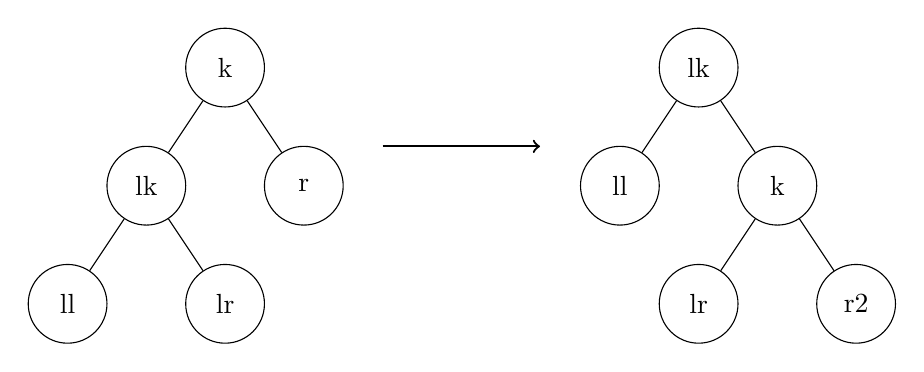
\begin{tikzpicture}[every node/.style={circle, draw, minimum size=1cm}, sibling distance=2cm, level distance=1.5cm]
  % Initial Tree
  \node (k) {k}
    child {
      node (lk) {lk}
      child {node {ll}}
      child {node {lr}}
    }
    child {node {r}};

  % Arrow for Rotation
  \draw[->, thick] (2,-1) -- (4,-1);  % Simple right arrow for rotation

  % After Rotation
  \node[right=5cm of k] (lk2) {lk}
    child {
      node {ll}
    }
    child {
      node (k2) {k}
      child {node {lr}}
      child {node {r2}}
    };
\end{tikzpicture}
\end{center}

\textbf{Left-Right Imbalance (Left-Right Rotation)}
\begin{center}
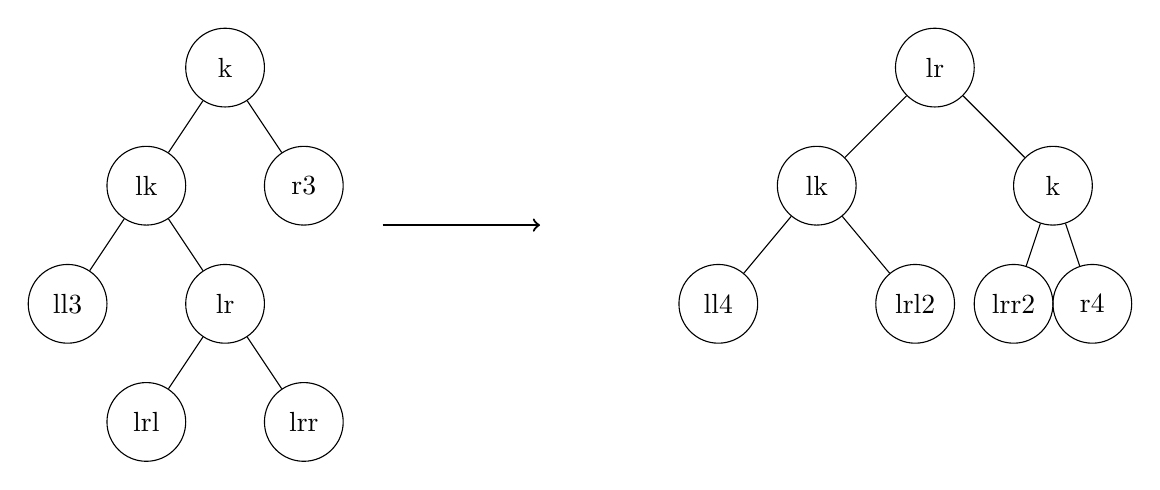
\begin{tikzpicture}[every node/.style={circle, draw, minimum size=1cm}, sibling distance=2 cm, level distance=1.5cm]
  % Initial Tree
  \node (k3) {k}
    child {
      node (lk3) {lk}
      child {node {ll3}}
      child {
        node (lr) {lr}
        child {node {lrl}}
        child {node {lrr}}
      }
    }
    child {node {r3}};

  % Arrow for Rotation
  \draw[->, thick] (2,-2) -- (4,-2);  % Simple left-right arrow for rotation

  % After Rotation
  \node[right=8cm of k3] (lr2) {lr}
    child[sibling distance=3cm] {
      node (lk4) {lk}
      child[sibling distance=2.5cm] {node {ll4}}
      child[sibling distance=2.5cm] {node {lrl2}}
    }
    child[sibling distance=3cm] {
      node (k4) {k}
      child[sibling distance=1cm] {node {lrr2}}
      child[sibling distance=1cm] {node {r4}}
    };
\end{tikzpicture}
\end{center}
  
  This operation works by comparing the heights of the left and right subtrees of the current node. If the left subtree is too tall (i.e., the height difference is greater than one), a rotation is performed. The precise rotation depends on whether the imbalance is caused by the left or right child of the left subtree. The function handles both single and double rotations to restore balance. The balancing of the left subtree is critical for maintaining the AVL property and ensuring that the tree remains balanced after an insertion on the left side.

\begin{defn}{balanceR}

The \texttt{balanceR} function rebalances the tree when the right subtree becomes too tall compared to the left subtree. This can occur after an insertion into the right subtree. If the right subtree becomes imbalanced, \texttt{balanceR} restores balance by performing a rotation. The formal definition in HOL4 is:
\begin{alltt}
	[balanceR_def]
	\HOLthm{def}{AVL_trees.balanceR_def}
\end{alltt}

If the right subtree becomes imbalanced, this function performs the necessary rotation to restore the AVL property and ensure the tree remains balanced.
\end{defn}

\textbf{Right-Right Imbalance (Single Left Rotation)}
\begin{center}
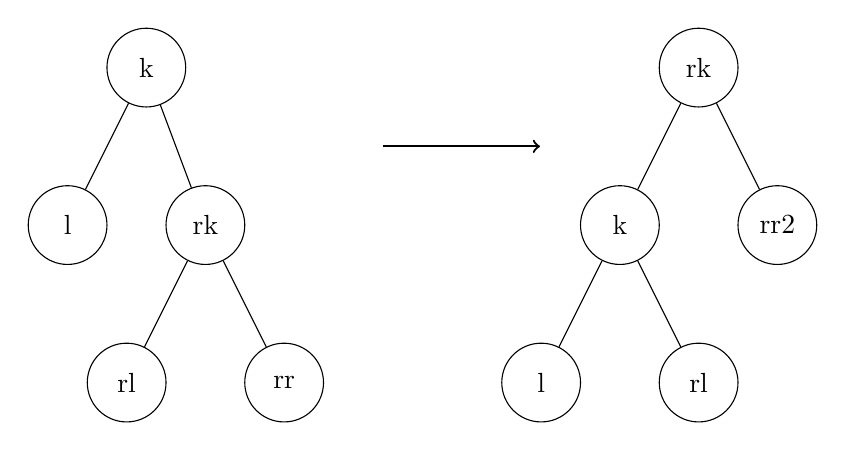
\begin{tikzpicture}[every node/.style={circle, draw, minimum size=1cm}, level distance=2cm]
  % Initial Tree
  \node (k) {k}
    child[sibling distance=2cm] {node {l}}
    child {
      node (rk) {rk}
      child[sibling distance=2cm] {node {rl}}
      child[sibling distance=2cm] {node {rr}}
    };

  % Arrow for Rotation
  \draw[->, thick] (3,-1) -- (5,-1);  % Simple left arrow for rotation

  % After Rotation
  \node[right=6cm of k] (rk2) {rk}
    child[sibling distance=2cm] {
      node (k2) {k}
      child[sibling distance=2cm] {node {l}}
      child[sibling distance=2cm] {node {rl}}
    }
    child[sibling distance=2cm] {node {rr2}};
\end{tikzpicture}
\end{center}

\textbf{Right-Left Imbalance (Right-Left Rotation)}
\begin{center}
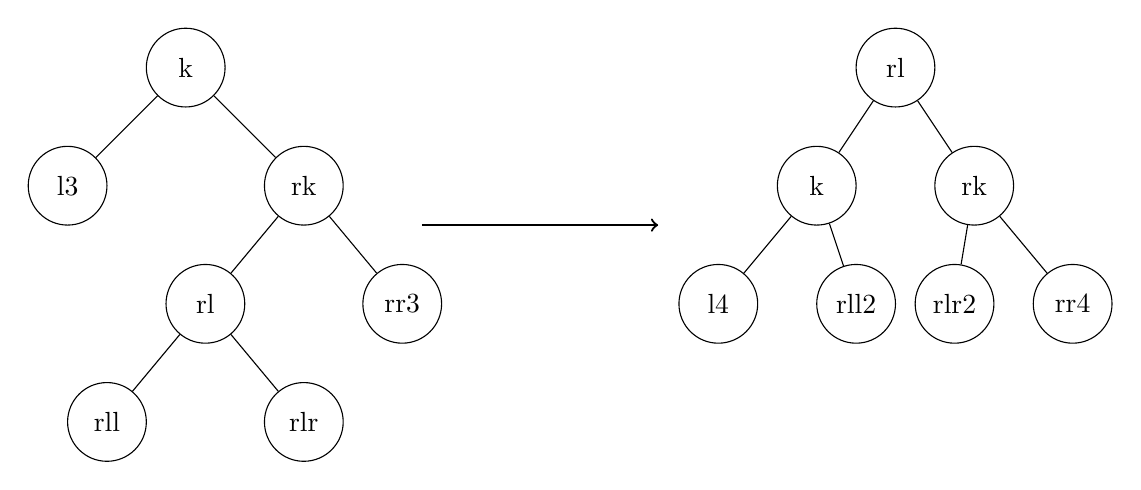
\begin{tikzpicture}[every node/.style={circle, draw, minimum size=1cm}, sibling distance=3cm, level distance=1.5cm]
  % Initial Tree
  \node (k3) {k}
    child[sibling distance=3cm] {node {l3}}
    child {
      node (rk3) {rk}
      child[sibling distance=2.5cm] {
        node (rl) {rl}
        child[sibling distance=2.5cm] {node {rll}}
        child[sibling distance=2.5cm] {node {rlr}}
      }
      child[sibling distance=2.5cm] {node {rr3}}
    };

  % Arrow for Rotation
  \draw[->, thick] (3,-2) -- (6,-2);  % Simple right-left arrow for rotation

  % After Rotation
  \node[right=8cm of k3] (rl2) {rl}
    child[sibling distance=2cm] {
      node (k4) {k}
      child[sibling distance=2.5cm] {node {l4}}
      child[sibling distance=1cm] {node {rll2}}
    }
    child[sibling distance=2cm] {
      node (rk4) {rk}
      child[sibling distance=0.5cm] {node {rlr2}}
      child[sibling distance=2.5cm] {node {rr4}}
    };
\end{tikzpicture}
\end{center}
  The logic for \texttt{balanceR} is analogous to \texttt{balanceL}, but it handles the case where the right subtree is imbalanced. Similar to \texttt{balanceL}, this function performs either a single or double rotation depending on the structure of the right subtree. Rebalancing the right subtree is essential for maintaining the AVL property after an insertion into the right child of the tree.

\begin{defn}{insert\_avl}

The function \texttt{insert\_avl} is responsible for inserting a new key-value pair into an AVL tree while preserving the AVL property. After inserting the new element, the tree may become unbalanced, so rebalancing operations such as \texttt{balanceL} or \texttt{balanceR} are invoked as necessary. The formal definition in HOL4 is:

\begin{alltt}
	[insert_avl_def]
	\HOLthm{def}{AVL_trees.insert_avl_def}
\end{alltt}


This function ensures that, after inserting a new key-value pair, the AVL property is maintained by invoking the appropriate rebalancing functions (\texttt{balanceL} or \texttt{balanceR}) when necessary.
\end{defn}

In the \texttt{insert\_avl} function, the key-value pair \( (x, v) \) is inserted into the correct position in the tree according to the binary search tree property. If \( x \) is smaller than the current key \( k \), the insertion proceeds in the left subtree. If \( x \) is larger than \( k \), the insertion proceeds in the right subtree. After the insertion, the balance of the tree is checked. If the tree becomes imbalanced, either \texttt{balanceL} or \texttt{balanceR} is applied to restore balance.

The key feature of the \texttt{insert\_avl} function is that it ensures the AVL property is maintained at all levels of the tree. By performing rebalancing operations as needed, the function guarantees that the height of the tree remains logarithmic with respect to the number of nodes. This is crucial for ensuring that search, insertion, and deletion operations can be performed efficiently in \( O(\log n) \) time.

The \texttt{balanceL} and \texttt{balanceR} operations are vital for maintaining the AVL property after modifications to the tree. Without these operations, the tree could become unbalanced, leading to poor performance in subsequent operations. The \texttt{insert\_avl} function ensures that new elements can be added to the tree while keeping it balanced. The careful handling of rotations in both the left and right subtrees allows AVL trees to maintain their optimal height and performance.

\tikzstyle{startstop} = [rectangle, rounded corners, minimum width=3cm, minimum height=1cm, text centered, draw=black, fill=red!30]
\tikzstyle{process} = [rectangle, minimum width=3cm, minimum height=1cm, text centered, draw=black, fill=orange!30]
\tikzstyle{decision} = [diamond, minimum width=3.5cm, minimum height=1cm, text centered, aspect=2, draw=black, fill=green!30]
\tikzstyle{arrow} = [thick,->,>=stealth]


\begin{center}
	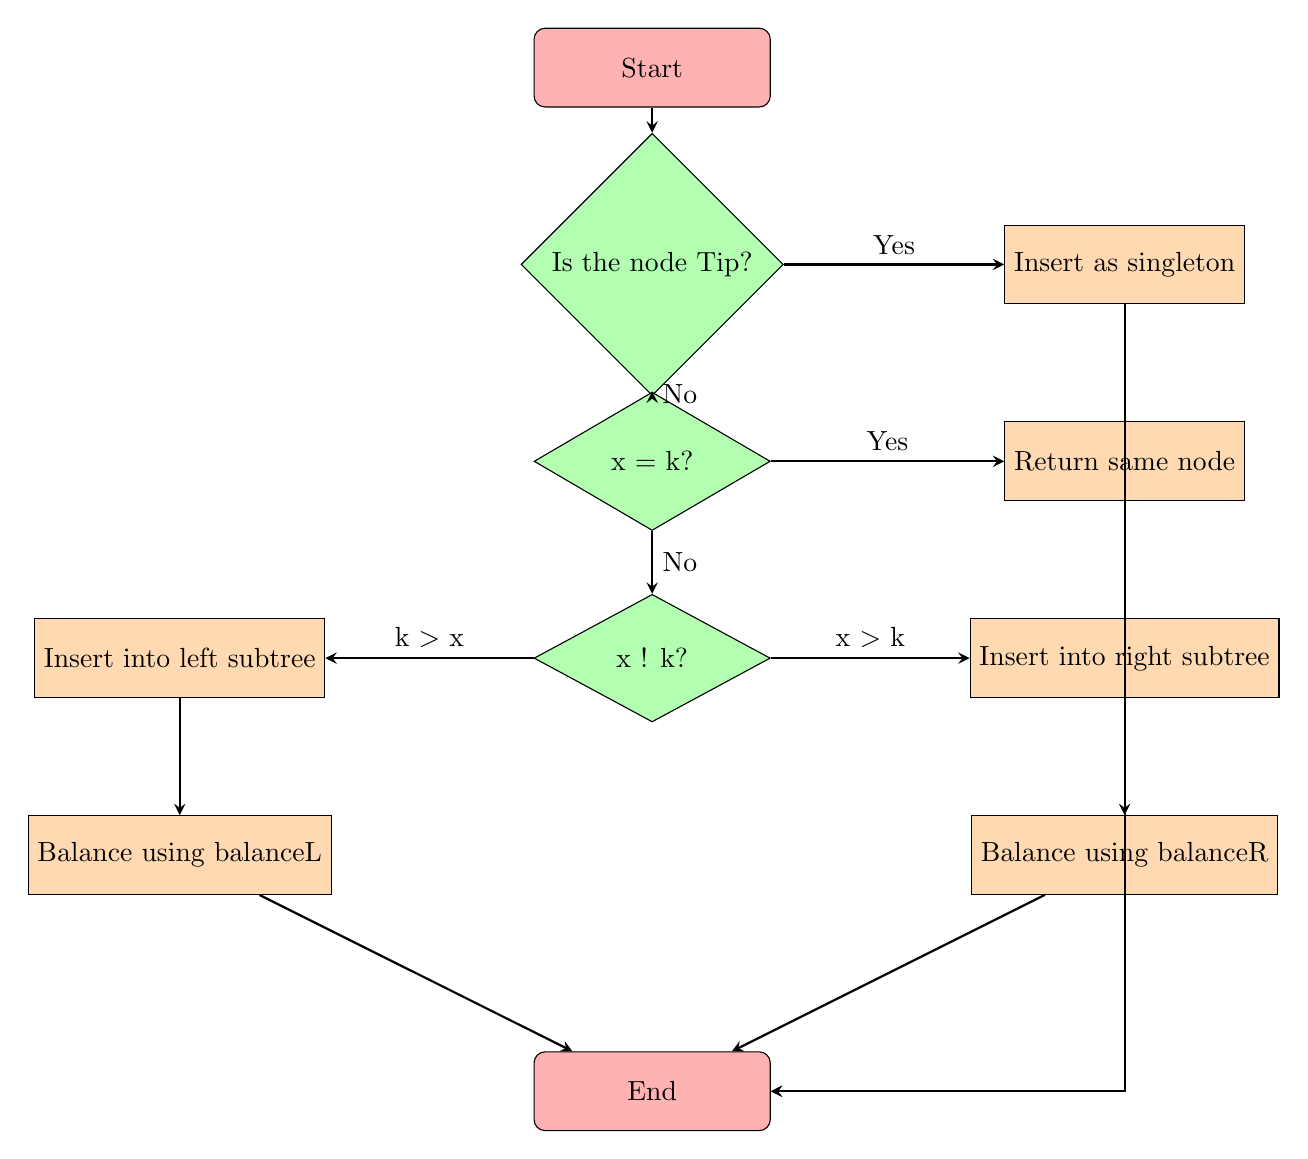
\begin{tikzpicture}[node distance=2.5cm]
		
		% Nodes
		\node (start) [startstop] {Start};
		\node (checktip) [decision, below of=start] {Is the node Tip?};
		\node (singleton) [process, right of=checktip, xshift=3.5cm] {Insert as singleton};
		\node (checkequal) [decision, below of=checktip] {x = k?};
		\node (returnsame) [process, right of=checkequal, xshift=3.5cm] {Return same node};
		\node (checkleft) [decision, below of=checkequal] {x ! k?}; % Fixed less-than symbol
		\node (insertleft) [process, left of=checkleft, xshift=-3.5cm] {Insert into left subtree};
		\node (insertright) [process, right of=checkleft, xshift=3.5cm] {Insert into right subtree};
		\node (balanceL) [process, below of=insertleft] {Balance using balanceL};
		\node (balanceR) [process, below of=insertright] {Balance using balanceR};
		\node (end) [startstop, below of=checkleft, yshift=-3cm] {End};
		
		% Arrows
		\draw [arrow] (start) -- (checktip);
		\draw [arrow] (checktip) -- node[anchor=south] {Yes} (singleton);
		\draw [arrow] (checktip) -- node[anchor=west] {No} (checkequal);
		\draw [arrow] (checkequal) -- node[anchor=south] {Yes} (returnsame);
		\draw [arrow] (checkequal) -- node[anchor=west] {No} (checkleft);
		\draw [arrow] (checkleft) -- node[anchor=south] {k \textgreater\ x} (insertleft); % Fixed greater-than symbol
		\draw [arrow] (checkleft) -- node[anchor=south] {x \textgreater\ k} (insertright); % Fixed greater-than symbol
		\draw [arrow] (insertleft) -- (balanceL);
		\draw [arrow] (insertright) -- (balanceR);
		\draw [arrow] (balanceL) -- (end);
		\draw [arrow] (balanceR) -- (end);
		\draw [arrow] (singleton) |- (end);
		\draw [arrow] (returnsame) |- (end);
		
	\end{tikzpicture}
\end{center}
                   % latex advice
\chapter{Key Theorems for Balancing and Insertion}\label{chap:LaTeXAdvice}

The insertion of elements into an AVL tree must maintain the AVL property, the binary search tree property, and ensure that the keys are updated correctly. The following theorems formally prove the correctness of the insertion algorithm in HOL4. Each theorem plays a critical role in verifying that after an element is inserted, the resulting tree remains balanced, its height is properly adjusted, and the set of keys is correctly updated. These proofs are essential for demonstrating that AVL trees continue to function optimally after an insertion operation.

\begin{thm}{keys\_balanceL}

This theorem states that the set of keys in the tree is preserved when the left balancing operation (\texttt{balanceL}) is performed. The formal statement of the theorem is:


\begin{alltt}
	[keys_balanceL]
	\HOLthm{AVL_trees.keys_balanceL}
\end{alltt}


\end{thm}
This theorem proves that performing the left balancing operation does not alter the set of keys in the AVL tree. After the balancing is applied, the resulting tree still contains the same keys as the original tree, including the root key \( k \), and all the keys from the left subtree \( t1 \) and right subtree \( t2 \).

The proof proceeds by case analysis on the structure of the left subtree. Depending on whether the tree requires a single or double rotation, the set of keys remains unchanged as the nodes are simply rearranged without any keys being added or removed. The correctness of this theorem guarantees that the balancing operation preserves the AVL tree's key set and structure.
\begin{thm}{keys\_balanceR}

This theorem is analogous to the previous one but applies to the right balancing operation (\texttt{balanceR}). The formal statement is:

\begin{alltt}
	[keys_balanceR]
	\HOLthm{AVL_trees.keys_balanceR}
\end{alltt}
\end{thm}

This theorem proves that after performing a right balancing operation, the set of keys in the AVL tree remains unchanged. The key set after balancing still consists of the root key \( k \), along with all the keys from the left subtree \( t1 \) and right subtree \( t2 \).

As with \texttt{keys\_balanceL}, the proof is done by case analysis on the structure of the right subtree. Regardless of the type of rotation (single or double), no keys are removed or added; the nodes are simply rearranged to maintain the tree’s balance. This ensures that the AVL tree remains consistent and its key set is preserved after balancing.

\begin{thm}{keys\_insert}

This theorem proves that after inserting a key \(x\) into an AVL tree \(t\), the resulting set of keys is the union of the set of keys in \(t\) and the singleton set \(\{x\}\). Formally, the theorem is:


\begin{alltt}
	[keys_insert]
	\HOLthm{AVL_trees.keys_insert}
\end{alltt}
\end{thm}

The proof proceeds by structural induction on the AVL tree \( t \), ensuring that the insertion operation correctly places the key \( x \) in either the left or right subtree, depending on its value, while maintaining the binary search tree property. The result confirms that the set of keys is updated correctly after insertion, with no duplicates introduced, thereby preserving the AVL tree's correctness.

\begin{thm}{height\_balL}

This theorem describes the height of an AVL tree after performing a left balancing operation (\texttt{balanceL}). If the left subtree \(l\) has a height that is 2 greater than the right subtree \(r\), then the height of the tree after balancing will be either \(\text{height}(r) + 2\) or \(\text{height}(r) + 3\). Formally:


\begin{alltt}
	[height_balL]
	\HOLthm{AVL_trees.height_balL}
\end{alltt}

\end{thm}

This theorem proves that the height of the tree after left balancing is within a bounded range, ensuring that the AVL tree remains balanced. The proof proceeds by case analysis on the left subtree and shows that balancing adjusts the tree height while maintaining the AVL properties.


\begin{thm}{height\_balR}

This theorem is the symmetric case of \texttt{height\_balL}, describing the height of an AVL tree after performing a right balancing operation (\texttt{balanceR}). If the right subtree \(r\) has a height that is 2 greater than the left subtree \(l\), then the height of the tree after balancing will be either \(\text{height}(l) + 2\) or \(\text{height}(l) + 3\). Formally:


\begin{alltt}
	[height_balR]
	\HOLthm{AVL_trees.height_balR}
\end{alltt}

\end{thm}

This theorem ensures that after right balancing, the tree's height is adjusted within a specific range, maintaining the balanced structure of the AVL tree.


\begin{thm}{height\_balL2}

This theorem deals with the height of an AVL tree after a left balancing operation when the height difference between the left and right subtrees is not 2. It states that in such cases, the height of the resulting tree is simply the maximum height of the left and right subtrees, plus 1:


\begin{alltt}
	[height_balL2]
	\HOLthm{AVL_trees.height_balL2}
\end{alltt}

\end{thm}

This theorem ensures that left balancing adjusts the tree height correctly when there is no significant imbalance between the left and right subtrees.


\begin{thm}{height\_balR2}

This theorem is the symmetric counterpart of \texttt{height\_balL2}, applying to the right balancing operation. It states that when the height difference between the right and left subtrees is not 2, the height of the resulting tree after balancing is the maximum height of the left and right subtrees, plus 1:


\begin{alltt}
	[height_balR2]
	\HOLthm{AVL_trees.height_balR2}
\end{alltt}


\end{thm}

\begin{thm}{avl\_balL}

This theorem proves that performing a left balancing operation on an AVL tree preserves the AVL property, provided that the heights of the left and right subtrees are either equal or differ by 1 or 2:


\begin{alltt}
	[avl_balL]
	\HOLthm{AVL_trees.avl_balL}
\end{alltt}


\end{thm}

\begin{thm}{avl\_balR}

This theorem is the symmetric case of \texttt{avl\_balL}. It proves that performing a right balancing operation preserves the AVL property, provided the heights of the subtrees are either equal or differ by 1 or 2:


\begin{alltt}
	[avl_balR]
	\HOLthm{AVL_trees.avl_balR}
\end{alltt}

\end{thm}

\begin{thm}{avl\_tree\_preserves\_avl}

This theorem guarantees that the AVL property is preserved when constructing a binary tree using the \texttt{tree} function, as long as both left and right subtrees are AVL trees and their heights are either equal or differ by at most 1:


\begin{alltt}
	[avl_tree_preserves_avl]
	\HOLthm{AVL_trees.avl_tree_preserves_avl}
\end{alltt}
\end{thm}

This theorem ensures that the AVL tree property is preserved whenever a tree is constructed from balanced subtrees.

\begin{thm}{avl\_insert\_aux}

This theorem proves that inserting a new key \(k\) and value \(v\) into an AVL tree preserves the AVL property. It also states that the height of the tree will either remain the same or increase by 1:


\begin{alltt}
	[avl_insert_aux]
	\HOLthm{AVL_trees.avl_insert_aux}
\end{alltt}

\end{thm}

This theorem guarantees that the insertion of a new key preserves both the AVL tree’s balance and its height properties.

The proofs of these theorems collectively demonstrate that the insertion operation in AVL trees is both correct and efficient. By ensuring that the AVL property is preserved, the height is properly adjusted, and the set of keys is correctly updated, these theorems guarantee that AVL trees continue to function optimally after insertion. Furthermore, the balancing operations (handled by \texttt{balanceL} and \texttt{balanceR}) ensure that any imbalance introduced by the insertion is corrected, preserving the logarithmic height of the tree and ensuring efficient search and insertion times.                       % notes on marking
\chapter{Deletion in AVL Trees}\label{chap:LaTeXAdvice}

Deleting a node from an AVL tree is a more complex operation than insertion because we not only need to remove the node but also ensure that the tree remains balanced afterward. AVL trees maintain their efficiency by guaranteeing that the height difference between the left and right subtrees of any node is at most one. To preserve this property, deletion operations in AVL trees are often followed by one or more rebalancing steps.

This section introduces two key definitions used in the deletion process: \texttt{remove\_max}, which handles finding and removing the maximum element in a subtree, and \texttt{delete\_avl}, the main function for deleting a node from an AVL tree while maintaining the AVL property.

\begin{defn}{remove\_max}

The \texttt{remove\_max} function is designed to find and remove the maximum element from a given subtree. This operation is particularly important when deleting a node with two children, as we often replace the deleted node with its predecessor—the maximum node from the left subtree. The formal definition of \texttt{remove\_max} is as follows:


\begin{alltt}
	[remove_max]
	\HOLthm[def]{AVL_trees.remove_max_def}
\end{alltt}

\end{defn}


\texttt{remove\_max} works as follows:
\begin{itemize}
    \item If the right subtree of a node is empty (represented by \texttt{Tip}), the node itself is the maximum node, and the left subtree becomes the new subtree after the removal of the maximum node.
    \item If the right subtree is not empty, the function recursively calls itself on the right subtree to find the maximum node, and then it rebalances the resulting tree using the \texttt{balanceL} function. This ensures that the AVL property is preserved after the maximum node is removed.
\end{itemize}

This function is crucial in maintaining the AVL tree structure, particularly when we need to replace a node with its predecessor during deletion.

\begin{defn}{delete\_avl}

The main operation for deleting a node from an AVL tree is defined by the \texttt{delete\_avl} function. This function removes the key \( x \) from the tree while preserving the AVL property by balancing the tree when necessary. The formal definition is:


\begin{alltt}
	[delete_avl_def]
	\HOLthm[def]{AVL_trees.delete_avl_def}
\end{alltt}

This definition ensures that the AVL property is preserved after deleting a node from the tree by applying the appropriate balancing operations (\texttt{balanceL} or \texttt{balanceR}) depending on which subtree the deletion occurs in.
\end{defn}


The \texttt{delete\_avl} function works in the following way:
\begin{itemize}
    \item If the tree is empty (i.e., \texttt{Tip}), there is nothing to delete, and the function simply returns \texttt{Tip}.
    \item If the key \( x \) matches the root key \( k \), then the function must delete this node. There are four cases to handle:
    \begin{itemize}
        \item If both the left and right subtrees are empty (\texttt{Tip}), the result is \texttt{Tip}, indicating that the tree is now empty.
        \item If only the left subtree is empty, the right subtree replaces the current node.
        \item If only the right subtree is empty, the left subtree replaces the current node.
        \item If both subtrees are non-empty, the function finds the maximum node from the left subtree using \texttt{remove\_max}, and replaces the current node with this maximum node. Afterward, the tree is rebalanced using the \texttt{balanceR} function to ensure that the AVL property is maintained.
    \end{itemize}
    \item If the key \( x \) is less than the root key \( k \), the function recursively deletes \( x \) from the left subtree, and then rebalances the resulting tree using \texttt{balanceR}.
    \item If the key \( x \) is greater than the root key \( k \), the function recursively deletes \( x \) from the right subtree, and then rebalances the resulting tree using \texttt{balanceL}.
\end{itemize}

This function ensures that the AVL tree remains balanced after a deletion by applying the appropriate rebalancing operation, either \texttt{balanceL} or \texttt{balanceR}, depending on which subtree was modified.

\subsubsection{Balancing After Deletion}

After a node is deleted from an AVL tree, the tree may become unbalanced. To restore balance, AVL trees use two main types of balancing operations:
\begin{itemize}
    \item \textbf{Left Balancing (\texttt{balanceL})}: This is used when the right subtree becomes taller than the left subtree. Left balancing involves single or double rotations to redistribute the height and restore the AVL property.
    \item \textbf{Right Balancing (\texttt{balanceR})}: This is used when the left subtree becomes taller than the right subtree. Right balancing, similar to left balancing, involves rotations that adjust the tree's height to ensure balance.
\end{itemize}

These balancing operations guarantee that the AVL tree remains balanced after any deletion. Without rebalancing, the tree could degrade into an unbalanced binary search tree, losing the logarithmic height that makes AVL trees efficient for operations such as search, insertion, and deletion.

\subsubsection{Handling the Deletion of Nodes with Two Children}

The most complex case occurs when the node to be deleted has two children. In this situation, AVL trees follow a common strategy in binary search trees: replacing the node with either its predecessor (the maximum node from the left subtree) or its successor (the minimum node from the right subtree). This ensures that the binary search tree property is maintained.

In the \texttt{delete\_avl} function, we use the predecessor (maximum node from the left subtree). Once the predecessor is removed from the left subtree using \texttt{remove\_max}, the tree is rebalanced using \texttt{balanceR} to restore the AVL property.

Deletion in AVL trees involves several steps: finding the node to be deleted, removing it while preserving the structure of the tree, and rebalancing the tree as necessary to ensure that the AVL property is maintained. Whether the node is a leaf, has one child, or has two children, the function carefully handles each case and uses the \texttt{balanceL} and \texttt{balanceR} operations to maintain the balance of the tree.

The result is an AVL tree that remains efficient for all operations, with logarithmic height in the number of nodes, ensuring optimal performance even after deletions.


\begin{center}
	\resizebox{1\textwidth}{!}{
		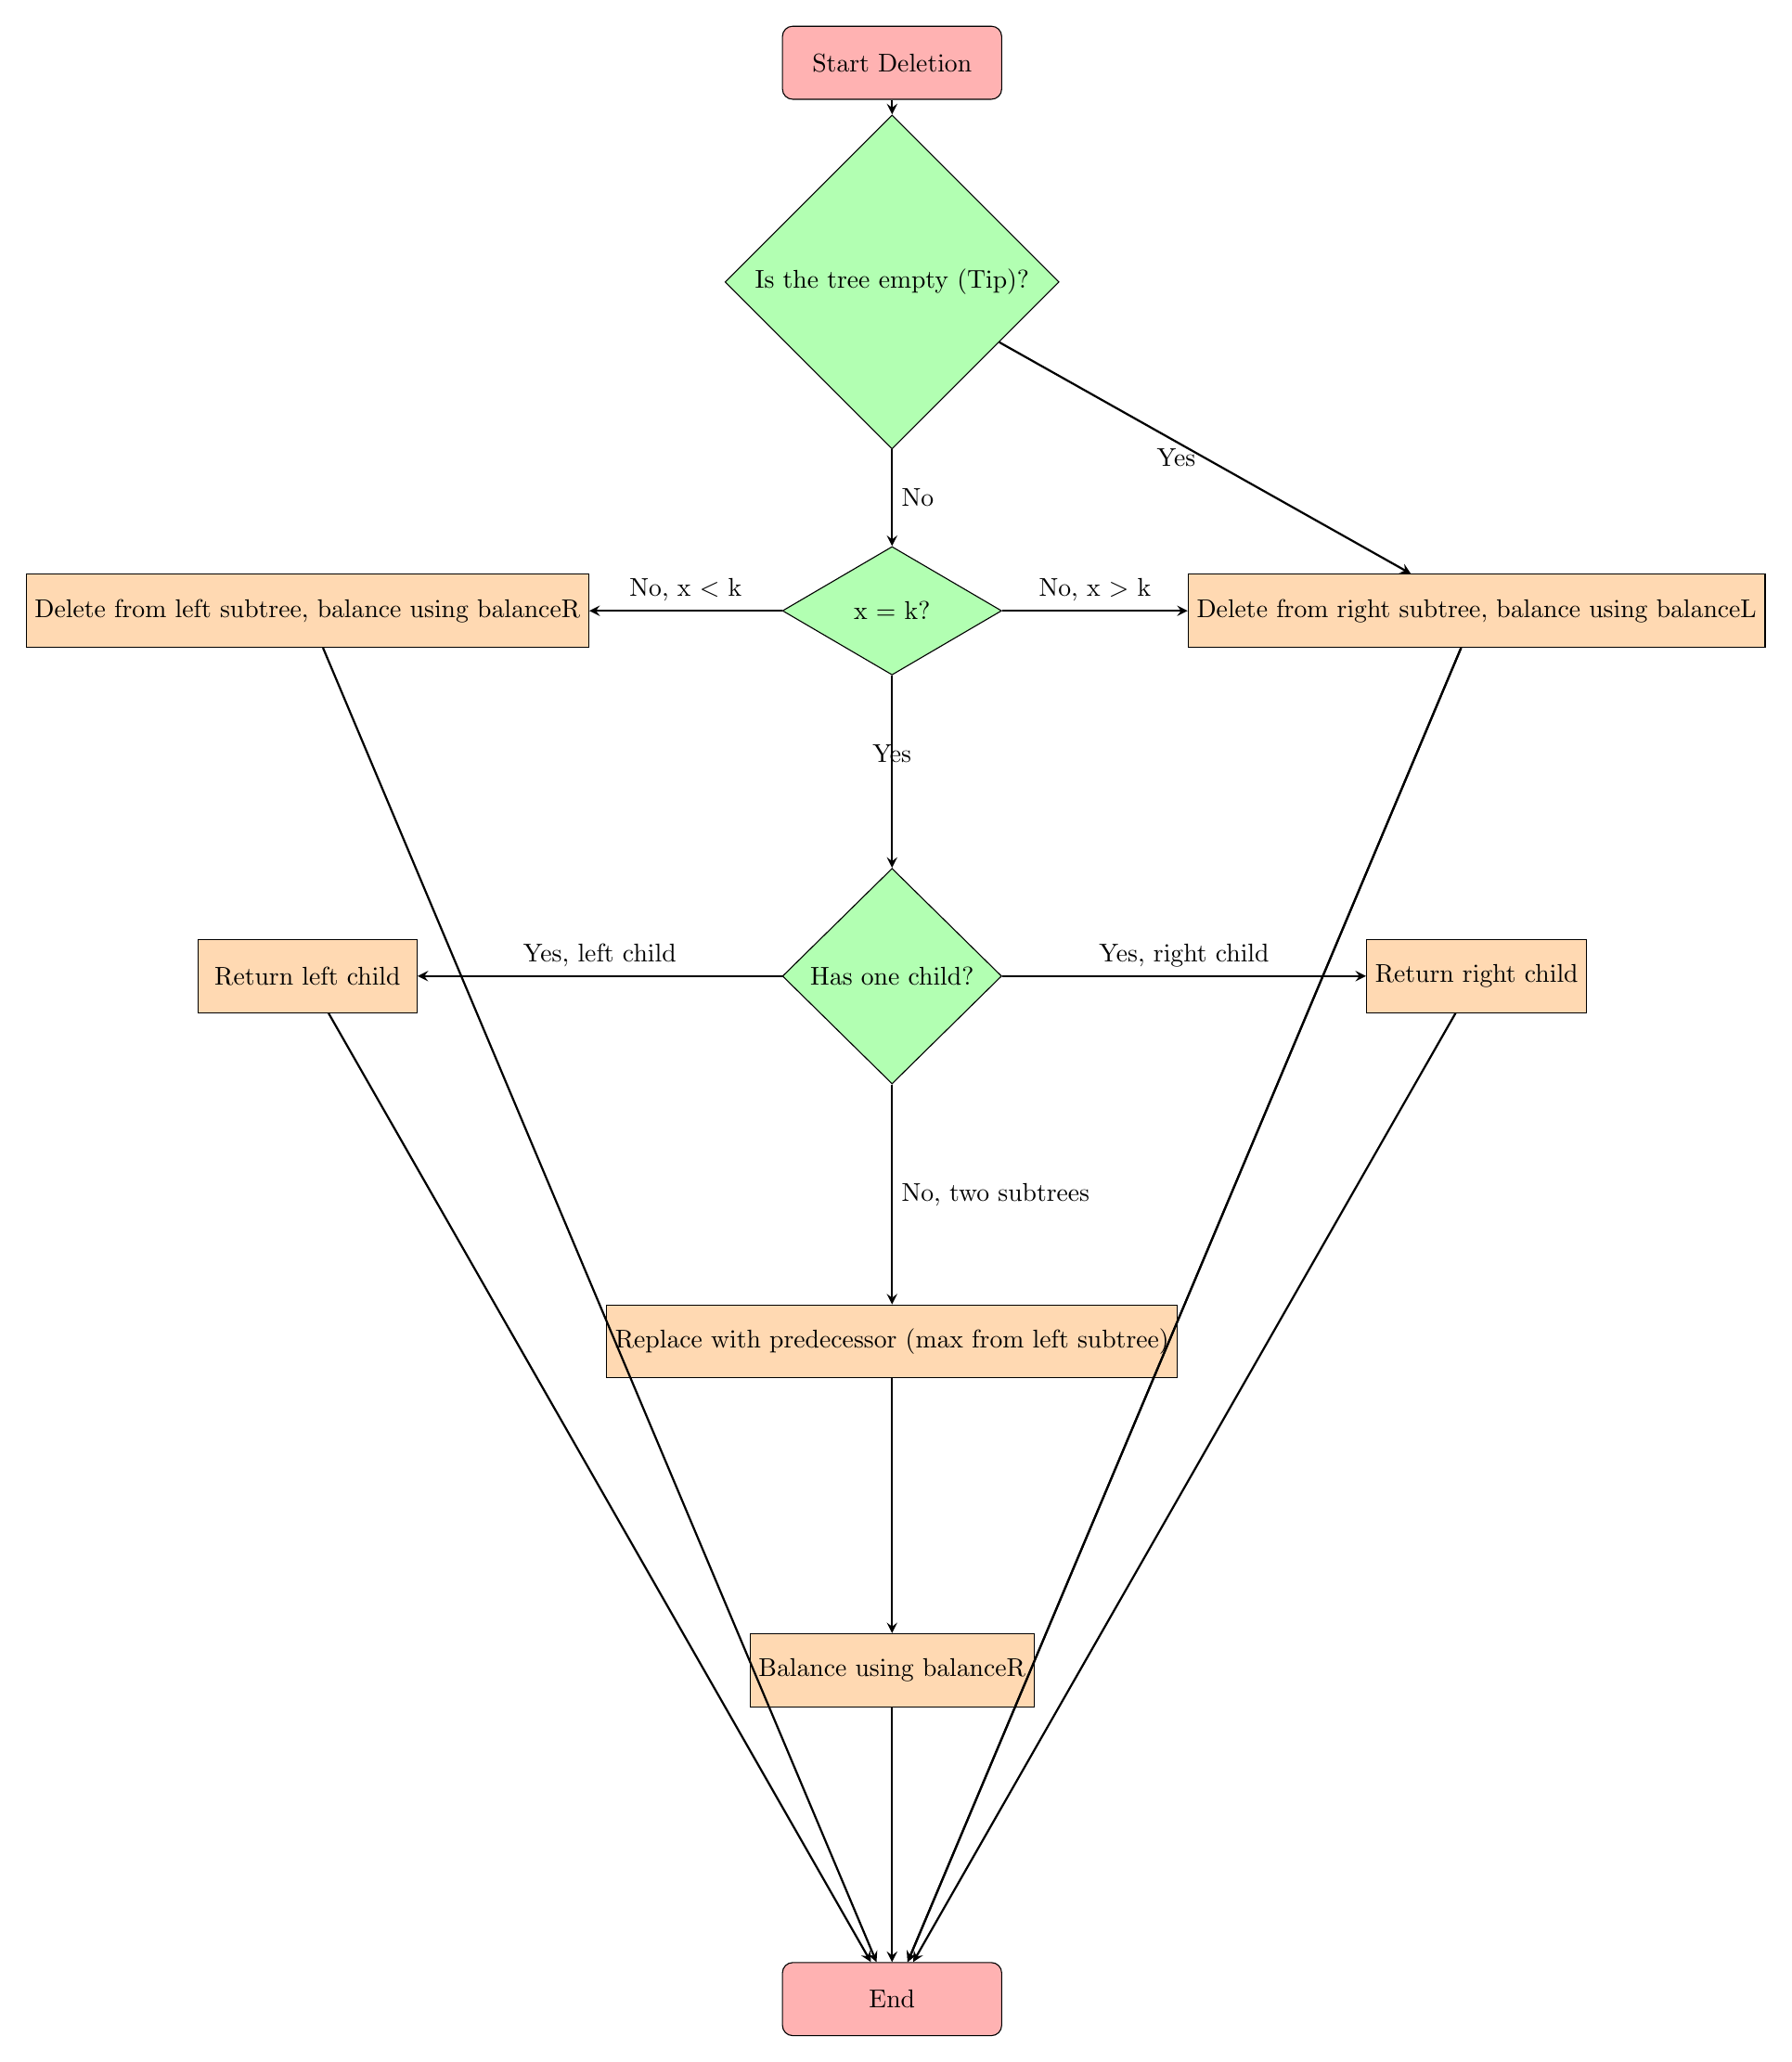
\begin{tikzpicture}[node distance=3cm] % Increased node distance for better spacing
			
			\node (start) [startstop] {Start Deletion};
			\node (checktip) [decision, below of=start] {Is the tree empty (Tip)?};
			\node (checkkey) [decision, below of=checktip, yshift=-1.5cm] {x = k?}; % Increased yshift for more space
			\node (leafcase) [process, right of=checkkey, xshift=5cm] {Delete and return Tip}; % Increased xshift
			\node (onechild) [decision, below of=checkkey, yshift=-2cm] {Has one child?}; % Increased yshift for more space
			\node (replaceleft) [process, left of=onechild, xshift=-5cm] {Return left child}; % Increased xshift
			\node (replaceright) [process, right of=onechild, xshift=5cm] {Return right child}; % Increased xshift
			\node (twosubtrees) [process, below of=onechild, yshift=-2cm] {Replace with predecessor (max from left subtree)};
			\node (removeandbalance) [process, below of=twosubtrees, yshift=-1.5cm] {Balance using balanceR};
			\node (recursionleft) [process, left of=checkkey, xshift=-5cm] {Delete from left subtree, balance using balanceR}; % Increased xshift
			\node (recursionright) [process, right of=checkkey, xshift=5cm] {Delete from right subtree, balance using balanceL}; % Increased xshift
			\node (end) [startstop, below of=removeandbalance, yshift=-1.5cm] {End};
			
			\draw [arrow] (start) -- (checktip);
			\draw [arrow] (checktip) -- node[anchor=east] {Yes} (leafcase);
			\draw [arrow] (checktip) -- node[anchor=west] {No} (checkkey);
			\draw [arrow] (checkkey) -- node[anchor=south] {Yes} (onechild);
			\draw [arrow] (onechild) -- node[anchor=south] {Yes, left child} (replaceleft);
			\draw [arrow] (onechild) -- node[anchor=south] {Yes, right child} (replaceright);
			\draw [arrow] (onechild) -- node[anchor=west] {No, two subtrees} (twosubtrees);
			\draw [arrow] (twosubtrees) -- (removeandbalance);
			\draw [arrow] (checkkey) -- node[anchor=south] {No, x \textless\ k} (recursionleft); % Fixed left arrow label
			\draw [arrow] (checkkey) -- node[anchor=south] {No, x \textgreater\ k} (recursionright); % Fixed right arrow label
			\draw [arrow] (removeandbalance) -- (end);
			\draw [arrow] (leafcase) -- (end);
			\draw [arrow] (replaceleft) -- (end);
			\draw [arrow] (replaceright) -- (end);
			\draw [arrow] (recursionleft) -- (end);
			\draw [arrow] (recursionright) -- (end);
			
		\end{tikzpicture}
	}
\end{center}                    % evaluation
\chapter{Lookup in AVL Trees}\label{chap:LaTeXAdvice}

The lookup operation in an AVL tree is used to find the value associated with a given key. AVL trees, being a form of binary search tree, support efficient lookup operations with a time complexity of \( O(\log n) \), where \( n \) is the number of nodes in the tree. The lookup function follows the structure of a binary search, comparing the target key with the keys in the tree and recursively traversing the left or right subtree until the key is found or a leaf node is reached.

The formal definition of the \texttt{lookup\_avl} function is as follows:

\begin{defn}{lookup\_avl}

The \texttt{lookup\_avl} function searches for a key \( x \) in an AVL tree. It returns the corresponding value if the key is found, otherwise, it returns \texttt{NONE}. The formal definition of \texttt{lookup\_avl} is:


\begin{alltt}
	[lookup_avl_def]
	\HOLthm[def]{AVL_trees.lookup_avl_def}
\end{alltt}

\end{defn}


The lookup operation works as follows:
\begin{itemize}
    \item If the tree is empty (represented by \texttt{Tip}), the function returns \texttt{NONE}, indicating that the key does not exist in the tree.
    \item If the key \( x \) matches the root key \( k \), the function returns \texttt{SOME kv}, where \( kv \) is the value associated with the key \( k \).
    \item If the key \( x \) is less than \( k \), the function recursively searches the left subtree.
    \item If the key \( x \) is greater than \( k \), the function recursively searches the right subtree.
\end{itemize}

\subsubsection{Binary Search Property}

The \texttt{lookup\_avl} function takes advantage of the binary search property of AVL trees. Since the tree is ordered, we can compare the target key \( x \) with the root key \( k \) to determine whether to search the left or right subtree. This reduces the number of nodes that need to be examined, ensuring that the lookup operation has logarithmic time complexity.

If the target key \( x \) is found, the function returns the value associated with the key. Otherwise, if the search reaches an empty subtree (\texttt{Tip}), the function returns \texttt{NONE}, indicating that the key is not present in the tree.

\subsubsection{Efficiency of Lookup in AVL Trees}

One of the key advantages of AVL trees is that they maintain balance, which guarantees that the tree's height remains logarithmic in relation to the number of nodes. This balance ensures that lookup operations are efficient, even in the worst case. Without balancing, a binary search tree could degenerate into a linked list, resulting in linear time complexity for lookups. However, AVL trees avoid this worst-case scenario by enforcing the height balance property.

The \texttt{lookup\_avl} function operates in \( O(\log n) \) time because the height of the tree is always proportional to \( \log n \), where \( n \) is the number of nodes in the tree. This makes AVL trees an excellent choice for applications that require frequent lookups and need to maintain optimal performance.

The lookup operation in AVL trees is a simple, recursive process that leverages the tree's binary search structure to efficiently locate a key. If the key is present, the value associated with it is returned. If the key is not found, the function returns \texttt{NONE}. The balance property of AVL trees ensures that lookup operations are performed in logarithmic time, making AVL trees highly efficient for search operations in both average and worst-case scenarios.
                    % conclusion
\chapter{Design Integration in HOL4}\label{chap:LaTeXAdvice}

The formal verification of data structures in HOL4 requires not only defining the structure and properties of the data structure but also ensuring that it integrates seamlessly with the theorem prover's existing framework. In this section, we focus on the design considerations, adaptations, and extensions made to formalize AVL trees within HOL4, a higher-order logic theorem prover. These adaptations were necessary to ensure that the formalization of AVL trees fits into HOL4’s framework, allowing future developers to build upon this work easily and enabling the reuse of existing libraries within HOL4.

\subsection{Adapting the AVL Formalization to HOL4’s Framework}

The HOL4 theorem prover has a robust framework for formalizing mathematical structures and reasoning about their properties. However, any new formalization must be carefully integrated into this existing ecosystem. In the case of AVL trees, several key design decisions were made to ensure that the formalization fits smoothly into HOL4’s libraries and adheres to its conventions. Below, we discuss the key design adaptations and the rationale behind them.


\subsection{Choosing the Appropriate Datatype Representation}

HOL4 provides a rich environment for defining custom datatypes, which is essential for formalizing data structures like AVL trees. The choice of datatype representation is crucial because it affects how the formalization interacts with existing tools and libraries within HOL4. AVL trees, as a recursive data structure, are defined in HOL4 using the following datatype:

\[
\texttt{avl\_tree} = \texttt{Tip} \, | \, \texttt{Bin} \, \texttt{int} \, \texttt{num} \, 'a \, \texttt{avl\_tree} \, \texttt{avl\_tree}
\]

This representation captures the essential structure of AVL trees:
\begin{itemize}
    \item \texttt{Tip}: Represents an empty tree.
    \item \texttt{Bin}: Represents a node in the tree, containing:
        \begin{itemize}
            \item \textbf{int}: The balance factor, which stores the difference in height between the left and right subtrees.
            \item \textbf{num}: The key associated with the node.
            \item \textbf{'a avl\_tree}: The left subtree.
            \item \textbf{'a avl\_tree}: The right subtree.
        \end{itemize}
\end{itemize}

This datatype was chosen because it allows easy integration with HOL4’s built-in tools for recursive data structures and pattern matching. By using a recursive datatype, we ensure that the formalization is compatible with HOL4's proof automation tools, such as  \( Induct_on \), which are commonly used for reasoning about recursive functions and data structures.

\subsection{Seamless Integration with HOL4’s Existing Libraries}

A key design consideration was ensuring that the AVL tree formalization could reuse existing libraries within HOL4, such as the arithmetic, list, and set theory libraries. Reusing these libraries reduces redundancy, simplifies the formalization process, and enables more robust proof automation.

For example, the existing list and set libraries in HOL4 were leveraged for defining and proving properties about the keys in an AVL tree. The `keys` function, which retrieves the set of keys in an AVL tree, is integrated with HOL4’s existing set theory library:

\begin{alltt}
	[keys_def]
	\HOLthm[def]{AVL_trees.keys_def}
\end{alltt}


This integration allows us to make use of HOL4’s extensive set-theoretic reasoning capabilities, enabling efficient proofs about the contents of the tree, such as proving that a key exists in the tree after an insertion \(keys_insert\) or that the set of keys is updated correctly after an operation.

By designing the formalization to interface with HOL4’s existing libraries, we ensure that future work can build upon this foundation without needing to reimplement basic functionality. This modularity and reusability are key strengths of the HOL4 framework, and they were critical design considerations during the development of the AVL tree formalization.

\subsection{Handling Recursive Functions and Theorem}

Recursive functions are essential for formalizing AVL tree operations, such as height calculation, insertion, and balancing. In HOL4, recursive functions must be carefully defined to ensure that they terminate and are well-formed. The formalization of AVL trees makes extensive use of recursion to define operations like \(insert_avl\), \(balanceL\), and \(balanceR\).

For example, the function \(insert_avl\) is defined recursively to ensure that it can insert a new element into an AVL tree while preserving the AVL property. This function must handle both the base case (inserting into an empty tree) and the recursive case (inserting into a non-empty tree). To integrate this recursive function with HOL4’s framework, termination must be guaranteed:

\begin{alltt}
	[insert_avl_def]
	\HOLthm{AVL_trees.insert_avl_def}
\end{alltt}

In this recursive definition, the height of the tree decreases with each recursive call, which ensures that the recursion terminates. HOL4’s support for reasoning about recursive functions allows us to prove that \(insert avl\) correctly maintains the AVL property and terminates for all inputs. This recursive approach is also extended to other operations, such as \(balanceL\) and \(balanceR\), which are used to restore the AVL property after an insertion.

\subsection{Designing Efficient Proof Strategies}

To verify the correctness of the AVL tree formalization, a series of theorems must be proven about the properties of AVL trees, such as their height, balance, and the set of keys. HOL4 provides various proof strategies, such as induction, case analysis, and automated tactics, to facilitate the proof process.

One of the key challenges in designing the formalization was choosing efficient proof strategies that could handle the complexity of recursive functions and the AVL property. For example, proving that the height of the tree is logarithmic with respect to the number of nodes requires an inductive proof that leverages the recursive structure of the AVL tree and its relationship with the Fibonacci sequence.

Another challenge was proving that the \(balanceL\) and \(balanceR\) functions correctly restore the AVL property after an insertion. These proofs require reasoning about the height of the subtrees and ensuring that the balance factor remains within the allowed range. The use of HOL4’s automated proof tactics, such as \(REWRITE TAC\) and \(INDUCT TAC\), allowed these proofs to be constructed efficiently.

\subsection{Exporting the Formalization}

Once the formalization was completed, it was exported as part of HOL4’s growing library of verified data structures. The export process ensures that the formalization can be easily reused and extended by other developers working within the HOL4 framework. By integrating the AVL tree formalization into HOL4’s existing libraries, we ensure that future work can build upon this foundation, whether for educational purposes, research, or practical applications involving verified data structures.

In summary, the formalization of AVL trees in HOL4 required several key design adaptations to fit seamlessly into HOL4’s existing framework. These adaptations included choosing a suitable recursive datatype representation, integrating with existing HOL4 libraries, designing recursive functions with termination in mind, and employing efficient proof strategies to verify the correctness of AVL tree operations. By making these design choices, we ensure that the AVL tree formalization is both robust and reusable, providing a solid foundation for future work in HOL4. 
\chapter{Comparision with existing theories}\label{chap:LaTeXAdvice}

\subsection{Isabelle’s AVL Tree Implementation}

Isabelle/HOL provides a formalization of AVL trees that is widely regarded as one of the most complete and influential formalizations in the field of theorem proving. Isabelle's formalization of AVL trees follows a monolithic approach, where all the components—data type definitions, auxiliary functions, and theorems—are tightly integrated into one comprehensive theory. This contrasts with the more modular structure that HOL4 typically encourages, where components are often distributed across different theories for reusability and composability.

\subsubsection{Datatype Representation in Isabelle}
In Isabelle, the AVL tree is defined as a recursive data structure using a datatype declaration. Here is the definition from Isabelle’s formalization:

\[
\text{datatype} \, (\text{set\_of}: \, 'a) \, \text{tree} = 
\text{ET} \, | \, \text{MKT} \, 'a \, (\text{'a \, tree}) \, (\text{'a \, tree}) \, \text{nat}
\]

This datatype closely mirrors the one used in HOL4 but includes an additional `nat` parameter in each node, which explicitly stores the height of the tree as part of the node’s structure. This explicit height parameter differs from the HOL4 approach, where the height of a tree is computed recursively rather than being stored within the tree structure. While storing the height as part of the node structure simplifies some operations, such as balancing and checking AVL properties, it increases the complexity of maintaining the correct height values during tree mutations (insertions and deletions).

In HOL4, by contrast, the height is computed dynamically using a recursive function. The AVL tree in HOL4 is defined as follows:

\[
\text{avl\_tree} = \text{Tip} \, | \, \text{Bin} \, (\text{int}) \, (\text{num}) \, ('a) \, (\text{avl\_tree}) \, (\text{avl\_tree})
\]

This definition uses a balance factor (an integer representing the height difference between the left and right subtrees) instead of explicitly storing the height as in Isabelle. This design decision aligns with the traditional AVL tree structure and maintains the dynamic computation of tree properties rather than encoding them directly in the data structure.

\subsubsection{Height Calculation}
The height of an AVL tree in Isabelle is calculated using a primitive recursive function:

\[
\text{height} \, (\text{ET}) = 0
\]
\[
\text{height} \, (\text{MKT} \, x \, l \, r \, h) = \max(\text{height}(l), \text{height}(r)) + 1
\]
In HOL4, a similar function calculates the height of the tree, but it uses a recursive definition rather than reading the height from the tree’s structure. The HOL4 height function is:

\[
\text{height}(\text{Tip}) = 0
\]
\[
\text{height}(\text{Bin} \, h \, k \, v \, l \, r) = \max(\text{height}(l), \text{height}(r)) + 1
\]

While both functions ultimately compute the height of the tree, Isabelle’s approach benefits from faster height lookups, as the height is stored in each node. However, this comes at the cost of maintaining this value during tree mutations, increasing the complexity of operations like insertion and deletion.

\subsubsection{AVL Tree Property (avl Predicate)}
Both Isabelle and HOL4 define a predicate to ensure that a tree satisfies the AVL property. In Isabelle, the AVL property is enforced as follows:

\begin{align*}
	\text{avl}(\text{MKT} \, x \, l \, r \, h) = & \left( (\text{height}(l) = \text{height}(r) \right. \\
	& \lor \, \text{height}(l) = \text{height}(r) + 1 \\
	& \lor \, \text{height}(r) = \text{height}(l) + 1) \\
	& \land \, h = \max(\text{height}(l), \text{height}(r)) + 1 \\
	& \land \, \text{avl}(l) \, \land \, \text{avl}(r) \left. \right)
\end{align*}


This function checks that the tree is balanced by ensuring the heights of the left and right subtrees differ by at most one, and it also verifies that the stored height value is consistent with the actual height of the tree.

In HOL4, the AVL property is similarly enforced, but using the balance factor instead of explicitly stored heights:

\[
\text{avl}(\text{Tip}) = \text{T}
\]
\begin{align*}
	\text{avl}(\text{Bin} \, bf \, k \, v \, l \, r) = & \left( (\text{height}(l) = \text{height}(r) \right. \\
	& \lor \, \text{height}(l) = \text{height}(r) + 1 \\
	& \lor \, \text{height}(r) = \text{height}(l) + 1) \\
	& \land \, bf = \text{\&height}(r) - \text{\&height}(l) \\
	& \land \, \text{avl}(l) \, \land \, \text{avl}(r) \left. \right)
\end{align*}

Both implementations ensure that the AVL property is maintained, but the HOL4 version dynamically calculates the height difference between subtrees using the balance factor, while the Isabelle version relies on pre-computed height values.

\subsubsection{Insertion and Balancing}

The insertion operation in Isabelle is more complex due to the explicit height field in each node. Here’s the definition for inserting a new element into the tree:

\[
\text{insert}(x, \text{ET}) = \text{MKT}(x, \text{ET}, \text{ET}, 1)
\]
\begin{align*}
	\text{insert}(x, \text{MKT}(n, l, r, h)) = & 
	\begin{cases}
		x = n \Rightarrow \text{MKT}(n, l, r, h), \\
		x < n \Rightarrow \text{mkt\_bal\_l}(n, \text{insert}(x, l), r), \\
		x > n \Rightarrow \text{mkt\_bal\_r}(n, l, \text{insert}(x, r))
	\end{cases}
\end{align*}

This function balances the tree after an insertion using two auxiliary functions, \(mkt_bal_l\) and \(mkt_bal_r\), which handle left and right rotations, respectively. These balancing functions are more complex in Isabelle because they need to maintain the height field after rebalancing.

In HOL4, the insertion function does not need to maintain an explicit height field. Instead, it focuses on maintaining the balance factor, which simplifies the balancing operations:

\[
\text{insert\_avl}(x, v, \text{Tip}) = \text{singleton\_avl}(x, v)
\]
\begin{align*}
	\text{insert\_avl}(x, v, \text{Bin}(bf, k, kv, l, r)) = 
	& \begin{cases}
		x = k \Rightarrow \text{Bin}(bf, k, kv, l, r), \\
		x < k \Rightarrow \text{balanceL}(k, kv, \text{insert\_avl}(x, v, l), r), \\
		x > k \Rightarrow \text{balanceR}(k, kv, l, \text{insert\_avl}(x, v, r))
	\end{cases}
\end{align*}

Here, `balanceL` and `balanceR` handle left and right rotations, ensuring the AVL property is restored after insertion. Since the height is calculated recursively, there is no need to explicitly update it during these operations.

\subsubsection{Efficiency and Trade-offs}

The primary trade-off between the two implementations lies in the efficiency of height lookups and the complexity of maintaining balance. Isabelle's approach, which stores the height in each node, allows for faster lookups during insertion and deletion but increases the complexity of maintaining correct height values. In contrast, HOL4’s implementation dynamically calculates the height and uses a balance factor, simplifying the maintenance of tree invariants but potentially making height lookups slightly slower.

Overall, the HOL4 implementation is more in line with the traditional AVL tree design, focusing on balance factors, while Isabelle’s version opts for an explicit height field, which influences both performance and complexity.

\subsubsection{Proof Techniques and Automation}
Isabelle’s AVL tree formalization leverages Isabelle’s powerful proof automation tools, such as `simp` and `auto`, to simplify the proof of correctness for insertion and deletion operations. For example, the following lemma ensures that the AVL property is maintained after insertion:

\begin{thm}{avl\_insert\_aux}
	
	This theorem proves that inserting a key into an AVL tree preserves the AVL property and that the height of the tree is either unchanged or increased by one. The formal statement is:
	
	\[
	\text{assumes:} \, \text{avl}(t)
	\]
	\[
	\text{shows:} \, \text{avl}(\text{insert}(x, t)) \quad \land
	\]
	\[
	\left( \text{height}(\text{insert}(x, t)) = \text{height}(t) \, \lor \, 
	\text{height}(\text{insert}(x, t)) = \text{height}(t) + 1 \right)
	\]
	
	This theorem guarantees that after inserting a new key \( x \) into an AVL tree \( t \), the AVL property is preserved, and the height of the tree will either remain the same or increase by one.
	
\end{thm}
HOL4 employs similar proof strategies but relies more heavily on explicit recursion and case analysis to establish the same properties. The modularity of HOL4’s proof tactics, such as \(rw\) (rewrite) and \(induct_on\), allows for fine-grained control over the proof process.

\subsubsection{Summary of Differences}
In summary, Isabelle’s AVL tree formalization takes a more explicit approach by storing the height of each tree node, which simplifies height lookups but complicates insertion and deletion operations. HOL4’s formalization, on the other hand, maintains the traditional AVL tree structure by dynamically calculating heights and using a balance factor to ensure the tree remains balanced. Both approaches have their advantages and trade-offs, with Isabelle’s approach favoring efficient height lookups and HOL4’s approach favoring simplicity in tree mutations.

\subsection{Balanced\_bst in HOL4}

In contrast to Isabelle’s formalization of AVL trees, HOL4 \cite{HOLBalancedBST} provides a modular and flexible formalization of balanced binary search trees (BSTs), known as \texttt{balanced\_bst}. HOL4's approach is characterized by its focus on modularity, where different components such as balance operations, key comparison, and height management are separated into reusable theories. This modular design encourages compositional reasoning and reusability of core components across different theories.

\subsubsection{Data Type Representation in HOL4}
In HOL4, the \texttt{balanced\_bst} type follows the typical structure of binary search trees, with nodes that store keys, values, and left and right subtrees. This differs from Isabelle's AVL tree formalization, which includes an explicit height parameter stored in each node. HOL4 avoids encoding height directly into the datatype, opting instead for recursive functions to manage balancing operations and height computations.

The HOL4 definition for \texttt{balanced\_bst} is as follows:

\[
\text{balanced\_bst} = \text{Tip} \, | \, \text{Bin} \, (\text{size}) \, (\text{key}) \, (\text{value}) \, (\text{balanced\_bst}) \, (\text{balanced\_bst})
\]

In this definition, the tree is either empty (\texttt{Tip}) or a binary node (\texttt{Bin}) that stores the size of the subtree, a key, a value, and references to left and right subtrees. Unlike Isabelle, which stores an explicit height value, HOL4 calculates properties such as height recursively as needed.

\subsubsection{Balancing and Height Calculation}
HOL4’s balancing functions dynamically compute the balance factor using the height difference between subtrees. This contrasts with Isabelle’s approach, where the height is stored within each node.

The height of a tree in HOL4 is computed as follows:

\[
\text{height}(\text{Tip}) = 0
\]
\[
\text{height}(\text{Bin} \, \_ \, \_ \, \_ \, l \, r) = \max(\text{height}(l), \text{height}(r)) + 1
\]

In this recursive definition, the height of an empty tree (\texttt{Tip}) is zero, while the height of a node is the maximum height of its subtrees plus one. This approach mirrors the classic AVL tree structure, maintaining balance based on dynamic height calculations rather than pre-stored height values.

\subsubsection{Balancing Operations}
The balancing operations in HOL4 focus on restoring the AVL property by applying left and right rotations when needed. The \texttt{balance\_L} and \texttt{balance\_R} functions are used to rebalance the tree after an insertion or deletion.

\[
\text{balanceL}(k, v, l, r) = 
\begin{cases}
	\text{if} \, \text{height}(l) > \text{height}(r) + 1, \, \text{then} \, \text{rotateR}(k, v, l, r), \\
	\text{else} \, \text{Bin}(\_, k, v, l, r)
\end{cases}
\]

\[
\text{balanceR}(k, v, l, r) = 
\begin{cases}
	\text{if} \, \text{height}(r) > \text{height}(l) + 1, \, \text{then} \, \text{rotateL}(k, v, l, r), \\
	\text{else} \, \text{Bin}(\_, k, v, l, r)
\end{cases}
\]


These functions ensure that the balance factor remains within acceptable limits by rotating the tree when the height difference between left and right subtrees exceeds 1. Unlike Isabelle, which recalculates and stores the height explicitly in each node, HOL4’s balancing is based solely on recursive height calculations.

\subsubsection{Trade-offs and Design Considerations}
The primary difference between HOL4’s and Isabelle’s implementations lies in the handling of height. While Isabelle stores the height explicitly within each node, HOL4 opts for recursive height calculations. This decision simplifies the node structure in HOL4 but may lead to slightly slower height lookups compared to Isabelle’s approach.

Moreover, HOL4's modular design promotes code reuse and flexibility, allowing developers to extend or adapt the core balanced tree structure without tightly coupling all components into a single monolithic theory. In contrast, Isabelle's formalization integrates all components into a single theory, which can be beneficial for comprehensive reasoning but may limit modularity.

\subsubsection{Proof Techniques and Automation}
The proof strategies employed in HOL4 leverage its modularity and tactics such as \texttt{rw} (rewrite) and \texttt{induct\_on} for case analysis and recursion. HOL4 requires more explicit handling of recursion and case distinctions compared to Isabelle, where powerful automation tools like \texttt{simp} and \texttt{auto} play a central role in proofs. The modularity of HOL4’s proof system allows for precise control over individual components of the proof, making it a preferred choice for fine-grained formal reasoning.

\subsubsection{Summary of Differences}
In summary, HOL4’s \texttt{balanced\_bst} formalization maintains the traditional AVL tree structure by dynamically calculating heights and focusing on balance factors. This contrasts with Isabelle’s more explicit approach, where the height is stored within each node, allowing for faster height lookups but requiring more complex maintenance of tree properties. HOL4’s design favors modularity, flexibility, and dynamic height computation, whereas Isabelle’s approach favors efficiency in height lookups and monolithic integration.

%\cite{IsabelleAVL} 
\chapter{Future Work}\label{chap:LaTeXAdvice}
While significant progress has been made in formalizing AVL trees, there are still several open problems and extensions that deserve further exploration. In this section, we outline some of the key areas that can be addressed in future work, with a particular focus on the relationship between Fibonacci sequences and AVL tree properties, as well as the formal proof of tree depth and node count relations.

\subsection*{Fibonacci Sequence to logarithmic nature}

The Fibonacci sequence \( 0, 1, 1, 2, 3, 5, 8, 13, 21, \dots \) is defined by the following recurrence relation:

\[
F(0) = 0, \quad F(1) = 1, \quad F(i) = F(i - 1) + F(i - 2) \quad \text{for } i \geq 2
\]

This sequence has been studied for centuries, and it exhibits fascinating mathematical properties. The elements of the Fibonacci sequence can be expressed as linear combinations with fixed coefficients of the powers of the roots of the polynomial \( x^2 - x - 1 \), whose roots are given by:

\[
\phi = \frac{1 + \sqrt{5}}{2} \approx 1.618 \quad \text{and} \quad \hat{\phi} = \frac{1 - \sqrt{5}}{2} \approx -0.618
\]

Here, \( \phi \) is known as the golden ratio. The Fibonacci sequence is then approximated as follows:

\[
F(i) = \frac{1}{\sqrt{5}} \left( \phi^i - \hat{\phi}^i \right) \quad \text{for } i \geq 0
\]

Since the absolute value of \( \hat{\phi} \) is smaller than 1, the term \( \hat{\phi}^i \) quickly becomes negligible as \( i \) increases, allowing for a good approximation of \( F(i) \) using just the first term:

\[
F(i) \approx \frac{1}{\sqrt{5}} \phi^i
\]

This approximation is especially relevant for studying AVL trees, as the number of nodes \( n \) in an AVL tree of depth \( k \) is bounded by a relationship involving Fibonacci numbers. Specifically, the number of nodes satisfies:

\[
n \geq N(k) = F(k + 3) - 1 \approx \frac{1}{\sqrt{5}} \phi^{k+3} - 1
\]

This relationship provides an exponential bound on the number of nodes in terms of the tree’s depth, which is crucial for understanding the efficiency and scalability of AVL trees.

\subsection*{Current Achievements and Future Directions}

In this work, we have successfully proved the relationship between the Fibonacci sequence and the node count of AVL trees. Specifically, we demonstrated that the minimum number of nodes \( N(k) \) in an AVL tree of depth \( k \) is related to Fibonacci numbers. This result is important as it shows that the structure of AVL trees is nearly optimal in terms of space efficiency, with the height growing logarithmically with the number of nodes.

However, proving deeper relations between Fibonacci numbers and AVL trees remains an open problem. For example, while we have established the relation between node count and Fibonacci numbers, we have yet to fully prove the relationship between Fibonacci numbers and tree depth. According to **Theorem 5.1**, the number of nodes \( n \) in an AVL tree of depth \( k \) is at least exponential in \( k \), meaning \( n \geq a^k \) for some constant \( a > 1 \). This exponential bound still needs to be formalized rigorously within the context of the Fibonacci sequence.

The bounds on the depth \( k \) of AVL trees are also connected to the logarithmic nature of Fibonacci numbers. Specifically, we know that:

\[
\log_\phi \left( \sqrt{5}(n + 1) \right) \geq k + 3
\]

This provides a bound on the depth of AVL trees, even in the worst-case scenario, where the depth is at most 44\% larger than in the best-case scenario. Additionally, the average depth can be shown to be approximately \( 1.04 \log_2 n \), indicating that AVL trees offer highly efficient access and search operations.

Future work will focus on rigorously proving these bounds, using Fibonacci-based recurrence relations to formalize the relationships between node count and depth in AVL trees. Specifically, proving the relationship expressed in Theorem 5.1 in its full generality remains an open challenge, as it requires careful analysis of the recursive nature of AVL trees and their relationship to Fibonacci numbers.


\subsection*{Proving Properties of Deletion and Lookup for Trees}

While this work has formalized many aspects of AVL trees, including insertion, balancing, and the relationship between node count and Fibonacci numbers, proving properties related to deletion and lookup operations remains an open problem for future research.

\textbf{Deletion}: The deletion operation in AVL trees is more complex than insertion, as it involves removing a node while ensuring that the tree remains balanced. Although we have defined the \texttt{delete\_avl} function and explored its behavior in various cases (e.g., nodes with zero, one, or two children), a formal proof of its correctness, specifically regarding maintaining the AVL property, has yet to be completed. Proving that the tree remains balanced after every deletion operation, and that the height of the tree either remains the same or decreases by one, is critical for ensuring the efficiency of the deletion process.

\textbf{Lookup}: Similarly, the lookup operation, defined by the \texttt{lookup\_avl} function, has not been formally verified. The lookup function searches for a key in the tree by recursively traversing the left or right subtree based on the comparison with the root key. While the function’s behavior appears correct, a formal proof that the operation maintains the binary search tree property and that the time complexity is \( O(\log n) \) in the worst case is still required.

Both deletion and lookup operations are fundamental to the practical use of AVL trees, and formal verification of these operations will ensure that AVL trees remain efficient for all operations. Future work will focus on developing formal proofs for these operations, demonstrating that they preserve the key properties of AVL trees, such as balance and logarithmic height.

By completing the proofs for deletion and lookup, we can provide a fully verified framework for AVL trees, ensuring that all tree operations are both correct and efficient.

 
\chapter{Conclusion}\label{chap:LaTeXAdvice}

This thesis presents a comprehensive formalization of AVL trees within the HOL4 theorem prover, contributing to the broader effort of enriching HOL4's library of verified data structures. The formalization covers key aspects of AVL trees, including recursive data structures, balance conditions, height constraints, and the associated balancing operations. Through this work, we have formalized the core properties that ensure AVL trees maintain their logarithmic height and efficiency for search, insertion, and deletion operations.

A central achievement of this thesis is the detailed specification and proof of AVL tree correctness, particularly focusing on the invariant that ensures the height difference between subtrees remains bounded. By formalizing the recursive relationships between nodes, this work reinforces the importance of AVL trees in guaranteeing optimal performance for balanced binary search trees.

In comparing the HOL4 formalization with other theorem proving environments such as Isabelle/HOL, we identified significant differences in the design decisions that impact efficiency, maintainability, and complexity. While Isabelle opts for an explicit height parameter stored within each node, HOL4 dynamically computes the height during recursive operations. This leads to a trade-off between the simplicity of the AVL tree structure and the performance of height lookups during rebalancing operations. The comparative analysis highlights both the strengths and limitations of each approach, providing insights into different formalization strategies.

This formalization is not only an academic exercise but also a practical contribution to the ongoing development of verified data structures in HOL4. The methods and techniques developed here can be extended to other self-balancing tree structures or more complex data structures, further enriching the HOL4 ecosystem. Future work can build on this foundation, integrating AVL trees into more advanced applications such as formalized compilers, automated reasoning tools, or verified databases.

In conclusion, this thesis advances the state of the art in formal verification by providing a rigorous, reusable, and modular formalization of AVL trees in HOL4. It serves as a stepping stone for future developments, encouraging further exploration and refinement of formally verified data structures within theorem proving systems. 



% literature
\bibliographystyle{anuthesis} % or plainnat or whatever
\cleardoublepage\phantomsection
% see https://tex.stackexchange.com/questions/60556/link-to-bibliography-in-the-toc-fails
\bibliography{bib}


%% APPENDIX
\section*{Appendix: AVL\_trees Theory}

\newcommand{\HOLAVLXXtreesDate}{23 Ottobre 2024}
\newcommand{\HOLAVLXXtreesTime}{11:01}
\begin{SaveVerbatim}{HOLAVLXXtreesDatatypesavlXXtree}
\HOLFreeVar{avl\HOLTokenUnderscore{}tree} = \HOLConst{Tip} \HOLTokenBar{} \HOLConst{Bin} \HOLTyOp{int} \HOLTyOp{num} \alpha{} (\alpha{} \HOLTyOp{avl_tree}) (\alpha{} \HOLTyOp{avl_tree})
\end{SaveVerbatim}
\newcommand{\HOLAVLXXtreesDatatypesavlXXtree}{\UseVerbatim{HOLAVLXXtreesDatatypesavlXXtree}}
\newcommand{\HOLAVLXXtreesDatatypes}{
\HOLAVLXXtreesDatatypesavlXXtree}
\begin{SaveVerbatim}{HOLAVLXXtreesDefinitionsavlXXdef}
\HOLTokenTurnstile{} (\HOLConst{avl} \HOLConst{Tip} \HOLSymConst{\HOLTokenEquiv{}} \HOLConst{T}) \HOLSymConst{\HOLTokenConj{}}
   \HOLSymConst{\HOLTokenForall{}}\HOLBoundVar{bf} \HOLBoundVar{k} \HOLBoundVar{v} \HOLBoundVar{l} \HOLBoundVar{r}.
     \HOLConst{avl} (\HOLConst{Bin} \HOLBoundVar{bf} \HOLBoundVar{k} \HOLBoundVar{v} \HOLBoundVar{l} \HOLBoundVar{r}) \HOLSymConst{\HOLTokenEquiv{}}
     (\HOLConst{height} \HOLBoundVar{l} \HOLSymConst{=} \HOLConst{height} \HOLBoundVar{r} \HOLSymConst{\HOLTokenDisj{}} \HOLConst{height} \HOLBoundVar{l} \HOLSymConst{=} \HOLConst{height} \HOLBoundVar{r} \HOLSymConst{\ensuremath{+}} \HOLNumLit{1} \HOLSymConst{\HOLTokenDisj{}}
      \HOLConst{height} \HOLBoundVar{r} \HOLSymConst{=} \HOLConst{height} \HOLBoundVar{l} \HOLSymConst{\ensuremath{+}} \HOLNumLit{1}) \HOLSymConst{\HOLTokenConj{}} \HOLBoundVar{bf} \HOLSymConst{=} \HOLSymConst{\&}\HOLConst{height} \HOLBoundVar{r} \HOLSymConst{\ensuremath{-}} \HOLSymConst{\&}\HOLConst{height} \HOLBoundVar{l} \HOLSymConst{\HOLTokenConj{}}
     \HOLConst{avl} \HOLBoundVar{l} \HOLSymConst{\HOLTokenConj{}} \HOLConst{avl} \HOLBoundVar{r}
\end{SaveVerbatim}
\newcommand{\HOLAVLXXtreesDefinitionsavlXXdef}{\UseVerbatim{HOLAVLXXtreesDefinitionsavlXXdef}}
\begin{SaveVerbatim}{HOLAVLXXtreesDefinitionsbalanceLXXdef}
\HOLTokenTurnstile{} \HOLSymConst{\HOLTokenForall{}}\HOLBoundVar{k} \HOLBoundVar{v} \HOLBoundVar{l} \HOLBoundVar{r}.
     \HOLConst{balanceL} \HOLBoundVar{k} \HOLBoundVar{v} \HOLBoundVar{l} \HOLBoundVar{r} \HOLSymConst{=}
     \HOLKeyword{if} \HOLConst{height} \HOLBoundVar{l} \HOLSymConst{=} \HOLConst{height} \HOLBoundVar{r} \HOLSymConst{\ensuremath{+}} \HOLNumLit{2} \HOLKeyword{then}
       \HOLKeyword{case} \HOLBoundVar{l} \HOLKeyword{of}
         \HOLConst{Tip} \HOLTokenImp{} \HOLConst{tree} \HOLBoundVar{k} \HOLBoundVar{v} \HOLBoundVar{l} \HOLBoundVar{r}
       \HOLTokenBar{} \HOLConst{Bin} \ensuremath{\HOLBoundVar{v}\sb{\mathrm{1}}} \HOLBoundVar{lk} \HOLBoundVar{lv} \HOLBoundVar{ll} \HOLBoundVar{lr} \HOLTokenImp{}
         \HOLKeyword{if} \HOLConst{height} \HOLBoundVar{ll} \HOLSymConst{\HOLTokenLt{}} \HOLConst{height} \HOLBoundVar{lr} \HOLKeyword{then}
           \HOLKeyword{case} \HOLBoundVar{lr} \HOLKeyword{of}
             \HOLConst{Tip} \HOLTokenImp{} \HOLConst{tree} \HOLBoundVar{lk} \HOLBoundVar{lv} \HOLBoundVar{ll} (\HOLConst{tree} \HOLBoundVar{k} \HOLBoundVar{v} \HOLBoundVar{lr} \HOLBoundVar{r})
           \HOLTokenBar{} \HOLConst{Bin} \ensuremath{\HOLBoundVar{v}\sb{\mathrm{6}}} \HOLBoundVar{lrn} \HOLBoundVar{lrv} \HOLBoundVar{lrl} \HOLBoundVar{lrr} \HOLTokenImp{}
             \HOLConst{tree} \HOLBoundVar{lrn} \HOLBoundVar{lrv} (\HOLConst{tree} \HOLBoundVar{lk} \HOLBoundVar{lv} \HOLBoundVar{ll} \HOLBoundVar{lrl}) (\HOLConst{tree} \HOLBoundVar{k} \HOLBoundVar{v} \HOLBoundVar{lrr} \HOLBoundVar{r})
         \HOLKeyword{else} \HOLConst{tree} \HOLBoundVar{lk} \HOLBoundVar{lv} \HOLBoundVar{ll} (\HOLConst{tree} \HOLBoundVar{k} \HOLBoundVar{v} \HOLBoundVar{lr} \HOLBoundVar{r})
     \HOLKeyword{else} \HOLConst{tree} \HOLBoundVar{k} \HOLBoundVar{v} \HOLBoundVar{l} \HOLBoundVar{r}
\end{SaveVerbatim}
\newcommand{\HOLAVLXXtreesDefinitionsbalanceLXXdef}{\UseVerbatim{HOLAVLXXtreesDefinitionsbalanceLXXdef}}
\begin{SaveVerbatim}{HOLAVLXXtreesDefinitionsbalanceRXXdef}
\HOLTokenTurnstile{} \HOLSymConst{\HOLTokenForall{}}\HOLBoundVar{k} \HOLBoundVar{v} \HOLBoundVar{l} \HOLBoundVar{r}.
     \HOLConst{balanceR} \HOLBoundVar{k} \HOLBoundVar{v} \HOLBoundVar{l} \HOLBoundVar{r} \HOLSymConst{=}
     \HOLKeyword{if} \HOLConst{height} \HOLBoundVar{r} \HOLSymConst{=} \HOLConst{height} \HOLBoundVar{l} \HOLSymConst{\ensuremath{+}} \HOLNumLit{2} \HOLKeyword{then}
       \HOLKeyword{case} \HOLBoundVar{r} \HOLKeyword{of}
         \HOLConst{Tip} \HOLTokenImp{} \HOLConst{tree} \HOLBoundVar{k} \HOLBoundVar{v} \HOLBoundVar{l} \HOLBoundVar{r}
       \HOLTokenBar{} \HOLConst{Bin} \ensuremath{\HOLBoundVar{v}\sb{\mathrm{1}}} \HOLBoundVar{rk} \HOLBoundVar{rv} \HOLBoundVar{rl} \HOLBoundVar{rr} \HOLTokenImp{}
         \HOLKeyword{if} \HOLConst{height} \HOLBoundVar{rl} \HOLSymConst{\HOLTokenGt{}} \HOLConst{height} \HOLBoundVar{rr} \HOLKeyword{then}
           \HOLKeyword{case} \HOLBoundVar{rl} \HOLKeyword{of}
             \HOLConst{Tip} \HOLTokenImp{} \HOLConst{tree} \HOLBoundVar{rk} \HOLBoundVar{rv} (\HOLConst{tree} \HOLBoundVar{k} \HOLBoundVar{v} \HOLBoundVar{l} \HOLBoundVar{rl}) \HOLBoundVar{rr}
           \HOLTokenBar{} \HOLConst{Bin} \ensuremath{\HOLBoundVar{v}\sb{\mathrm{6}}} \HOLBoundVar{rln} \HOLBoundVar{rlv} \HOLBoundVar{rll} \HOLBoundVar{rlr} \HOLTokenImp{}
             \HOLConst{tree} \HOLBoundVar{rln} \HOLBoundVar{rlv} (\HOLConst{tree} \HOLBoundVar{k} \HOLBoundVar{v} \HOLBoundVar{l} \HOLBoundVar{rll}) (\HOLConst{tree} \HOLBoundVar{rk} \HOLBoundVar{rv} \HOLBoundVar{rlr} \HOLBoundVar{rr})
         \HOLKeyword{else} \HOLConst{tree} \HOLBoundVar{rk} \HOLBoundVar{rv} (\HOLConst{tree} \HOLBoundVar{k} \HOLBoundVar{v} \HOLBoundVar{l} \HOLBoundVar{rl}) \HOLBoundVar{rr}
     \HOLKeyword{else} \HOLConst{tree} \HOLBoundVar{k} \HOLBoundVar{v} \HOLBoundVar{l} \HOLBoundVar{r}
\end{SaveVerbatim}
\newcommand{\HOLAVLXXtreesDefinitionsbalanceRXXdef}{\UseVerbatim{HOLAVLXXtreesDefinitionsbalanceRXXdef}}
\begin{SaveVerbatim}{HOLAVLXXtreesDefinitionscompleteXXavlXXdef}
\HOLTokenTurnstile{} \HOLConst{complete_avl} \HOLNumLit{0} \HOLSymConst{=} \HOLConst{Tip} \HOLSymConst{\HOLTokenConj{}}
   \HOLSymConst{\HOLTokenForall{}}\HOLBoundVar{n}. \HOLConst{complete_avl} (\HOLConst{SUC} \HOLBoundVar{n}) \HOLSymConst{=}
       \HOLConst{Bin} \HOLNumLit{0} \HOLNumLit{0} \HOLConst{ARB} (\HOLConst{complete_avl} \HOLBoundVar{n}) (\HOLConst{complete_avl} \HOLBoundVar{n})
\end{SaveVerbatim}
\newcommand{\HOLAVLXXtreesDefinitionscompleteXXavlXXdef}{\UseVerbatim{HOLAVLXXtreesDefinitionscompleteXXavlXXdef}}
\begin{SaveVerbatim}{HOLAVLXXtreesDefinitionsdeleteXXavlXXdef}
\HOLTokenTurnstile{} (\HOLSymConst{\HOLTokenForall{}}\HOLBoundVar{x}. \HOLConst{delete_avl} \HOLBoundVar{x} \HOLConst{Tip} \HOLSymConst{=} \HOLConst{Tip}) \HOLSymConst{\HOLTokenConj{}}
   \HOLSymConst{\HOLTokenForall{}}\HOLBoundVar{x} \HOLBoundVar{bf} \HOLBoundVar{k} \HOLBoundVar{kv} \HOLBoundVar{l} \HOLBoundVar{r}.
     \HOLConst{delete_avl} \HOLBoundVar{x} (\HOLConst{Bin} \HOLBoundVar{bf} \HOLBoundVar{k} \HOLBoundVar{kv} \HOLBoundVar{l} \HOLBoundVar{r}) \HOLSymConst{=}
     \HOLKeyword{if} \HOLBoundVar{x} \HOLSymConst{=} \HOLBoundVar{k} \HOLKeyword{then}
       \HOLKeyword{case} (\HOLBoundVar{l}\HOLSymConst{,}\HOLBoundVar{r}) \HOLKeyword{of}
         (\HOLConst{Tip}\HOLSymConst{,}\HOLConst{Tip}) \HOLTokenImp{} \HOLConst{Tip}
       \HOLTokenBar{} (\HOLConst{Tip}\HOLSymConst{,}\HOLConst{Bin} \ensuremath{\HOLBoundVar{v}\sb{\mathrm{27}}} \ensuremath{\HOLBoundVar{v}\sb{\mathrm{28}}} \ensuremath{\HOLBoundVar{v}\sb{\mathrm{29}}} \ensuremath{\HOLBoundVar{v}\sb{\mathrm{30}}} \ensuremath{\HOLBoundVar{v}\sb{\mathrm{31}}}) \HOLTokenImp{} \HOLBoundVar{r}
       \HOLTokenBar{} (\HOLConst{Bin} \ensuremath{\HOLBoundVar{v}\sb{\mathrm{12}}} \ensuremath{\HOLBoundVar{v}\sb{\mathrm{13}}} \ensuremath{\HOLBoundVar{v}\sb{\mathrm{14}}} \ensuremath{\HOLBoundVar{v}\sb{\mathrm{15}}} \ensuremath{\HOLBoundVar{v}\sb{\mathrm{16}}}\HOLSymConst{,}\HOLConst{Tip}) \HOLTokenImp{} \HOLBoundVar{l}
       \HOLTokenBar{} (\HOLConst{Bin} \ensuremath{\HOLBoundVar{v}\sb{\mathrm{12}}} \ensuremath{\HOLBoundVar{v}\sb{\mathrm{13}}} \ensuremath{\HOLBoundVar{v}\sb{\mathrm{14}}} \ensuremath{\HOLBoundVar{v}\sb{\mathrm{15}}} \ensuremath{\HOLBoundVar{v}\sb{\mathrm{16}}}\HOLSymConst{,}\HOLConst{Bin} \ensuremath{\HOLBoundVar{v}\sb{\mathrm{37}}} \ensuremath{\HOLBoundVar{v}\sb{\mathrm{38}}} \ensuremath{\HOLBoundVar{v}\sb{\mathrm{39}}} \ensuremath{\HOLBoundVar{v}\sb{\mathrm{40}}} \ensuremath{\HOLBoundVar{v}\sb{\mathrm{41}}}) \HOLTokenImp{}
         (\HOLKeyword{let}
            (\HOLBoundVar{pred\HOLTokenUnderscore{}k}\HOLSymConst{,}\HOLBoundVar{pred\HOLTokenUnderscore{}v}\HOLSymConst{,}\ensuremath{\HOLBoundVar{l}\sp{\prime{}}}) = \HOLConst{remove_max} \HOLBoundVar{l}
          \HOLKeyword{in}
            \HOLConst{balanceR} \HOLBoundVar{pred\HOLTokenUnderscore{}k} \HOLBoundVar{pred\HOLTokenUnderscore{}v} \ensuremath{\HOLBoundVar{l}\sp{\prime{}}} \HOLBoundVar{r})
     \HOLKeyword{else} \HOLKeyword{if} \HOLBoundVar{x} \HOLSymConst{\HOLTokenLt{}} \HOLBoundVar{k} \HOLKeyword{then} \HOLConst{balanceR} \HOLBoundVar{k} \HOLBoundVar{kv} (\HOLConst{delete_avl} \HOLBoundVar{x} \HOLBoundVar{l}) \HOLBoundVar{r}
     \HOLKeyword{else} \HOLConst{balanceL} \HOLBoundVar{k} \HOLBoundVar{kv} \HOLBoundVar{l} (\HOLConst{delete_avl} \HOLBoundVar{x} \HOLBoundVar{r})
\end{SaveVerbatim}
\newcommand{\HOLAVLXXtreesDefinitionsdeleteXXavlXXdef}{\UseVerbatim{HOLAVLXXtreesDefinitionsdeleteXXavlXXdef}}
\begin{SaveVerbatim}{HOLAVLXXtreesDefinitionsheightXXdef}
\HOLTokenTurnstile{} \HOLConst{height} \HOLConst{Tip} \HOLSymConst{=} \HOLNumLit{0} \HOLSymConst{\HOLTokenConj{}}
   \HOLSymConst{\HOLTokenForall{}}\HOLBoundVar{h} \HOLBoundVar{k} \HOLBoundVar{v} \HOLBoundVar{l} \HOLBoundVar{r}.
     \HOLConst{height} (\HOLConst{Bin} \HOLBoundVar{h} \HOLBoundVar{k} \HOLBoundVar{v} \HOLBoundVar{l} \HOLBoundVar{r}) \HOLSymConst{=} \HOLConst{MAX} (\HOLConst{height} \HOLBoundVar{l}) (\HOLConst{height} \HOLBoundVar{r}) \HOLSymConst{\ensuremath{+}} \HOLNumLit{1}
\end{SaveVerbatim}
\newcommand{\HOLAVLXXtreesDefinitionsheightXXdef}{\UseVerbatim{HOLAVLXXtreesDefinitionsheightXXdef}}
\begin{SaveVerbatim}{HOLAVLXXtreesDefinitionsinsertXXavlXXdef}
\HOLTokenTurnstile{} (\HOLSymConst{\HOLTokenForall{}}\HOLBoundVar{x} \HOLBoundVar{v}. \HOLConst{insert_avl} \HOLBoundVar{x} \HOLBoundVar{v} \HOLConst{Tip} \HOLSymConst{=} \HOLConst{singleton_avl} \HOLBoundVar{x} \HOLBoundVar{v}) \HOLSymConst{\HOLTokenConj{}}
   \HOLSymConst{\HOLTokenForall{}}\HOLBoundVar{x} \HOLBoundVar{v} \HOLBoundVar{bf} \HOLBoundVar{k} \HOLBoundVar{kv} \HOLBoundVar{l} \HOLBoundVar{r}.
     \HOLConst{insert_avl} \HOLBoundVar{x} \HOLBoundVar{v} (\HOLConst{Bin} \HOLBoundVar{bf} \HOLBoundVar{k} \HOLBoundVar{kv} \HOLBoundVar{l} \HOLBoundVar{r}) \HOLSymConst{=}
     \HOLKeyword{if} \HOLBoundVar{x} \HOLSymConst{=} \HOLBoundVar{k} \HOLKeyword{then} \HOLConst{Bin} \HOLBoundVar{bf} \HOLBoundVar{k} \HOLBoundVar{kv} \HOLBoundVar{l} \HOLBoundVar{r}
     \HOLKeyword{else} \HOLKeyword{if} \HOLBoundVar{x} \HOLSymConst{\HOLTokenLt{}} \HOLBoundVar{k} \HOLKeyword{then} \HOLConst{balanceL} \HOLBoundVar{k} \HOLBoundVar{kv} (\HOLConst{insert_avl} \HOLBoundVar{x} \HOLBoundVar{v} \HOLBoundVar{l}) \HOLBoundVar{r}
     \HOLKeyword{else} \HOLConst{balanceR} \HOLBoundVar{k} \HOLBoundVar{kv} \HOLBoundVar{l} (\HOLConst{insert_avl} \HOLBoundVar{x} \HOLBoundVar{v} \HOLBoundVar{r})
\end{SaveVerbatim}
\newcommand{\HOLAVLXXtreesDefinitionsinsertXXavlXXdef}{\UseVerbatim{HOLAVLXXtreesDefinitionsinsertXXavlXXdef}}
\begin{SaveVerbatim}{HOLAVLXXtreesDefinitionskeysXXdef}
\HOLTokenTurnstile{} \HOLConst{keys} \HOLConst{Tip} \HOLSymConst{=} \HOLTokenLeftbrace{}\HOLTokenRightbrace{} \HOLSymConst{\HOLTokenConj{}}
   \HOLSymConst{\HOLTokenForall{}}\ensuremath{\HOLBoundVar{v}\sb{\mathrm{0}}} \HOLBoundVar{k} \HOLBoundVar{v} \HOLBoundVar{l} \HOLBoundVar{r}. \HOLConst{keys} (\HOLConst{Bin} \ensuremath{\HOLBoundVar{v}\sb{\mathrm{0}}} \HOLBoundVar{k} \HOLBoundVar{v} \HOLBoundVar{l} \HOLBoundVar{r}) \HOLSymConst{=} \HOLTokenLeftbrace{}\HOLBoundVar{k}\HOLTokenRightbrace{} \HOLConst{\HOLTokenUnion{}} \HOLConst{keys} \HOLBoundVar{l} \HOLConst{\HOLTokenUnion{}} \HOLConst{keys} \HOLBoundVar{r}
\end{SaveVerbatim}
\newcommand{\HOLAVLXXtreesDefinitionskeysXXdef}{\UseVerbatim{HOLAVLXXtreesDefinitionskeysXXdef}}
\begin{SaveVerbatim}{HOLAVLXXtreesDefinitionslookupXXavlXXdef}
\HOLTokenTurnstile{} (\HOLSymConst{\HOLTokenForall{}}\HOLBoundVar{x}. \HOLConst{lookup_avl} \HOLBoundVar{x} \HOLConst{Tip} \HOLSymConst{=} \HOLConst{NONE}) \HOLSymConst{\HOLTokenConj{}}
   \HOLSymConst{\HOLTokenForall{}}\HOLBoundVar{x} \ensuremath{\HOLBoundVar{v}\sb{\mathrm{0}}} \HOLBoundVar{k} \HOLBoundVar{kv} \HOLBoundVar{l} \HOLBoundVar{r}.
     \HOLConst{lookup_avl} \HOLBoundVar{x} (\HOLConst{Bin} \ensuremath{\HOLBoundVar{v}\sb{\mathrm{0}}} \HOLBoundVar{k} \HOLBoundVar{kv} \HOLBoundVar{l} \HOLBoundVar{r}) \HOLSymConst{=}
     \HOLKeyword{if} \HOLBoundVar{x} \HOLSymConst{=} \HOLBoundVar{k} \HOLKeyword{then} \HOLConst{SOME} \HOLBoundVar{kv}
     \HOLKeyword{else} \HOLKeyword{if} \HOLBoundVar{x} \HOLSymConst{\HOLTokenLt{}} \HOLBoundVar{k} \HOLKeyword{then} \HOLConst{lookup_avl} \HOLBoundVar{x} \HOLBoundVar{l}
     \HOLKeyword{else} \HOLConst{lookup_avl} \HOLBoundVar{x} \HOLBoundVar{r}
\end{SaveVerbatim}
\newcommand{\HOLAVLXXtreesDefinitionslookupXXavlXXdef}{\UseVerbatim{HOLAVLXXtreesDefinitionslookupXXavlXXdef}}
\begin{SaveVerbatim}{HOLAVLXXtreesDefinitionsminimalXXavlXXdef}
\HOLTokenTurnstile{} \HOLSymConst{\HOLTokenForall{}}\HOLBoundVar{t}. \HOLConst{minimal_avl} \HOLBoundVar{t} \HOLSymConst{\HOLTokenEquiv{}}
       \HOLConst{avl} \HOLBoundVar{t} \HOLSymConst{\HOLTokenConj{}}
       \HOLSymConst{\HOLTokenForall{}}\ensuremath{\HOLBoundVar{t}\sp{\prime{}}}.
         \HOLConst{avl} \ensuremath{\HOLBoundVar{t}\sp{\prime{}}} \HOLSymConst{\HOLTokenConj{}} \HOLConst{height} \ensuremath{\HOLBoundVar{t}\sp{\prime{}}} \HOLSymConst{=} \HOLConst{height} \HOLBoundVar{t} \HOLSymConst{\HOLTokenImp{}}
         \HOLConst{node_count} \HOLBoundVar{t} \HOLSymConst{\HOLTokenLeq{}} \HOLConst{node_count} \ensuremath{\HOLBoundVar{t}\sp{\prime{}}}
\end{SaveVerbatim}
\newcommand{\HOLAVLXXtreesDefinitionsminimalXXavlXXdef}{\UseVerbatim{HOLAVLXXtreesDefinitionsminimalXXavlXXdef}}
\begin{SaveVerbatim}{HOLAVLXXtreesDefinitionsNXXdef}
\HOLTokenTurnstile{} \HOLSymConst{\HOLTokenForall{}}\HOLBoundVar{k}. \HOLConst{N} \HOLBoundVar{k} \HOLSymConst{=}
       \HOLConst{MIN_SET} (\HOLConst{IMAGE} \HOLConst{node_count} \HOLTokenLeftbrace{}\HOLBoundVar{x} \HOLTokenBar{} \HOLConst{height} \HOLBoundVar{x} \HOLSymConst{=} \HOLBoundVar{k} \HOLSymConst{\HOLTokenConj{}} \HOLConst{avl} \HOLBoundVar{x}\HOLTokenRightbrace{})
\end{SaveVerbatim}
\newcommand{\HOLAVLXXtreesDefinitionsNXXdef}{\UseVerbatim{HOLAVLXXtreesDefinitionsNXXdef}}
\begin{SaveVerbatim}{HOLAVLXXtreesDefinitionsnodeXXcountXXdef}
\HOLTokenTurnstile{} \HOLConst{node_count} \HOLConst{Tip} \HOLSymConst{=} \HOLNumLit{0} \HOLSymConst{\HOLTokenConj{}}
   \HOLSymConst{\HOLTokenForall{}}\HOLBoundVar{bf} \HOLBoundVar{k} \HOLBoundVar{v} \HOLBoundVar{l} \HOLBoundVar{r}.
     \HOLConst{node_count} (\HOLConst{Bin} \HOLBoundVar{bf} \HOLBoundVar{k} \HOLBoundVar{v} \HOLBoundVar{l} \HOLBoundVar{r}) \HOLSymConst{=}
     \HOLConst{node_count} \HOLBoundVar{l} \HOLSymConst{\ensuremath{+}} \HOLConst{node_count} \HOLBoundVar{r} \HOLSymConst{\ensuremath{+}} \HOLNumLit{1}
\end{SaveVerbatim}
\newcommand{\HOLAVLXXtreesDefinitionsnodeXXcountXXdef}{\UseVerbatim{HOLAVLXXtreesDefinitionsnodeXXcountXXdef}}
\begin{SaveVerbatim}{HOLAVLXXtreesDefinitionssingletonXXavlXXdef}
\HOLTokenTurnstile{} \HOLSymConst{\HOLTokenForall{}}\HOLBoundVar{k} \HOLBoundVar{v}. \HOLConst{singleton_avl} \HOLBoundVar{k} \HOLBoundVar{v} \HOLSymConst{=} \HOLConst{Bin} \HOLNumLit{0} \HOLBoundVar{k} \HOLBoundVar{v} \HOLConst{Tip} \HOLConst{Tip}
\end{SaveVerbatim}
\newcommand{\HOLAVLXXtreesDefinitionssingletonXXavlXXdef}{\UseVerbatim{HOLAVLXXtreesDefinitionssingletonXXavlXXdef}}
\begin{SaveVerbatim}{HOLAVLXXtreesDefinitionstreeXXdef}
\HOLTokenTurnstile{} \HOLSymConst{\HOLTokenForall{}}\HOLBoundVar{k} \HOLBoundVar{v} \HOLBoundVar{l} \HOLBoundVar{r}. \HOLConst{tree} \HOLBoundVar{k} \HOLBoundVar{v} \HOLBoundVar{l} \HOLBoundVar{r} \HOLSymConst{=} \HOLConst{Bin} (\HOLSymConst{\&}\HOLConst{height} \HOLBoundVar{r} \HOLSymConst{\ensuremath{-}} \HOLSymConst{\&}\HOLConst{height} \HOLBoundVar{l}) \HOLBoundVar{k} \HOLBoundVar{v} \HOLBoundVar{l} \HOLBoundVar{r}
\end{SaveVerbatim}
\newcommand{\HOLAVLXXtreesDefinitionstreeXXdef}{\UseVerbatim{HOLAVLXXtreesDefinitionstreeXXdef}}
\newcommand{\HOLAVLXXtreesDefinitions}{
\HOLDfnTag{AVL_trees}{avl_def}\HOLAVLXXtreesDefinitionsavlXXdef
\HOLDfnTag{AVL_trees}{balanceL_def}\HOLAVLXXtreesDefinitionsbalanceLXXdef
\HOLDfnTag{AVL_trees}{balanceR_def}\HOLAVLXXtreesDefinitionsbalanceRXXdef
\HOLDfnTag{AVL_trees}{complete_avl_def}\HOLAVLXXtreesDefinitionscompleteXXavlXXdef
\HOLDfnTag{AVL_trees}{delete_avl_def}\HOLAVLXXtreesDefinitionsdeleteXXavlXXdef
\HOLDfnTag{AVL_trees}{height_def}\HOLAVLXXtreesDefinitionsheightXXdef
\HOLDfnTag{AVL_trees}{insert_avl_def}\HOLAVLXXtreesDefinitionsinsertXXavlXXdef
\HOLDfnTag{AVL_trees}{keys_def}\HOLAVLXXtreesDefinitionskeysXXdef
\HOLDfnTag{AVL_trees}{lookup_avl_def}\HOLAVLXXtreesDefinitionslookupXXavlXXdef
\HOLDfnTag{AVL_trees}{minimal_avl_def}\HOLAVLXXtreesDefinitionsminimalXXavlXXdef
\HOLDfnTag{AVL_trees}{N_def}\HOLAVLXXtreesDefinitionsNXXdef
\HOLDfnTag{AVL_trees}{node_count_def}\HOLAVLXXtreesDefinitionsnodeXXcountXXdef
\HOLDfnTag{AVL_trees}{singleton_avl_def}\HOLAVLXXtreesDefinitionssingletonXXavlXXdef
\HOLDfnTag{AVL_trees}{tree_def}\HOLAVLXXtreesDefinitionstreeXXdef
}
\begin{SaveVerbatim}{HOLAVLXXtreesTheoremsavlXXbalL}
\HOLTokenTurnstile{} \HOLSymConst{\HOLTokenForall{}}\HOLBoundVar{k} \HOLBoundVar{v} \HOLBoundVar{l} \HOLBoundVar{r}.
     \HOLConst{avl} \HOLBoundVar{l} \HOLSymConst{\HOLTokenConj{}} \HOLConst{avl} \HOLBoundVar{r} \HOLSymConst{\HOLTokenConj{}}
     (\HOLConst{height} \HOLBoundVar{l} \HOLSymConst{=} \HOLConst{height} \HOLBoundVar{r} \HOLSymConst{\HOLTokenDisj{}} \HOLConst{height} \HOLBoundVar{l} \HOLSymConst{=} \HOLConst{height} \HOLBoundVar{r} \HOLSymConst{\ensuremath{+}} \HOLNumLit{1} \HOLSymConst{\HOLTokenDisj{}}
      \HOLConst{height} \HOLBoundVar{r} \HOLSymConst{=} \HOLConst{height} \HOLBoundVar{l} \HOLSymConst{\ensuremath{+}} \HOLNumLit{1} \HOLSymConst{\HOLTokenDisj{}} \HOLConst{height} \HOLBoundVar{l} \HOLSymConst{=} \HOLConst{height} \HOLBoundVar{r} \HOLSymConst{\ensuremath{+}} \HOLNumLit{2}) \HOLSymConst{\HOLTokenImp{}}
     \HOLConst{avl} (\HOLConst{balanceL} \HOLBoundVar{k} \HOLBoundVar{v} \HOLBoundVar{l} \HOLBoundVar{r})
\end{SaveVerbatim}
\newcommand{\HOLAVLXXtreesTheoremsavlXXbalL}{\UseVerbatim{HOLAVLXXtreesTheoremsavlXXbalL}}
\begin{SaveVerbatim}{HOLAVLXXtreesTheoremsavlXXbalR}
\HOLTokenTurnstile{} \HOLSymConst{\HOLTokenForall{}}\HOLBoundVar{k} \HOLBoundVar{v} \HOLBoundVar{l} \HOLBoundVar{r}.
     \HOLConst{avl} \HOLBoundVar{l} \HOLSymConst{\HOLTokenConj{}} \HOLConst{avl} \HOLBoundVar{r} \HOLSymConst{\HOLTokenConj{}}
     (\HOLConst{height} \HOLBoundVar{r} \HOLSymConst{=} \HOLConst{height} \HOLBoundVar{l} \HOLSymConst{\HOLTokenDisj{}} \HOLConst{height} \HOLBoundVar{r} \HOLSymConst{=} \HOLConst{height} \HOLBoundVar{l} \HOLSymConst{\ensuremath{+}} \HOLNumLit{1} \HOLSymConst{\HOLTokenDisj{}}
      \HOLConst{height} \HOLBoundVar{l} \HOLSymConst{=} \HOLConst{height} \HOLBoundVar{r} \HOLSymConst{\ensuremath{+}} \HOLNumLit{1} \HOLSymConst{\HOLTokenDisj{}} \HOLConst{height} \HOLBoundVar{r} \HOLSymConst{=} \HOLConst{height} \HOLBoundVar{l} \HOLSymConst{\ensuremath{+}} \HOLNumLit{2}) \HOLSymConst{\HOLTokenImp{}}
     \HOLConst{avl} (\HOLConst{balanceR} \HOLBoundVar{k} \HOLBoundVar{v} \HOLBoundVar{l} \HOLBoundVar{r})
\end{SaveVerbatim}
\newcommand{\HOLAVLXXtreesTheoremsavlXXbalR}{\UseVerbatim{HOLAVLXXtreesTheoremsavlXXbalR}}
\begin{SaveVerbatim}{HOLAVLXXtreesTheoremsavlXXcompleteXXavl}
\HOLTokenTurnstile{} \HOLConst{avl} (\HOLConst{complete_avl} \HOLFreeVar{k}) \HOLSymConst{\HOLTokenEquiv{}} \HOLConst{T}
\end{SaveVerbatim}
\newcommand{\HOLAVLXXtreesTheoremsavlXXcompleteXXavl}{\UseVerbatim{HOLAVLXXtreesTheoremsavlXXcompleteXXavl}}
\begin{SaveVerbatim}{HOLAVLXXtreesTheoremsavlXXinsertXXaux}
\HOLTokenTurnstile{} \HOLSymConst{\HOLTokenForall{}}\HOLBoundVar{k} \HOLBoundVar{v} \HOLBoundVar{t}.
     \HOLConst{avl} \HOLBoundVar{t} \HOLSymConst{\HOLTokenImp{}}
     \HOLConst{avl} (\HOLConst{insert_avl} \HOLBoundVar{k} \HOLBoundVar{v} \HOLBoundVar{t}) \HOLSymConst{\HOLTokenConj{}}
     (\HOLConst{height} (\HOLConst{insert_avl} \HOLBoundVar{k} \HOLBoundVar{v} \HOLBoundVar{t}) \HOLSymConst{=} \HOLConst{height} \HOLBoundVar{t} \HOLSymConst{\HOLTokenDisj{}}
      \HOLConst{height} (\HOLConst{insert_avl} \HOLBoundVar{k} \HOLBoundVar{v} \HOLBoundVar{t}) \HOLSymConst{=} \HOLConst{height} \HOLBoundVar{t} \HOLSymConst{\ensuremath{+}} \HOLNumLit{1})
\end{SaveVerbatim}
\newcommand{\HOLAVLXXtreesTheoremsavlXXinsertXXaux}{\UseVerbatim{HOLAVLXXtreesTheoremsavlXXinsertXXaux}}
\begin{SaveVerbatim}{HOLAVLXXtreesTheoremsavlXXtOne}
\HOLTokenTurnstile{} \HOLConst{avl} (\HOLConst{Bin} \HOLNumLit{0} \HOLNumLit{3} \HOLNumLit{3} \HOLConst{Tip} \HOLConst{Tip})
\end{SaveVerbatim}
\newcommand{\HOLAVLXXtreesTheoremsavlXXtOne}{\UseVerbatim{HOLAVLXXtreesTheoremsavlXXtOne}}
\begin{SaveVerbatim}{HOLAVLXXtreesTheoremsavlXXtTwo}
\HOLTokenTurnstile{} \HOLConst{avl} (\HOLConst{Bin} \HOLNumLit{1} \HOLNumLit{3} \HOLNumLit{3} \HOLConst{Tip} (\HOLConst{Bin} \HOLNumLit{0} \HOLNumLit{5} \HOLNumLit{5} \HOLConst{Tip} \HOLConst{Tip}))
\end{SaveVerbatim}
\newcommand{\HOLAVLXXtreesTheoremsavlXXtTwo}{\UseVerbatim{HOLAVLXXtreesTheoremsavlXXtTwo}}
\begin{SaveVerbatim}{HOLAVLXXtreesTheoremsavlXXtThree}
\HOLTokenTurnstile{} \HOLConst{avl} (\HOLConst{Bin} \HOLNumLit{0} \HOLNumLit{3} \HOLNumLit{3} (\HOLConst{Bin} \HOLNumLit{0} \HOLNumLit{2} \HOLNumLit{2} \HOLConst{Tip} \HOLConst{Tip}) (\HOLConst{Bin} \HOLNumLit{0} \HOLNumLit{5} \HOLNumLit{5} \HOLConst{Tip} \HOLConst{Tip}))
\end{SaveVerbatim}
\newcommand{\HOLAVLXXtreesTheoremsavlXXtThree}{\UseVerbatim{HOLAVLXXtreesTheoremsavlXXtThree}}
\begin{SaveVerbatim}{HOLAVLXXtreesTheoremsavlXXtFour}
\HOLTokenTurnstile{} \HOLConst{avl}
     (\HOLConst{Bin} \HOLNumLit{1} \HOLNumLit{3} \HOLNumLit{3} (\HOLConst{Bin} \HOLNumLit{0} \HOLNumLit{2} \HOLNumLit{2} \HOLConst{Tip} \HOLConst{Tip})
        (\HOLConst{Bin} (\HOLSymConst{\ensuremath{-}}\HOLNumLit{1}) \HOLNumLit{5} \HOLNumLit{5} (\HOLConst{Bin} \HOLNumLit{0} \HOLNumLit{4} \HOLNumLit{4} \HOLConst{Tip} \HOLConst{Tip}) \HOLConst{Tip}))
\end{SaveVerbatim}
\newcommand{\HOLAVLXXtreesTheoremsavlXXtFour}{\UseVerbatim{HOLAVLXXtreesTheoremsavlXXtFour}}
\begin{SaveVerbatim}{HOLAVLXXtreesTheoremsavlXXtFive}
\HOLTokenTurnstile{} \HOLConst{avl}
     (\HOLConst{Bin} \HOLNumLit{1} \HOLNumLit{3} \HOLNumLit{3} (\HOLConst{Bin} \HOLNumLit{0} \HOLNumLit{2} \HOLNumLit{2} \HOLConst{Tip} \HOLConst{Tip})
        (\HOLConst{Bin} \HOLNumLit{0} \HOLNumLit{5} \HOLNumLit{5} (\HOLConst{Bin} \HOLNumLit{0} \HOLNumLit{4} \HOLNumLit{4} \HOLConst{Tip} \HOLConst{Tip}) (\HOLConst{Bin} \HOLNumLit{0} \HOLNumLit{13} \HOLNumLit{13} \HOLConst{Tip} \HOLConst{Tip})))
\end{SaveVerbatim}
\newcommand{\HOLAVLXXtreesTheoremsavlXXtFive}{\UseVerbatim{HOLAVLXXtreesTheoremsavlXXtFive}}
\begin{SaveVerbatim}{HOLAVLXXtreesTheoremsavlXXtSix}
\HOLTokenTurnstile{} \HOLConst{avl}
     (\HOLConst{Bin} \HOLNumLit{0} \HOLNumLit{5} \HOLNumLit{5}
        (\HOLConst{Bin} \HOLNumLit{0} \HOLNumLit{3} \HOLNumLit{3} (\HOLConst{Bin} \HOLNumLit{0} \HOLNumLit{2} \HOLNumLit{2} \HOLConst{Tip} \HOLConst{Tip}) (\HOLConst{Bin} \HOLNumLit{0} \HOLNumLit{4} \HOLNumLit{4} \HOLConst{Tip} \HOLConst{Tip}))
        (\HOLConst{Bin} \HOLNumLit{1} \HOLNumLit{13} \HOLNumLit{13} \HOLConst{Tip} (\HOLConst{Bin} \HOLNumLit{0} \HOLNumLit{14} \HOLNumLit{14} \HOLConst{Tip} \HOLConst{Tip})))
\end{SaveVerbatim}
\newcommand{\HOLAVLXXtreesTheoremsavlXXtSix}{\UseVerbatim{HOLAVLXXtreesTheoremsavlXXtSix}}
\begin{SaveVerbatim}{HOLAVLXXtreesTheoremsavlXXtSeven}
\HOLTokenTurnstile{} \HOLConst{avl}
     (\HOLConst{Bin} (\HOLSymConst{\ensuremath{-}}\HOLNumLit{1}) \HOLNumLit{5} \HOLNumLit{5}
        (\HOLConst{Bin} (\HOLSymConst{\ensuremath{-}}\HOLNumLit{1}) \HOLNumLit{3} \HOLNumLit{3} (\HOLConst{Bin} (\HOLSymConst{\ensuremath{-}}\HOLNumLit{1}) \HOLNumLit{2} \HOLNumLit{2} (\HOLConst{Bin} \HOLNumLit{0} \HOLNumLit{1} \HOLNumLit{1} \HOLConst{Tip} \HOLConst{Tip}) \HOLConst{Tip})
           (\HOLConst{Bin} \HOLNumLit{0} \HOLNumLit{4} \HOLNumLit{4} \HOLConst{Tip} \HOLConst{Tip}))
        (\HOLConst{Bin} \HOLNumLit{1} \HOLNumLit{13} \HOLNumLit{13} \HOLConst{Tip} (\HOLConst{Bin} \HOLNumLit{0} \HOLNumLit{14} \HOLNumLit{14} \HOLConst{Tip} \HOLConst{Tip})))
\end{SaveVerbatim}
\newcommand{\HOLAVLXXtreesTheoremsavlXXtSeven}{\UseVerbatim{HOLAVLXXtreesTheoremsavlXXtSeven}}
\begin{SaveVerbatim}{HOLAVLXXtreesTheoremsavlXXtreeXXcaseXXeq}
\HOLTokenTurnstile{} \HOLConst{avl_tree_CASE} \HOLFreeVar{x} \HOLFreeVar{v} \HOLFreeVar{f} \HOLSymConst{=} \ensuremath{\HOLFreeVar{v}\sp{\prime{}}} \HOLSymConst{\HOLTokenEquiv{}}
   \HOLFreeVar{x} \HOLSymConst{=} \HOLConst{Tip} \HOLSymConst{\HOLTokenConj{}} \HOLFreeVar{v} \HOLSymConst{=} \ensuremath{\HOLFreeVar{v}\sp{\prime{}}} \HOLSymConst{\HOLTokenDisj{}}
   \HOLSymConst{\HOLTokenExists{}}\HOLBoundVar{i} \HOLBoundVar{n} \ensuremath{\HOLBoundVar{a}\sb{\mathrm{1}}} \HOLBoundVar{a} \ensuremath{\HOLBoundVar{a}\sb{\mathrm{0}}}. \HOLFreeVar{x} \HOLSymConst{=} \HOLConst{Bin} \HOLBoundVar{i} \HOLBoundVar{n} \ensuremath{\HOLBoundVar{a}\sb{\mathrm{1}}} \HOLBoundVar{a} \ensuremath{\HOLBoundVar{a}\sb{\mathrm{0}}} \HOLSymConst{\HOLTokenConj{}} \HOLFreeVar{f} \HOLBoundVar{i} \HOLBoundVar{n} \ensuremath{\HOLBoundVar{a}\sb{\mathrm{1}}} \HOLBoundVar{a} \ensuremath{\HOLBoundVar{a}\sb{\mathrm{0}}} \HOLSymConst{=} \ensuremath{\HOLFreeVar{v}\sp{\prime{}}}
\end{SaveVerbatim}
\newcommand{\HOLAVLXXtreesTheoremsavlXXtreeXXcaseXXeq}{\UseVerbatim{HOLAVLXXtreesTheoremsavlXXtreeXXcaseXXeq}}
\begin{SaveVerbatim}{HOLAVLXXtreesTheoremsavlXXtreeXXpreservesXXavl}
\HOLTokenTurnstile{} \HOLSymConst{\HOLTokenForall{}}\HOLBoundVar{l} \HOLBoundVar{r} \HOLBoundVar{k} \HOLBoundVar{v}.
     \HOLConst{avl} \HOLBoundVar{l} \HOLSymConst{\HOLTokenConj{}} \HOLConst{avl} \HOLBoundVar{r} \HOLSymConst{\HOLTokenConj{}}
     (\HOLConst{height} \HOLBoundVar{l} \HOLSymConst{=} \HOLConst{height} \HOLBoundVar{r} \HOLSymConst{\HOLTokenDisj{}} \HOLConst{height} \HOLBoundVar{l} \HOLSymConst{=} \HOLConst{height} \HOLBoundVar{r} \HOLSymConst{\ensuremath{+}} \HOLNumLit{1} \HOLSymConst{\HOLTokenDisj{}}
      \HOLConst{height} \HOLBoundVar{r} \HOLSymConst{=} \HOLConst{height} \HOLBoundVar{l} \HOLSymConst{\ensuremath{+}} \HOLNumLit{1}) \HOLSymConst{\HOLTokenImp{}}
     \HOLConst{avl} (\HOLConst{tree} \HOLBoundVar{k} \HOLBoundVar{v} \HOLBoundVar{l} \HOLBoundVar{r})
\end{SaveVerbatim}
\newcommand{\HOLAVLXXtreesTheoremsavlXXtreeXXpreservesXXavl}{\UseVerbatim{HOLAVLXXtreesTheoremsavlXXtreeXXpreservesXXavl}}
\begin{SaveVerbatim}{HOLAVLXXtreesTheoremschildrenXXofXXminimalXXavl}
\HOLTokenTurnstile{} \HOLSymConst{\HOLTokenForall{}}\HOLBoundVar{bf} \HOLBoundVar{k} \HOLBoundVar{v} \HOLBoundVar{l} \HOLBoundVar{r}.
     \HOLConst{minimal_avl} (\HOLConst{Bin} \HOLBoundVar{bf} \HOLBoundVar{k} \HOLBoundVar{v} \HOLBoundVar{l} \HOLBoundVar{r}) \HOLSymConst{\HOLTokenImp{}}
     \HOLConst{minimal_avl} \HOLBoundVar{l} \HOLSymConst{\HOLTokenConj{}} \HOLConst{minimal_avl} \HOLBoundVar{r}
\end{SaveVerbatim}
\newcommand{\HOLAVLXXtreesTheoremschildrenXXofXXminimalXXavl}{\UseVerbatim{HOLAVLXXtreesTheoremschildrenXXofXXminimalXXavl}}
\begin{SaveVerbatim}{HOLAVLXXtreesTheoremscompleteXXavlXXcompute}
\HOLTokenTurnstile{} \HOLConst{complete_avl} \HOLNumLit{0} \HOLSymConst{=} \HOLConst{Tip} \HOLSymConst{\HOLTokenConj{}}
   (\HOLSymConst{\HOLTokenForall{}}\HOLBoundVar{n}. \HOLConst{complete_avl} <..num comp'n..> \HOLSymConst{=}
        \HOLConst{Bin} \HOLNumLit{0} \HOLNumLit{0} \HOLConst{ARB} (\HOLConst{complete_avl} (<..num comp'n..> \HOLSymConst{\ensuremath{-}} \HOLNumLit{1}))
          (\HOLConst{complete_avl} (<..num comp'n..> \HOLSymConst{\ensuremath{-}} \HOLNumLit{1}))) \HOLSymConst{\HOLTokenConj{}}
   \HOLSymConst{\HOLTokenForall{}}\HOLBoundVar{n}. \HOLConst{complete_avl} <..num comp'n..> \HOLSymConst{=}
       \HOLConst{Bin} \HOLNumLit{0} \HOLNumLit{0} \HOLConst{ARB} (\HOLConst{complete_avl} <..num comp'n..> )
         (\HOLConst{complete_avl} <..num comp'n..> )
\end{SaveVerbatim}
\newcommand{\HOLAVLXXtreesTheoremscompleteXXavlXXcompute}{\UseVerbatim{HOLAVLXXtreesTheoremscompleteXXavlXXcompute}}
\begin{SaveVerbatim}{HOLAVLXXtreesTheoremsFibonacciXXdef}
\HOLTokenTurnstile{} \HOLSymConst{\HOLTokenForall{}}\HOLBoundVar{n}. \HOLConst{Fibonacci} \HOLBoundVar{n} \HOLSymConst{=}
       \HOLKeyword{if} \HOLBoundVar{n} \HOLSymConst{=} \HOLNumLit{0} \HOLKeyword{then} \HOLNumLit{0}
       \HOLKeyword{else} \HOLKeyword{if} \HOLBoundVar{n} \HOLSymConst{=} \HOLNumLit{1} \HOLKeyword{then} \HOLNumLit{1}
       \HOLKeyword{else} \HOLConst{Fibonacci} (\HOLBoundVar{n} \HOLSymConst{\ensuremath{-}} \HOLNumLit{1}) \HOLSymConst{\ensuremath{+}} \HOLConst{Fibonacci} (\HOLBoundVar{n} \HOLSymConst{\ensuremath{-}} \HOLNumLit{2})
\end{SaveVerbatim}
\newcommand{\HOLAVLXXtreesTheoremsFibonacciXXdef}{\UseVerbatim{HOLAVLXXtreesTheoremsFibonacciXXdef}}
\begin{SaveVerbatim}{HOLAVLXXtreesTheoremsFibonacciXXind}
\HOLTokenTurnstile{} \HOLSymConst{\HOLTokenForall{}}\HOLBoundVar{P}. (\HOLSymConst{\HOLTokenForall{}}\HOLBoundVar{n}. (\HOLBoundVar{n} \HOLSymConst{\HOLTokenNotEqual{}} \HOLNumLit{0} \HOLSymConst{\HOLTokenConj{}} \HOLBoundVar{n} \HOLSymConst{\HOLTokenNotEqual{}} \HOLNumLit{1} \HOLSymConst{\HOLTokenImp{}} \HOLBoundVar{P} (\HOLBoundVar{n} \HOLSymConst{\ensuremath{-}} \HOLNumLit{1})) \HOLSymConst{\HOLTokenConj{}}
            (\HOLBoundVar{n} \HOLSymConst{\HOLTokenNotEqual{}} \HOLNumLit{0} \HOLSymConst{\HOLTokenConj{}} \HOLBoundVar{n} \HOLSymConst{\HOLTokenNotEqual{}} \HOLNumLit{1} \HOLSymConst{\HOLTokenImp{}} \HOLBoundVar{P} (\HOLBoundVar{n} \HOLSymConst{\ensuremath{-}} \HOLNumLit{2})) \HOLSymConst{\HOLTokenImp{}}
            \HOLBoundVar{P} \HOLBoundVar{n}) \HOLSymConst{\HOLTokenImp{}}
       \HOLSymConst{\HOLTokenForall{}}\HOLBoundVar{v}. \HOLBoundVar{P} \HOLBoundVar{v}
\end{SaveVerbatim}
\newcommand{\HOLAVLXXtreesTheoremsFibonacciXXind}{\UseVerbatim{HOLAVLXXtreesTheoremsFibonacciXXind}}
\begin{SaveVerbatim}{HOLAVLXXtreesTheoremsFibonacciXXmono}
\HOLTokenTurnstile{} \HOLSymConst{\HOLTokenForall{}}\HOLBoundVar{n}. \HOLConst{Fibonacci} \HOLBoundVar{n} \HOLSymConst{\HOLTokenLeq{}} \HOLConst{Fibonacci} (\HOLBoundVar{n} \HOLSymConst{\ensuremath{+}} \HOLNumLit{1})
\end{SaveVerbatim}
\newcommand{\HOLAVLXXtreesTheoremsFibonacciXXmono}{\UseVerbatim{HOLAVLXXtreesTheoremsFibonacciXXmono}}
\begin{SaveVerbatim}{HOLAVLXXtreesTheoremsFibonacciXXmonoXXtransitive}
\HOLTokenTurnstile{} \HOLSymConst{\HOLTokenForall{}}\HOLBoundVar{m} \HOLBoundVar{n}. \HOLBoundVar{m} \HOLSymConst{\HOLTokenLeq{}} \HOLBoundVar{n} \HOLSymConst{\HOLTokenImp{}} \HOLConst{Fibonacci} \HOLBoundVar{m} \HOLSymConst{\HOLTokenLeq{}} \HOLConst{Fibonacci} \HOLBoundVar{n}
\end{SaveVerbatim}
\newcommand{\HOLAVLXXtreesTheoremsFibonacciXXmonoXXtransitive}{\UseVerbatim{HOLAVLXXtreesTheoremsFibonacciXXmonoXXtransitive}}
\begin{SaveVerbatim}{HOLAVLXXtreesTheoremsFibonacciXXthm}
\HOLTokenTurnstile{} \HOLSymConst{\HOLTokenForall{}}\HOLBoundVar{k}. \HOLConst{Fibonacci} (\HOLBoundVar{k} \HOLSymConst{\ensuremath{+}} \HOLNumLit{2}) \HOLSymConst{=} \HOLConst{Fibonacci} (\HOLBoundVar{k} \HOLSymConst{\ensuremath{+}} \HOLNumLit{1}) \HOLSymConst{\ensuremath{+}} \HOLConst{Fibonacci} \HOLBoundVar{k}
\end{SaveVerbatim}
\newcommand{\HOLAVLXXtreesTheoremsFibonacciXXthm}{\UseVerbatim{HOLAVLXXtreesTheoremsFibonacciXXthm}}
\begin{SaveVerbatim}{HOLAVLXXtreesTheoremsheightXXbalL}
\HOLTokenTurnstile{} \HOLSymConst{\HOLTokenForall{}}\HOLBoundVar{k} \HOLBoundVar{v} \HOLBoundVar{l} \HOLBoundVar{r}.
     \HOLConst{height} \HOLBoundVar{l} \HOLSymConst{=} \HOLConst{height} \HOLBoundVar{r} \HOLSymConst{\ensuremath{+}} \HOLNumLit{2} \HOLSymConst{\HOLTokenConj{}} \HOLConst{avl} \HOLBoundVar{l} \HOLSymConst{\HOLTokenConj{}} \HOLConst{avl} \HOLBoundVar{r} \HOLSymConst{\HOLTokenImp{}}
     \HOLConst{height} (\HOLConst{balanceL} \HOLBoundVar{k} \HOLBoundVar{v} \HOLBoundVar{l} \HOLBoundVar{r}) \HOLSymConst{=} \HOLConst{height} \HOLBoundVar{r} \HOLSymConst{\ensuremath{+}} \HOLNumLit{2} \HOLSymConst{\HOLTokenDisj{}}
     \HOLConst{height} (\HOLConst{balanceL} \HOLBoundVar{k} \HOLBoundVar{v} \HOLBoundVar{l} \HOLBoundVar{r}) \HOLSymConst{=} \HOLConst{height} \HOLBoundVar{r} \HOLSymConst{\ensuremath{+}} \HOLNumLit{3}
\end{SaveVerbatim}
\newcommand{\HOLAVLXXtreesTheoremsheightXXbalL}{\UseVerbatim{HOLAVLXXtreesTheoremsheightXXbalL}}
\begin{SaveVerbatim}{HOLAVLXXtreesTheoremsheightXXbalLTwo}
\HOLTokenTurnstile{} \HOLSymConst{\HOLTokenForall{}}\HOLBoundVar{k} \HOLBoundVar{v} \HOLBoundVar{l} \HOLBoundVar{r}.
     \HOLConst{avl} \HOLBoundVar{l} \HOLSymConst{\HOLTokenConj{}} \HOLConst{avl} \HOLBoundVar{r} \HOLSymConst{\HOLTokenConj{}} \HOLConst{height} \HOLBoundVar{l} \HOLSymConst{\HOLTokenNotEqual{}} \HOLConst{height} \HOLBoundVar{r} \HOLSymConst{\ensuremath{+}} \HOLNumLit{2} \HOLSymConst{\HOLTokenImp{}}
     \HOLConst{height} (\HOLConst{balanceL} \HOLBoundVar{k} \HOLBoundVar{v} \HOLBoundVar{l} \HOLBoundVar{r}) \HOLSymConst{=} \HOLNumLit{1} \HOLSymConst{\ensuremath{+}} \HOLConst{MAX} (\HOLConst{height} \HOLBoundVar{l}) (\HOLConst{height} \HOLBoundVar{r})
\end{SaveVerbatim}
\newcommand{\HOLAVLXXtreesTheoremsheightXXbalLTwo}{\UseVerbatim{HOLAVLXXtreesTheoremsheightXXbalLTwo}}
\begin{SaveVerbatim}{HOLAVLXXtreesTheoremsheightXXbalR}
\HOLTokenTurnstile{} \HOLSymConst{\HOLTokenForall{}}\HOLBoundVar{k} \HOLBoundVar{v} \HOLBoundVar{l} \HOLBoundVar{r}.
     \HOLConst{height} \HOLBoundVar{r} \HOLSymConst{=} \HOLConst{height} \HOLBoundVar{l} \HOLSymConst{\ensuremath{+}} \HOLNumLit{2} \HOLSymConst{\HOLTokenConj{}} \HOLConst{avl} \HOLBoundVar{l} \HOLSymConst{\HOLTokenConj{}} \HOLConst{avl} \HOLBoundVar{r} \HOLSymConst{\HOLTokenImp{}}
     \HOLConst{height} (\HOLConst{balanceR} \HOLBoundVar{k} \HOLBoundVar{v} \HOLBoundVar{l} \HOLBoundVar{r}) \HOLSymConst{=} \HOLConst{height} \HOLBoundVar{l} \HOLSymConst{\ensuremath{+}} \HOLNumLit{2} \HOLSymConst{\HOLTokenDisj{}}
     \HOLConst{height} (\HOLConst{balanceR} \HOLBoundVar{k} \HOLBoundVar{v} \HOLBoundVar{l} \HOLBoundVar{r}) \HOLSymConst{=} \HOLConst{height} \HOLBoundVar{l} \HOLSymConst{\ensuremath{+}} \HOLNumLit{3}
\end{SaveVerbatim}
\newcommand{\HOLAVLXXtreesTheoremsheightXXbalR}{\UseVerbatim{HOLAVLXXtreesTheoremsheightXXbalR}}
\begin{SaveVerbatim}{HOLAVLXXtreesTheoremsheightXXbalRTwo}
\HOLTokenTurnstile{} \HOLSymConst{\HOLTokenForall{}}\HOLBoundVar{k} \HOLBoundVar{v} \HOLBoundVar{l} \HOLBoundVar{r}.
     \HOLConst{avl} \HOLBoundVar{l} \HOLSymConst{\HOLTokenConj{}} \HOLConst{avl} \HOLBoundVar{r} \HOLSymConst{\HOLTokenConj{}} \HOLConst{height} \HOLBoundVar{r} \HOLSymConst{\HOLTokenNotEqual{}} \HOLConst{height} \HOLBoundVar{l} \HOLSymConst{\ensuremath{+}} \HOLNumLit{2} \HOLSymConst{\HOLTokenImp{}}
     \HOLConst{height} (\HOLConst{balanceR} \HOLBoundVar{k} \HOLBoundVar{v} \HOLBoundVar{l} \HOLBoundVar{r}) \HOLSymConst{=} \HOLNumLit{1} \HOLSymConst{\ensuremath{+}} \HOLConst{MAX} (\HOLConst{height} \HOLBoundVar{l}) (\HOLConst{height} \HOLBoundVar{r})
\end{SaveVerbatim}
\newcommand{\HOLAVLXXtreesTheoremsheightXXbalRTwo}{\UseVerbatim{HOLAVLXXtreesTheoremsheightXXbalRTwo}}
\begin{SaveVerbatim}{HOLAVLXXtreesTheoremsheightXXcompleteXXavl}
\HOLTokenTurnstile{} \HOLConst{height} (\HOLConst{complete_avl} \HOLFreeVar{n}) \HOLSymConst{=} \HOLFreeVar{n}
\end{SaveVerbatim}
\newcommand{\HOLAVLXXtreesTheoremsheightXXcompleteXXavl}{\UseVerbatim{HOLAVLXXtreesTheoremsheightXXcompleteXXavl}}
\begin{SaveVerbatim}{HOLAVLXXtreesTheoremsheightXXeqXXZero}
\HOLTokenTurnstile{} (\HOLConst{height} \HOLFreeVar{t} \HOLSymConst{=} \HOLNumLit{0} \HOLSymConst{\HOLTokenEquiv{}} \HOLFreeVar{t} \HOLSymConst{=} \HOLConst{Tip}) \HOLSymConst{\HOLTokenConj{}} (\HOLNumLit{0} \HOLSymConst{=} \HOLConst{height} \HOLFreeVar{t} \HOLSymConst{\HOLTokenEquiv{}} \HOLFreeVar{t} \HOLSymConst{=} \HOLConst{Tip})
\end{SaveVerbatim}
\newcommand{\HOLAVLXXtreesTheoremsheightXXeqXXZero}{\UseVerbatim{HOLAVLXXtreesTheoremsheightXXeqXXZero}}
\begin{SaveVerbatim}{HOLAVLXXtreesTheoremsheightXXofXXminimalXXavlXXdiffXXOne}
\HOLTokenTurnstile{} \HOLSymConst{\HOLTokenForall{}}\HOLBoundVar{bf} \HOLBoundVar{k} \HOLBoundVar{v} \HOLBoundVar{l} \HOLBoundVar{r}.
     \HOLConst{minimal_avl} (\HOLConst{Bin} \HOLBoundVar{bf} \HOLBoundVar{k} \HOLBoundVar{v} \HOLBoundVar{l} \HOLBoundVar{r}) \HOLSymConst{\HOLTokenImp{}}
     \HOLBoundVar{l} \HOLSymConst{=} \HOLConst{Tip} \HOLSymConst{\HOLTokenConj{}} \HOLBoundVar{r} \HOLSymConst{=} \HOLConst{Tip} \HOLSymConst{\HOLTokenDisj{}} \HOLConst{height} \HOLBoundVar{l} \HOLSymConst{=} \HOLConst{height} \HOLBoundVar{r} \HOLSymConst{\ensuremath{+}} \HOLNumLit{1} \HOLSymConst{\HOLTokenDisj{}}
     \HOLConst{height} \HOLBoundVar{r} \HOLSymConst{=} \HOLConst{height} \HOLBoundVar{l} \HOLSymConst{\ensuremath{+}} \HOLNumLit{1}
\end{SaveVerbatim}
\newcommand{\HOLAVLXXtreesTheoremsheightXXofXXminimalXXavlXXdiffXXOne}{\UseVerbatim{HOLAVLXXtreesTheoremsheightXXofXXminimalXXavlXXdiffXXOne}}
\begin{SaveVerbatim}{HOLAVLXXtreesTheoremskeysXXbalanceL}
\HOLTokenTurnstile{} \HOLSymConst{\HOLTokenForall{}}\HOLBoundVar{k} \HOLBoundVar{v} \ensuremath{\HOLBoundVar{t}\sb{\mathrm{1}}} \ensuremath{\HOLBoundVar{t}\sb{\mathrm{2}}}.
     \HOLConst{keys} (\HOLConst{balanceL} \HOLBoundVar{k} \HOLBoundVar{v} \ensuremath{\HOLBoundVar{t}\sb{\mathrm{1}}} \ensuremath{\HOLBoundVar{t}\sb{\mathrm{2}}}) \HOLSymConst{=} \HOLTokenLeftbrace{}\HOLBoundVar{k}\HOLTokenRightbrace{} \HOLConst{\HOLTokenUnion{}} \HOLConst{keys} \ensuremath{\HOLBoundVar{t}\sb{\mathrm{1}}} \HOLConst{\HOLTokenUnion{}} \HOLConst{keys} \ensuremath{\HOLBoundVar{t}\sb{\mathrm{2}}}
\end{SaveVerbatim}
\newcommand{\HOLAVLXXtreesTheoremskeysXXbalanceL}{\UseVerbatim{HOLAVLXXtreesTheoremskeysXXbalanceL}}
\begin{SaveVerbatim}{HOLAVLXXtreesTheoremskeysXXbalanceR}
\HOLTokenTurnstile{} \HOLSymConst{\HOLTokenForall{}}\HOLBoundVar{k} \HOLBoundVar{v} \ensuremath{\HOLBoundVar{t}\sb{\mathrm{1}}} \ensuremath{\HOLBoundVar{t}\sb{\mathrm{2}}}.
     \HOLConst{keys} (\HOLConst{balanceR} \HOLBoundVar{k} \HOLBoundVar{v} \ensuremath{\HOLBoundVar{t}\sb{\mathrm{1}}} \ensuremath{\HOLBoundVar{t}\sb{\mathrm{2}}}) \HOLSymConst{=} \HOLTokenLeftbrace{}\HOLBoundVar{k}\HOLTokenRightbrace{} \HOLConst{\HOLTokenUnion{}} \HOLConst{keys} \ensuremath{\HOLBoundVar{t}\sb{\mathrm{1}}} \HOLConst{\HOLTokenUnion{}} \HOLConst{keys} \ensuremath{\HOLBoundVar{t}\sb{\mathrm{2}}}
\end{SaveVerbatim}
\newcommand{\HOLAVLXXtreesTheoremskeysXXbalanceR}{\UseVerbatim{HOLAVLXXtreesTheoremskeysXXbalanceR}}
\begin{SaveVerbatim}{HOLAVLXXtreesTheoremskeysXXinsert}
\HOLTokenTurnstile{} \HOLSymConst{\HOLTokenForall{}}\HOLBoundVar{x} \HOLBoundVar{v} \HOLBoundVar{t}. \HOLConst{keys} (\HOLConst{insert_avl} \HOLBoundVar{x} \HOLBoundVar{v} \HOLBoundVar{t}) \HOLSymConst{=} \HOLConst{keys} \HOLBoundVar{t} \HOLConst{\HOLTokenUnion{}} \HOLTokenLeftbrace{}\HOLBoundVar{x}\HOLTokenRightbrace{}
\end{SaveVerbatim}
\newcommand{\HOLAVLXXtreesTheoremskeysXXinsert}{\UseVerbatim{HOLAVLXXtreesTheoremskeysXXinsert}}
\begin{SaveVerbatim}{HOLAVLXXtreesTheoremslookupOne}
\HOLTokenTurnstile{} \HOLConst{lookup_avl} \HOLNumLit{3}
     (\HOLConst{Bin} \HOLNumLit{0} \HOLNumLit{5} \HOLNumLit{5}
        (\HOLConst{Bin} (\HOLSymConst{\ensuremath{-}}\HOLNumLit{1}) \HOLNumLit{3} \HOLNumLit{3} (\HOLConst{Bin} (\HOLSymConst{\ensuremath{-}}\HOLNumLit{1}) \HOLNumLit{2} \HOLNumLit{2} (\HOLConst{Bin} \HOLNumLit{0} \HOLNumLit{1} \HOLNumLit{1} \HOLConst{Tip} \HOLConst{Tip}) \HOLConst{Tip})
           (\HOLConst{Bin} \HOLNumLit{0} \HOLNumLit{4} \HOLNumLit{4} \HOLConst{Tip} \HOLConst{Tip}))
        (\HOLConst{Bin} (\HOLSymConst{\ensuremath{-}}\HOLNumLit{1}) \HOLNumLit{13} \HOLNumLit{13} (\HOLConst{Bin} \HOLNumLit{1} \HOLNumLit{6} \HOLNumLit{6} \HOLConst{Tip} (\HOLConst{Bin} \HOLNumLit{0} \HOLNumLit{7} \HOLNumLit{7} \HOLConst{Tip} \HOLConst{Tip}))
           (\HOLConst{Bin} \HOLNumLit{0} \HOLNumLit{14} \HOLNumLit{14} \HOLConst{Tip} \HOLConst{Tip}))) \HOLSymConst{=}
   \HOLConst{SOME} \HOLNumLit{3}
\end{SaveVerbatim}
\newcommand{\HOLAVLXXtreesTheoremslookupOne}{\UseVerbatim{HOLAVLXXtreesTheoremslookupOne}}
\begin{SaveVerbatim}{HOLAVLXXtreesTheoremslookupTwo}
\HOLTokenTurnstile{} \HOLConst{lookup_avl} \HOLNumLit{14}
     (\HOLConst{Bin} \HOLNumLit{0} \HOLNumLit{5} \HOLNumLit{5}
        (\HOLConst{Bin} (\HOLSymConst{\ensuremath{-}}\HOLNumLit{1}) \HOLNumLit{3} \HOLNumLit{3} (\HOLConst{Bin} (\HOLSymConst{\ensuremath{-}}\HOLNumLit{1}) \HOLNumLit{2} \HOLNumLit{2} (\HOLConst{Bin} \HOLNumLit{0} \HOLNumLit{1} \HOLNumLit{1} \HOLConst{Tip} \HOLConst{Tip}) \HOLConst{Tip})
           (\HOLConst{Bin} \HOLNumLit{0} \HOLNumLit{4} \HOLNumLit{4} \HOLConst{Tip} \HOLConst{Tip}))
        (\HOLConst{Bin} (\HOLSymConst{\ensuremath{-}}\HOLNumLit{1}) \HOLNumLit{13} \HOLNumLit{13} (\HOLConst{Bin} \HOLNumLit{1} \HOLNumLit{6} \HOLNumLit{6} \HOLConst{Tip} (\HOLConst{Bin} \HOLNumLit{0} \HOLNumLit{7} \HOLNumLit{7} \HOLConst{Tip} \HOLConst{Tip}))
           (\HOLConst{Bin} \HOLNumLit{0} \HOLNumLit{14} \HOLNumLit{14} \HOLConst{Tip} \HOLConst{Tip}))) \HOLSymConst{=}
   \HOLConst{SOME} \HOLNumLit{14}
\end{SaveVerbatim}
\newcommand{\HOLAVLXXtreesTheoremslookupTwo}{\UseVerbatim{HOLAVLXXtreesTheoremslookupTwo}}
\begin{SaveVerbatim}{HOLAVLXXtreesTheoremslookupThree}
\HOLTokenTurnstile{} \HOLConst{lookup_avl} \HOLNumLit{4}
     (\HOLConst{Bin} \HOLNumLit{0} \HOLNumLit{3} \HOLNumLit{3} (\HOLConst{Bin} (\HOLSymConst{\ensuremath{-}}\HOLNumLit{1}) \HOLNumLit{2} \HOLNumLit{2} (\HOLConst{Bin} \HOLNumLit{0} \HOLNumLit{1} \HOLNumLit{1} \HOLConst{Tip} \HOLConst{Tip}) \HOLConst{Tip})
        (\HOLConst{Bin} \HOLNumLit{0} \HOLNumLit{7} \HOLNumLit{7} (\HOLConst{Bin} \HOLNumLit{0} \HOLNumLit{6} \HOLNumLit{6} \HOLConst{Tip} \HOLConst{Tip}) (\HOLConst{Bin} \HOLNumLit{0} \HOLNumLit{13} \HOLNumLit{13} \HOLConst{Tip} \HOLConst{Tip}))) \HOLSymConst{=}
   \HOLConst{NONE}
\end{SaveVerbatim}
\newcommand{\HOLAVLXXtreesTheoremslookupThree}{\UseVerbatim{HOLAVLXXtreesTheoremslookupThree}}
\begin{SaveVerbatim}{HOLAVLXXtreesTheoremslookupFour}
\HOLTokenTurnstile{} \HOLConst{lookup_avl} \HOLNumLit{6}
     (\HOLConst{Bin} \HOLNumLit{0} \HOLNumLit{5} \HOLNumLit{5}
        (\HOLConst{Bin} (\HOLSymConst{\ensuremath{-}}\HOLNumLit{1}) \HOLNumLit{3} \HOLNumLit{3} (\HOLConst{Bin} (\HOLSymConst{\ensuremath{-}}\HOLNumLit{1}) \HOLNumLit{2} \HOLNumLit{2} (\HOLConst{Bin} \HOLNumLit{0} \HOLNumLit{1} \HOLNumLit{1} \HOLConst{Tip} \HOLConst{Tip}) \HOLConst{Tip})
           (\HOLConst{Bin} \HOLNumLit{0} \HOLNumLit{4} \HOLNumLit{4} \HOLConst{Tip} \HOLConst{Tip}))
        (\HOLConst{Bin} (\HOLSymConst{\ensuremath{-}}\HOLNumLit{1}) \HOLNumLit{13} \HOLNumLit{13} (\HOLConst{Bin} \HOLNumLit{1} \HOLNumLit{6} \HOLNumLit{6} \HOLConst{Tip} (\HOLConst{Bin} \HOLNumLit{0} \HOLNumLit{7} \HOLNumLit{7} \HOLConst{Tip} \HOLConst{Tip}))
           (\HOLConst{Bin} \HOLNumLit{0} \HOLNumLit{14} \HOLNumLit{14} \HOLConst{Tip} \HOLConst{Tip}))) \HOLSymConst{=}
   \HOLConst{SOME} \HOLNumLit{6}
\end{SaveVerbatim}
\newcommand{\HOLAVLXXtreesTheoremslookupFour}{\UseVerbatim{HOLAVLXXtreesTheoremslookupFour}}
\begin{SaveVerbatim}{HOLAVLXXtreesTheoremslookupFive}
\HOLTokenTurnstile{} \HOLConst{lookup_avl} \HOLNumLit{10}
     (\HOLConst{Bin} \HOLNumLit{0} \HOLNumLit{5} \HOLNumLit{5}
        (\HOLConst{Bin} (\HOLSymConst{\ensuremath{-}}\HOLNumLit{1}) \HOLNumLit{3} \HOLNumLit{3} (\HOLConst{Bin} (\HOLSymConst{\ensuremath{-}}\HOLNumLit{1}) \HOLNumLit{2} \HOLNumLit{2} (\HOLConst{Bin} \HOLNumLit{0} \HOLNumLit{1} \HOLNumLit{1} \HOLConst{Tip} \HOLConst{Tip}) \HOLConst{Tip})
           (\HOLConst{Bin} \HOLNumLit{0} \HOLNumLit{4} \HOLNumLit{4} \HOLConst{Tip} \HOLConst{Tip}))
        (\HOLConst{Bin} (\HOLSymConst{\ensuremath{-}}\HOLNumLit{1}) \HOLNumLit{13} \HOLNumLit{13} (\HOLConst{Bin} \HOLNumLit{1} \HOLNumLit{6} \HOLNumLit{6} \HOLConst{Tip} (\HOLConst{Bin} \HOLNumLit{0} \HOLNumLit{7} \HOLNumLit{7} \HOLConst{Tip} \HOLConst{Tip}))
           (\HOLConst{Bin} \HOLNumLit{0} \HOLNumLit{14} \HOLNumLit{14} \HOLConst{Tip} \HOLConst{Tip}))) \HOLSymConst{=}
   \HOLConst{NONE}
\end{SaveVerbatim}
\newcommand{\HOLAVLXXtreesTheoremslookupFive}{\UseVerbatim{HOLAVLXXtreesTheoremslookupFive}}
\begin{SaveVerbatim}{HOLAVLXXtreesTheoremsminimalXXavlXXexists}
\HOLTokenTurnstile{} \HOLSymConst{\HOLTokenForall{}}\HOLBoundVar{k}. \HOLSymConst{\HOLTokenExists{}}\HOLBoundVar{t}. \HOLConst{minimal_avl} \HOLBoundVar{t} \HOLSymConst{\HOLTokenConj{}} \HOLConst{height} \HOLBoundVar{t} \HOLSymConst{=} \HOLBoundVar{k}
\end{SaveVerbatim}
\newcommand{\HOLAVLXXtreesTheoremsminimalXXavlXXexists}{\UseVerbatim{HOLAVLXXtreesTheoremsminimalXXavlXXexists}}
\begin{SaveVerbatim}{HOLAVLXXtreesTheoremsminimalXXavlXXlXXisXXavl}
\HOLTokenTurnstile{} \HOLSymConst{\HOLTokenForall{}}\HOLBoundVar{t}. \HOLConst{minimal_avl} \HOLBoundVar{t} \HOLSymConst{\HOLTokenImp{}} \HOLConst{avl} \HOLBoundVar{t}
\end{SaveVerbatim}
\newcommand{\HOLAVLXXtreesTheoremsminimalXXavlXXlXXisXXavl}{\UseVerbatim{HOLAVLXXtreesTheoremsminimalXXavlXXlXXisXXavl}}
\begin{SaveVerbatim}{HOLAVLXXtreesTheoremsminimalXXavlXXnodeXXcount}
\HOLTokenTurnstile{} \HOLSymConst{\HOLTokenForall{}}\HOLBoundVar{k} \HOLBoundVar{t}. \HOLConst{minimal_avl} \HOLBoundVar{t} \HOLSymConst{\HOLTokenConj{}} \HOLConst{height} \HOLBoundVar{t} \HOLSymConst{=} \HOLBoundVar{k} \HOLSymConst{\HOLTokenImp{}} \HOLConst{node_count} \HOLBoundVar{t} \HOLSymConst{=} \HOLConst{N} \HOLBoundVar{k}
\end{SaveVerbatim}
\newcommand{\HOLAVLXXtreesTheoremsminimalXXavlXXnodeXXcount}{\UseVerbatim{HOLAVLXXtreesTheoremsminimalXXavlXXnodeXXcount}}
\begin{SaveVerbatim}{HOLAVLXXtreesTheoremsNXXZero}
\HOLTokenTurnstile{} \HOLConst{N} \HOLNumLit{0} \HOLSymConst{=} \HOLNumLit{0}
\end{SaveVerbatim}
\newcommand{\HOLAVLXXtreesTheoremsNXXZero}{\UseVerbatim{HOLAVLXXtreesTheoremsNXXZero}}
\begin{SaveVerbatim}{HOLAVLXXtreesTheoremsNXXOne}
\HOLTokenTurnstile{} \HOLConst{N} \HOLNumLit{1} \HOLSymConst{=} \HOLNumLit{1}
\end{SaveVerbatim}
\newcommand{\HOLAVLXXtreesTheoremsNXXOne}{\UseVerbatim{HOLAVLXXtreesTheoremsNXXOne}}
\begin{SaveVerbatim}{HOLAVLXXtreesTheoremsNXXfibonacciXXrelation}
\HOLTokenTurnstile{} \HOLSymConst{\HOLTokenForall{}}\HOLBoundVar{k}. \HOLConst{N} \HOLBoundVar{k} \HOLSymConst{=} \HOLConst{Fibonacci} (\HOLBoundVar{k} \HOLSymConst{\ensuremath{+}} \HOLNumLit{2}) \HOLSymConst{\ensuremath{-}} \HOLNumLit{1}
\end{SaveVerbatim}
\newcommand{\HOLAVLXXtreesTheoremsNXXfibonacciXXrelation}{\UseVerbatim{HOLAVLXXtreesTheoremsNXXfibonacciXXrelation}}
\begin{SaveVerbatim}{HOLAVLXXtreesTheoremsNXXk}
\HOLTokenTurnstile{} \HOLSymConst{\HOLTokenForall{}}\HOLBoundVar{k}. \HOLConst{N} (\HOLBoundVar{k} \HOLSymConst{\ensuremath{+}} \HOLNumLit{2}) \HOLSymConst{=} \HOLConst{N} (\HOLBoundVar{k} \HOLSymConst{\ensuremath{+}} \HOLNumLit{1}) \HOLSymConst{\ensuremath{+}} \HOLConst{N} \HOLBoundVar{k} \HOLSymConst{\ensuremath{+}} \HOLNumLit{1}
\end{SaveVerbatim}
\newcommand{\HOLAVLXXtreesTheoremsNXXk}{\UseVerbatim{HOLAVLXXtreesTheoremsNXXk}}
\begin{SaveVerbatim}{HOLAVLXXtreesTheoremsremoveXXmaxXXdef}
\HOLTokenTurnstile{} (\HOLSymConst{\HOLTokenForall{}}\ensuremath{\HOLBoundVar{v}\sb{\mathrm{0}}} \HOLBoundVar{v} \HOLBoundVar{l} \HOLBoundVar{k}. \HOLConst{remove_max} (\HOLConst{Bin} \ensuremath{\HOLBoundVar{v}\sb{\mathrm{0}}} \HOLBoundVar{k} \HOLBoundVar{v} \HOLBoundVar{l} \HOLConst{Tip}) \HOLSymConst{=} (\HOLBoundVar{k}\HOLSymConst{,}\HOLBoundVar{v}\HOLSymConst{,}\HOLBoundVar{l})) \HOLSymConst{\HOLTokenConj{}}
   \HOLSymConst{\HOLTokenForall{}}\ensuremath{\HOLBoundVar{v}\sb{\mathrm{9}}} \ensuremath{\HOLBoundVar{v}\sb{\mathrm{8}}} \ensuremath{\HOLBoundVar{v}\sb{\mathrm{7}}} \ensuremath{\HOLBoundVar{v}\sb{\mathrm{11}}} \ensuremath{\HOLBoundVar{v}\sb{\mathrm{10}}} \ensuremath{\HOLBoundVar{v}\sb{\mathrm{1}}} \HOLBoundVar{v} \HOLBoundVar{l} \HOLBoundVar{k}.
     \HOLConst{remove_max} (\HOLConst{Bin} \ensuremath{\HOLBoundVar{v}\sb{\mathrm{1}}} \HOLBoundVar{k} \HOLBoundVar{v} \HOLBoundVar{l} (\HOLConst{Bin} \ensuremath{\HOLBoundVar{v}\sb{\mathrm{7}}} \ensuremath{\HOLBoundVar{v}\sb{\mathrm{8}}} \ensuremath{\HOLBoundVar{v}\sb{\mathrm{9}}} \ensuremath{\HOLBoundVar{v}\sb{\mathrm{10}}} \ensuremath{\HOLBoundVar{v}\sb{\mathrm{11}}})) \HOLSymConst{=}
     (\HOLKeyword{let}
        (\HOLBoundVar{max\HOLTokenUnderscore{}k}\HOLSymConst{,}\HOLBoundVar{max\HOLTokenUnderscore{}v}\HOLSymConst{,}\ensuremath{\HOLBoundVar{r}\sp{\prime{}}}) = \HOLConst{remove_max} (\HOLConst{Bin} \ensuremath{\HOLBoundVar{v}\sb{\mathrm{7}}} \ensuremath{\HOLBoundVar{v}\sb{\mathrm{8}}} \ensuremath{\HOLBoundVar{v}\sb{\mathrm{9}}} \ensuremath{\HOLBoundVar{v}\sb{\mathrm{10}}} \ensuremath{\HOLBoundVar{v}\sb{\mathrm{11}}})
      \HOLKeyword{in}
        (\HOLBoundVar{max\HOLTokenUnderscore{}k}\HOLSymConst{,}\HOLBoundVar{max\HOLTokenUnderscore{}v}\HOLSymConst{,}\HOLConst{balanceL} \HOLBoundVar{k} \HOLBoundVar{v} \HOLBoundVar{l} \ensuremath{\HOLBoundVar{r}\sp{\prime{}}}))
\end{SaveVerbatim}
\newcommand{\HOLAVLXXtreesTheoremsremoveXXmaxXXdef}{\UseVerbatim{HOLAVLXXtreesTheoremsremoveXXmaxXXdef}}
\begin{SaveVerbatim}{HOLAVLXXtreesTheoremsremoveXXmaxXXind}
\HOLTokenTurnstile{} \HOLSymConst{\HOLTokenForall{}}\HOLBoundVar{P}. (\HOLSymConst{\HOLTokenForall{}}\ensuremath{\HOLBoundVar{v}\sb{\mathrm{0}}} \HOLBoundVar{k} \HOLBoundVar{v} \HOLBoundVar{l}. \HOLBoundVar{P} (\HOLConst{Bin} \ensuremath{\HOLBoundVar{v}\sb{\mathrm{0}}} \HOLBoundVar{k} \HOLBoundVar{v} \HOLBoundVar{l} \HOLConst{Tip})) \HOLSymConst{\HOLTokenConj{}}
       (\HOLSymConst{\HOLTokenForall{}}\ensuremath{\HOLBoundVar{v}\sb{\mathrm{1}}} \HOLBoundVar{k} \HOLBoundVar{v} \HOLBoundVar{l} \ensuremath{\HOLBoundVar{v}\sb{\mathrm{7}}} \ensuremath{\HOLBoundVar{v}\sb{\mathrm{8}}} \ensuremath{\HOLBoundVar{v}\sb{\mathrm{9}}} \ensuremath{\HOLBoundVar{v}\sb{\mathrm{10}}} \ensuremath{\HOLBoundVar{v}\sb{\mathrm{11}}}.
          \HOLBoundVar{P} (\HOLConst{Bin} \ensuremath{\HOLBoundVar{v}\sb{\mathrm{7}}} \ensuremath{\HOLBoundVar{v}\sb{\mathrm{8}}} \ensuremath{\HOLBoundVar{v}\sb{\mathrm{9}}} \ensuremath{\HOLBoundVar{v}\sb{\mathrm{10}}} \ensuremath{\HOLBoundVar{v}\sb{\mathrm{11}}}) \HOLSymConst{\HOLTokenImp{}}
          \HOLBoundVar{P} (\HOLConst{Bin} \ensuremath{\HOLBoundVar{v}\sb{\mathrm{1}}} \HOLBoundVar{k} \HOLBoundVar{v} \HOLBoundVar{l} (\HOLConst{Bin} \ensuremath{\HOLBoundVar{v}\sb{\mathrm{7}}} \ensuremath{\HOLBoundVar{v}\sb{\mathrm{8}}} \ensuremath{\HOLBoundVar{v}\sb{\mathrm{9}}} \ensuremath{\HOLBoundVar{v}\sb{\mathrm{10}}} \ensuremath{\HOLBoundVar{v}\sb{\mathrm{11}}}))) \HOLSymConst{\HOLTokenConj{}} \HOLBoundVar{P} \HOLConst{Tip} \HOLSymConst{\HOLTokenImp{}}
       \HOLSymConst{\HOLTokenForall{}}\HOLBoundVar{v}. \HOLBoundVar{P} \HOLBoundVar{v}
\end{SaveVerbatim}
\newcommand{\HOLAVLXXtreesTheoremsremoveXXmaxXXind}{\UseVerbatim{HOLAVLXXtreesTheoremsremoveXXmaxXXind}}
\begin{SaveVerbatim}{HOLAVLXXtreesTheoremstOne}
\HOLTokenTurnstile{} \HOLConst{insert_avl} \HOLNumLit{3} \HOLNumLit{3} \HOLConst{Tip} \HOLSymConst{=} \HOLConst{Bin} \HOLNumLit{0} \HOLNumLit{3} \HOLNumLit{3} \HOLConst{Tip} \HOLConst{Tip}
\end{SaveVerbatim}
\newcommand{\HOLAVLXXtreesTheoremstOne}{\UseVerbatim{HOLAVLXXtreesTheoremstOne}}
\begin{SaveVerbatim}{HOLAVLXXtreesTheoremstOneZero}
\HOLTokenTurnstile{} \HOLConst{delete_avl} \HOLNumLit{14}
     (\HOLConst{Bin} \HOLNumLit{0} \HOLNumLit{5} \HOLNumLit{5}
        (\HOLConst{Bin} (\HOLSymConst{\ensuremath{-}}\HOLNumLit{1}) \HOLNumLit{3} \HOLNumLit{3} (\HOLConst{Bin} (\HOLSymConst{\ensuremath{-}}\HOLNumLit{1}) \HOLNumLit{2} \HOLNumLit{2} (\HOLConst{Bin} \HOLNumLit{0} \HOLNumLit{1} \HOLNumLit{1} \HOLConst{Tip} \HOLConst{Tip}) \HOLConst{Tip})
           (\HOLConst{Bin} \HOLNumLit{0} \HOLNumLit{4} \HOLNumLit{4} \HOLConst{Tip} \HOLConst{Tip}))
        (\HOLConst{Bin} (\HOLSymConst{\ensuremath{-}}\HOLNumLit{1}) \HOLNumLit{13} \HOLNumLit{13} (\HOLConst{Bin} \HOLNumLit{1} \HOLNumLit{6} \HOLNumLit{6} \HOLConst{Tip} (\HOLConst{Bin} \HOLNumLit{0} \HOLNumLit{7} \HOLNumLit{7} \HOLConst{Tip} \HOLConst{Tip}))
           (\HOLConst{Bin} \HOLNumLit{0} \HOLNumLit{14} \HOLNumLit{14} \HOLConst{Tip} \HOLConst{Tip}))) \HOLSymConst{=}
   \HOLConst{Bin} (\HOLSymConst{\ensuremath{-}}\HOLNumLit{1}) \HOLNumLit{5} \HOLNumLit{5}
     (\HOLConst{Bin} (\HOLSymConst{\ensuremath{-}}\HOLNumLit{1}) \HOLNumLit{3} \HOLNumLit{3} (\HOLConst{Bin} (\HOLSymConst{\ensuremath{-}}\HOLNumLit{1}) \HOLNumLit{2} \HOLNumLit{2} (\HOLConst{Bin} \HOLNumLit{0} \HOLNumLit{1} \HOLNumLit{1} \HOLConst{Tip} \HOLConst{Tip}) \HOLConst{Tip})
        (\HOLConst{Bin} \HOLNumLit{0} \HOLNumLit{4} \HOLNumLit{4} \HOLConst{Tip} \HOLConst{Tip}))
     (\HOLConst{Bin} \HOLNumLit{0} \HOLNumLit{7} \HOLNumLit{7} (\HOLConst{Bin} \HOLNumLit{0} \HOLNumLit{6} \HOLNumLit{6} \HOLConst{Tip} \HOLConst{Tip}) (\HOLConst{Bin} \HOLNumLit{0} \HOLNumLit{13} \HOLNumLit{13} \HOLConst{Tip} \HOLConst{Tip}))
\end{SaveVerbatim}
\newcommand{\HOLAVLXXtreesTheoremstOneZero}{\UseVerbatim{HOLAVLXXtreesTheoremstOneZero}}
\begin{SaveVerbatim}{HOLAVLXXtreesTheoremstOneOne}
\HOLTokenTurnstile{} \HOLConst{delete_avl} \HOLNumLit{5}
     (\HOLConst{Bin} (\HOLSymConst{\ensuremath{-}}\HOLNumLit{1}) \HOLNumLit{5} \HOLNumLit{5}
        (\HOLConst{Bin} (\HOLSymConst{\ensuremath{-}}\HOLNumLit{1}) \HOLNumLit{3} \HOLNumLit{3} (\HOLConst{Bin} (\HOLSymConst{\ensuremath{-}}\HOLNumLit{1}) \HOLNumLit{2} \HOLNumLit{2} (\HOLConst{Bin} \HOLNumLit{0} \HOLNumLit{1} \HOLNumLit{1} \HOLConst{Tip} \HOLConst{Tip}) \HOLConst{Tip})
           (\HOLConst{Bin} \HOLNumLit{0} \HOLNumLit{4} \HOLNumLit{4} \HOLConst{Tip} \HOLConst{Tip}))
        (\HOLConst{Bin} \HOLNumLit{0} \HOLNumLit{7} \HOLNumLit{7} (\HOLConst{Bin} \HOLNumLit{0} \HOLNumLit{6} \HOLNumLit{6} \HOLConst{Tip} \HOLConst{Tip}) (\HOLConst{Bin} \HOLNumLit{0} \HOLNumLit{13} \HOLNumLit{13} \HOLConst{Tip} \HOLConst{Tip}))) \HOLSymConst{=}
   \HOLConst{Bin} \HOLNumLit{0} \HOLNumLit{4} \HOLNumLit{4} (\HOLConst{Bin} \HOLNumLit{0} \HOLNumLit{2} \HOLNumLit{2} (\HOLConst{Bin} \HOLNumLit{0} \HOLNumLit{1} \HOLNumLit{1} \HOLConst{Tip} \HOLConst{Tip}) (\HOLConst{Bin} \HOLNumLit{0} \HOLNumLit{3} \HOLNumLit{3} \HOLConst{Tip} \HOLConst{Tip}))
     (\HOLConst{Bin} \HOLNumLit{0} \HOLNumLit{7} \HOLNumLit{7} (\HOLConst{Bin} \HOLNumLit{0} \HOLNumLit{6} \HOLNumLit{6} \HOLConst{Tip} \HOLConst{Tip}) (\HOLConst{Bin} \HOLNumLit{0} \HOLNumLit{13} \HOLNumLit{13} \HOLConst{Tip} \HOLConst{Tip}))
\end{SaveVerbatim}
\newcommand{\HOLAVLXXtreesTheoremstOneOne}{\UseVerbatim{HOLAVLXXtreesTheoremstOneOne}}
\begin{SaveVerbatim}{HOLAVLXXtreesTheoremstOneTwo}
\HOLTokenTurnstile{} \HOLConst{delete_avl} \HOLNumLit{4}
     (\HOLConst{Bin} \HOLNumLit{0} \HOLNumLit{4} \HOLNumLit{4}
        (\HOLConst{Bin} \HOLNumLit{0} \HOLNumLit{2} \HOLNumLit{2} (\HOLConst{Bin} \HOLNumLit{0} \HOLNumLit{1} \HOLNumLit{1} \HOLConst{Tip} \HOLConst{Tip}) (\HOLConst{Bin} \HOLNumLit{0} \HOLNumLit{3} \HOLNumLit{3} \HOLConst{Tip} \HOLConst{Tip}))
        (\HOLConst{Bin} \HOLNumLit{0} \HOLNumLit{7} \HOLNumLit{7} (\HOLConst{Bin} \HOLNumLit{0} \HOLNumLit{6} \HOLNumLit{6} \HOLConst{Tip} \HOLConst{Tip}) (\HOLConst{Bin} \HOLNumLit{0} \HOLNumLit{13} \HOLNumLit{13} \HOLConst{Tip} \HOLConst{Tip}))) \HOLSymConst{=}
   \HOLConst{Bin} \HOLNumLit{0} \HOLNumLit{3} \HOLNumLit{3} (\HOLConst{Bin} (\HOLSymConst{\ensuremath{-}}\HOLNumLit{1}) \HOLNumLit{2} \HOLNumLit{2} (\HOLConst{Bin} \HOLNumLit{0} \HOLNumLit{1} \HOLNumLit{1} \HOLConst{Tip} \HOLConst{Tip}) \HOLConst{Tip})
     (\HOLConst{Bin} \HOLNumLit{0} \HOLNumLit{7} \HOLNumLit{7} (\HOLConst{Bin} \HOLNumLit{0} \HOLNumLit{6} \HOLNumLit{6} \HOLConst{Tip} \HOLConst{Tip}) (\HOLConst{Bin} \HOLNumLit{0} \HOLNumLit{13} \HOLNumLit{13} \HOLConst{Tip} \HOLConst{Tip}))
\end{SaveVerbatim}
\newcommand{\HOLAVLXXtreesTheoremstOneTwo}{\UseVerbatim{HOLAVLXXtreesTheoremstOneTwo}}
\begin{SaveVerbatim}{HOLAVLXXtreesTheoremstTwo}
\HOLTokenTurnstile{} \HOLConst{insert_avl} \HOLNumLit{5} \HOLNumLit{5} (\HOLConst{insert_avl} \HOLNumLit{3} \HOLNumLit{3} \HOLConst{Tip}) \HOLSymConst{=}
   \HOLConst{Bin} \HOLNumLit{1} \HOLNumLit{3} \HOLNumLit{3} \HOLConst{Tip} (\HOLConst{Bin} \HOLNumLit{0} \HOLNumLit{5} \HOLNumLit{5} \HOLConst{Tip} \HOLConst{Tip})
\end{SaveVerbatim}
\newcommand{\HOLAVLXXtreesTheoremstTwo}{\UseVerbatim{HOLAVLXXtreesTheoremstTwo}}
\begin{SaveVerbatim}{HOLAVLXXtreesTheoremstThree}
\HOLTokenTurnstile{} \HOLConst{insert_avl} \HOLNumLit{2} \HOLNumLit{2} (\HOLConst{insert_avl} \HOLNumLit{5} \HOLNumLit{5} (\HOLConst{insert_avl} \HOLNumLit{3} \HOLNumLit{3} \HOLConst{Tip})) \HOLSymConst{=}
   \HOLConst{Bin} \HOLNumLit{0} \HOLNumLit{3} \HOLNumLit{3} (\HOLConst{Bin} \HOLNumLit{0} \HOLNumLit{2} \HOLNumLit{2} \HOLConst{Tip} \HOLConst{Tip}) (\HOLConst{Bin} \HOLNumLit{0} \HOLNumLit{5} \HOLNumLit{5} \HOLConst{Tip} \HOLConst{Tip})
\end{SaveVerbatim}
\newcommand{\HOLAVLXXtreesTheoremstThree}{\UseVerbatim{HOLAVLXXtreesTheoremstThree}}
\begin{SaveVerbatim}{HOLAVLXXtreesTheoremstFour}
\HOLTokenTurnstile{} \HOLConst{insert_avl} \HOLNumLit{4} \HOLNumLit{4}
     (\HOLConst{insert_avl} \HOLNumLit{2} \HOLNumLit{2} (\HOLConst{insert_avl} \HOLNumLit{5} \HOLNumLit{5} (\HOLConst{insert_avl} \HOLNumLit{3} \HOLNumLit{3} \HOLConst{Tip}))) \HOLSymConst{=}
   \HOLConst{Bin} \HOLNumLit{1} \HOLNumLit{3} \HOLNumLit{3} (\HOLConst{Bin} \HOLNumLit{0} \HOLNumLit{2} \HOLNumLit{2} \HOLConst{Tip} \HOLConst{Tip})
     (\HOLConst{Bin} (\HOLSymConst{\ensuremath{-}}\HOLNumLit{1}) \HOLNumLit{5} \HOLNumLit{5} (\HOLConst{Bin} \HOLNumLit{0} \HOLNumLit{4} \HOLNumLit{4} \HOLConst{Tip} \HOLConst{Tip}) \HOLConst{Tip})
\end{SaveVerbatim}
\newcommand{\HOLAVLXXtreesTheoremstFour}{\UseVerbatim{HOLAVLXXtreesTheoremstFour}}
\begin{SaveVerbatim}{HOLAVLXXtreesTheoremstFive}
\HOLTokenTurnstile{} \HOLConst{insert_avl} \HOLNumLit{13} \HOLNumLit{13}
     (\HOLConst{insert_avl} \HOLNumLit{4} \HOLNumLit{4}
        (\HOLConst{insert_avl} \HOLNumLit{2} \HOLNumLit{2} (\HOLConst{insert_avl} \HOLNumLit{5} \HOLNumLit{5} (\HOLConst{insert_avl} \HOLNumLit{3} \HOLNumLit{3} \HOLConst{Tip})))) \HOLSymConst{=}
   \HOLConst{Bin} \HOLNumLit{1} \HOLNumLit{3} \HOLNumLit{3} (\HOLConst{Bin} \HOLNumLit{0} \HOLNumLit{2} \HOLNumLit{2} \HOLConst{Tip} \HOLConst{Tip})
     (\HOLConst{Bin} \HOLNumLit{0} \HOLNumLit{5} \HOLNumLit{5} (\HOLConst{Bin} \HOLNumLit{0} \HOLNumLit{4} \HOLNumLit{4} \HOLConst{Tip} \HOLConst{Tip}) (\HOLConst{Bin} \HOLNumLit{0} \HOLNumLit{13} \HOLNumLit{13} \HOLConst{Tip} \HOLConst{Tip}))
\end{SaveVerbatim}
\newcommand{\HOLAVLXXtreesTheoremstFive}{\UseVerbatim{HOLAVLXXtreesTheoremstFive}}
\begin{SaveVerbatim}{HOLAVLXXtreesTheoremstSix}
\HOLTokenTurnstile{} \HOLConst{insert_avl} \HOLNumLit{14} \HOLNumLit{14}
     (\HOLConst{insert_avl} \HOLNumLit{13} \HOLNumLit{13}
        (\HOLConst{insert_avl} \HOLNumLit{4} \HOLNumLit{4}
           (\HOLConst{insert_avl} \HOLNumLit{2} \HOLNumLit{2} (\HOLConst{insert_avl} \HOLNumLit{5} \HOLNumLit{5} (\HOLConst{insert_avl} \HOLNumLit{3} \HOLNumLit{3} \HOLConst{Tip}))))) \HOLSymConst{=}
   \HOLConst{Bin} \HOLNumLit{0} \HOLNumLit{5} \HOLNumLit{5} (\HOLConst{Bin} \HOLNumLit{0} \HOLNumLit{3} \HOLNumLit{3} (\HOLConst{Bin} \HOLNumLit{0} \HOLNumLit{2} \HOLNumLit{2} \HOLConst{Tip} \HOLConst{Tip}) (\HOLConst{Bin} \HOLNumLit{0} \HOLNumLit{4} \HOLNumLit{4} \HOLConst{Tip} \HOLConst{Tip}))
     (\HOLConst{Bin} \HOLNumLit{1} \HOLNumLit{13} \HOLNumLit{13} \HOLConst{Tip} (\HOLConst{Bin} \HOLNumLit{0} \HOLNumLit{14} \HOLNumLit{14} \HOLConst{Tip} \HOLConst{Tip}))
\end{SaveVerbatim}
\newcommand{\HOLAVLXXtreesTheoremstSix}{\UseVerbatim{HOLAVLXXtreesTheoremstSix}}
\begin{SaveVerbatim}{HOLAVLXXtreesTheoremstSeven}
\HOLTokenTurnstile{} \HOLConst{insert_avl} \HOLNumLit{1} \HOLNumLit{1}
     (\HOLConst{insert_avl} \HOLNumLit{14} \HOLNumLit{14}
        (\HOLConst{insert_avl} \HOLNumLit{13} \HOLNumLit{13}
           (\HOLConst{insert_avl} \HOLNumLit{4} \HOLNumLit{4}
              (\HOLConst{insert_avl} \HOLNumLit{2} \HOLNumLit{2}
                 (\HOLConst{insert_avl} \HOLNumLit{5} \HOLNumLit{5} (\HOLConst{insert_avl} \HOLNumLit{3} \HOLNumLit{3} \HOLConst{Tip})))))) \HOLSymConst{=}
   \HOLConst{Bin} (\HOLSymConst{\ensuremath{-}}\HOLNumLit{1}) \HOLNumLit{5} \HOLNumLit{5}
     (\HOLConst{Bin} (\HOLSymConst{\ensuremath{-}}\HOLNumLit{1}) \HOLNumLit{3} \HOLNumLit{3} (\HOLConst{Bin} (\HOLSymConst{\ensuremath{-}}\HOLNumLit{1}) \HOLNumLit{2} \HOLNumLit{2} (\HOLConst{Bin} \HOLNumLit{0} \HOLNumLit{1} \HOLNumLit{1} \HOLConst{Tip} \HOLConst{Tip}) \HOLConst{Tip})
        (\HOLConst{Bin} \HOLNumLit{0} \HOLNumLit{4} \HOLNumLit{4} \HOLConst{Tip} \HOLConst{Tip}))
     (\HOLConst{Bin} \HOLNumLit{1} \HOLNumLit{13} \HOLNumLit{13} \HOLConst{Tip} (\HOLConst{Bin} \HOLNumLit{0} \HOLNumLit{14} \HOLNumLit{14} \HOLConst{Tip} \HOLConst{Tip}))
\end{SaveVerbatim}
\newcommand{\HOLAVLXXtreesTheoremstSeven}{\UseVerbatim{HOLAVLXXtreesTheoremstSeven}}
\begin{SaveVerbatim}{HOLAVLXXtreesTheoremstEight}
\HOLTokenTurnstile{} \HOLConst{insert_avl} \HOLNumLit{6} \HOLNumLit{6}
     (\HOLConst{insert_avl} \HOLNumLit{1} \HOLNumLit{1}
        (\HOLConst{insert_avl} \HOLNumLit{14} \HOLNumLit{14}
           (\HOLConst{insert_avl} \HOLNumLit{13} \HOLNumLit{13}
              (\HOLConst{insert_avl} \HOLNumLit{4} \HOLNumLit{4}
                 (\HOLConst{insert_avl} \HOLNumLit{2} \HOLNumLit{2}
                    (\HOLConst{insert_avl} \HOLNumLit{5} \HOLNumLit{5} (\HOLConst{insert_avl} \HOLNumLit{3} \HOLNumLit{3} \HOLConst{Tip}))))))) \HOLSymConst{=}
   \HOLConst{Bin} (\HOLSymConst{\ensuremath{-}}\HOLNumLit{1}) \HOLNumLit{5} \HOLNumLit{5}
     (\HOLConst{Bin} (\HOLSymConst{\ensuremath{-}}\HOLNumLit{1}) \HOLNumLit{3} \HOLNumLit{3} (\HOLConst{Bin} (\HOLSymConst{\ensuremath{-}}\HOLNumLit{1}) \HOLNumLit{2} \HOLNumLit{2} (\HOLConst{Bin} \HOLNumLit{0} \HOLNumLit{1} \HOLNumLit{1} \HOLConst{Tip} \HOLConst{Tip}) \HOLConst{Tip})
        (\HOLConst{Bin} \HOLNumLit{0} \HOLNumLit{4} \HOLNumLit{4} \HOLConst{Tip} \HOLConst{Tip}))
     (\HOLConst{Bin} \HOLNumLit{0} \HOLNumLit{13} \HOLNumLit{13} (\HOLConst{Bin} \HOLNumLit{0} \HOLNumLit{6} \HOLNumLit{6} \HOLConst{Tip} \HOLConst{Tip}) (\HOLConst{Bin} \HOLNumLit{0} \HOLNumLit{14} \HOLNumLit{14} \HOLConst{Tip} \HOLConst{Tip}))
\end{SaveVerbatim}
\newcommand{\HOLAVLXXtreesTheoremstEight}{\UseVerbatim{HOLAVLXXtreesTheoremstEight}}
\begin{SaveVerbatim}{HOLAVLXXtreesTheoremstNine}
\HOLTokenTurnstile{} \HOLConst{insert_avl} \HOLNumLit{7} \HOLNumLit{7}
     (\HOLConst{insert_avl} \HOLNumLit{6} \HOLNumLit{6}
        (\HOLConst{insert_avl} \HOLNumLit{1} \HOLNumLit{1}
           (\HOLConst{insert_avl} \HOLNumLit{14} \HOLNumLit{14}
              (\HOLConst{insert_avl} \HOLNumLit{13} \HOLNumLit{13}
                 (\HOLConst{insert_avl} \HOLNumLit{4} \HOLNumLit{4}
                    (\HOLConst{insert_avl} \HOLNumLit{2} \HOLNumLit{2}
                       (\HOLConst{insert_avl} \HOLNumLit{5} \HOLNumLit{5} (\HOLConst{insert_avl} \HOLNumLit{3} \HOLNumLit{3} \HOLConst{Tip})))))))) \HOLSymConst{=}
   \HOLConst{Bin} \HOLNumLit{0} \HOLNumLit{5} \HOLNumLit{5}
     (\HOLConst{Bin} (\HOLSymConst{\ensuremath{-}}\HOLNumLit{1}) \HOLNumLit{3} \HOLNumLit{3} (\HOLConst{Bin} (\HOLSymConst{\ensuremath{-}}\HOLNumLit{1}) \HOLNumLit{2} \HOLNumLit{2} (\HOLConst{Bin} \HOLNumLit{0} \HOLNumLit{1} \HOLNumLit{1} \HOLConst{Tip} \HOLConst{Tip}) \HOLConst{Tip})
        (\HOLConst{Bin} \HOLNumLit{0} \HOLNumLit{4} \HOLNumLit{4} \HOLConst{Tip} \HOLConst{Tip}))
     (\HOLConst{Bin} (\HOLSymConst{\ensuremath{-}}\HOLNumLit{1}) \HOLNumLit{13} \HOLNumLit{13} (\HOLConst{Bin} \HOLNumLit{1} \HOLNumLit{6} \HOLNumLit{6} \HOLConst{Tip} (\HOLConst{Bin} \HOLNumLit{0} \HOLNumLit{7} \HOLNumLit{7} \HOLConst{Tip} \HOLConst{Tip}))
        (\HOLConst{Bin} \HOLNumLit{0} \HOLNumLit{14} \HOLNumLit{14} \HOLConst{Tip} \HOLConst{Tip}))
\end{SaveVerbatim}
\newcommand{\HOLAVLXXtreesTheoremstNine}{\UseVerbatim{HOLAVLXXtreesTheoremstNine}}
\begin{SaveVerbatim}{HOLAVLXXtreesTheoremstreesXXofXXheightXXexist}
\HOLTokenTurnstile{} \HOLSymConst{\HOLTokenForall{}}\HOLBoundVar{k}. \HOLSymConst{\HOLTokenExists{}}\HOLBoundVar{t}. \HOLConst{avl} \HOLBoundVar{t} \HOLSymConst{\HOLTokenConj{}} \HOLConst{height} \HOLBoundVar{t} \HOLSymConst{=} \HOLBoundVar{k}
\end{SaveVerbatim}
\newcommand{\HOLAVLXXtreesTheoremstreesXXofXXheightXXexist}{\UseVerbatim{HOLAVLXXtreesTheoremstreesXXofXXheightXXexist}}
\newcommand{\HOLAVLXXtreesTheorems}{
\HOLThmTag{AVL_trees}{avl_balL}\HOLAVLXXtreesTheoremsavlXXbalL
\HOLThmTag{AVL_trees}{avl_balR}\HOLAVLXXtreesTheoremsavlXXbalR
\HOLThmTag{AVL_trees}{avl_complete_avl}\HOLAVLXXtreesTheoremsavlXXcompleteXXavl
\HOLThmTag{AVL_trees}{avl_insert_aux}\HOLAVLXXtreesTheoremsavlXXinsertXXaux
\HOLThmTag{AVL_trees}{avl_t1}\HOLAVLXXtreesTheoremsavlXXtOne
\HOLThmTag{AVL_trees}{avl_t2}\HOLAVLXXtreesTheoremsavlXXtTwo
\HOLThmTag{AVL_trees}{avl_t3}\HOLAVLXXtreesTheoremsavlXXtThree
\HOLThmTag{AVL_trees}{avl_t4}\HOLAVLXXtreesTheoremsavlXXtFour
\HOLThmTag{AVL_trees}{avl_t5}\HOLAVLXXtreesTheoremsavlXXtFive
\HOLThmTag{AVL_trees}{avl_t6}\HOLAVLXXtreesTheoremsavlXXtSix
\HOLThmTag{AVL_trees}{avl_t7}\HOLAVLXXtreesTheoremsavlXXtSeven
\HOLThmTag{AVL_trees}{avl_tree_case_eq}\HOLAVLXXtreesTheoremsavlXXtreeXXcaseXXeq
\HOLThmTag{AVL_trees}{avl_tree_preserves_avl}\HOLAVLXXtreesTheoremsavlXXtreeXXpreservesXXavl
\HOLThmTag{AVL_trees}{children_of_minimal_avl}\HOLAVLXXtreesTheoremschildrenXXofXXminimalXXavl
\HOLThmTag{AVL_trees}{complete_avl_compute}\HOLAVLXXtreesTheoremscompleteXXavlXXcompute
\HOLThmTag{AVL_trees}{Fibonacci_def}\HOLAVLXXtreesTheoremsFibonacciXXdef
\HOLThmTag{AVL_trees}{Fibonacci_ind}\HOLAVLXXtreesTheoremsFibonacciXXind
\HOLThmTag{AVL_trees}{Fibonacci_mono}\HOLAVLXXtreesTheoremsFibonacciXXmono
\HOLThmTag{AVL_trees}{Fibonacci_mono_transitive}\HOLAVLXXtreesTheoremsFibonacciXXmonoXXtransitive
\HOLThmTag{AVL_trees}{Fibonacci_thm}\HOLAVLXXtreesTheoremsFibonacciXXthm
\HOLThmTag{AVL_trees}{height_balL}\HOLAVLXXtreesTheoremsheightXXbalL
\HOLThmTag{AVL_trees}{height_balL2}\HOLAVLXXtreesTheoremsheightXXbalLTwo
\HOLThmTag{AVL_trees}{height_balR}\HOLAVLXXtreesTheoremsheightXXbalR
\HOLThmTag{AVL_trees}{height_balR2}\HOLAVLXXtreesTheoremsheightXXbalRTwo
\HOLThmTag{AVL_trees}{height_complete_avl}\HOLAVLXXtreesTheoremsheightXXcompleteXXavl
\HOLThmTag{AVL_trees}{height_eq_0}\HOLAVLXXtreesTheoremsheightXXeqXXZero
\HOLThmTag{AVL_trees}{height_of_minimal_avl_diff_1}\HOLAVLXXtreesTheoremsheightXXofXXminimalXXavlXXdiffXXOne
\HOLThmTag{AVL_trees}{keys_balanceL}\HOLAVLXXtreesTheoremskeysXXbalanceL
\HOLThmTag{AVL_trees}{keys_balanceR}\HOLAVLXXtreesTheoremskeysXXbalanceR
\HOLThmTag{AVL_trees}{keys_insert}\HOLAVLXXtreesTheoremskeysXXinsert
\HOLThmTag{AVL_trees}{lookup1}\HOLAVLXXtreesTheoremslookupOne
\HOLThmTag{AVL_trees}{lookup2}\HOLAVLXXtreesTheoremslookupTwo
\HOLThmTag{AVL_trees}{lookup3}\HOLAVLXXtreesTheoremslookupThree
\HOLThmTag{AVL_trees}{lookup4}\HOLAVLXXtreesTheoremslookupFour
\HOLThmTag{AVL_trees}{lookup5}\HOLAVLXXtreesTheoremslookupFive
\HOLThmTag{AVL_trees}{minimal_avl_exists}\HOLAVLXXtreesTheoremsminimalXXavlXXexists
\HOLThmTag{AVL_trees}{minimal_avl_l_is_avl}\HOLAVLXXtreesTheoremsminimalXXavlXXlXXisXXavl
\HOLThmTag{AVL_trees}{minimal_avl_node_count}\HOLAVLXXtreesTheoremsminimalXXavlXXnodeXXcount
\HOLThmTag{AVL_trees}{N_0}\HOLAVLXXtreesTheoremsNXXZero
\HOLThmTag{AVL_trees}{N_1}\HOLAVLXXtreesTheoremsNXXOne
\HOLThmTag{AVL_trees}{N_fibonacci_relation}\HOLAVLXXtreesTheoremsNXXfibonacciXXrelation
\HOLThmTag{AVL_trees}{N_k}\HOLAVLXXtreesTheoremsNXXk
\HOLThmTag{AVL_trees}{remove_max_def}\HOLAVLXXtreesTheoremsremoveXXmaxXXdef
\HOLThmTag{AVL_trees}{remove_max_ind}\HOLAVLXXtreesTheoremsremoveXXmaxXXind
\HOLThmTag{AVL_trees}{t1}\HOLAVLXXtreesTheoremstOne
\HOLThmTag{AVL_trees}{t10}\HOLAVLXXtreesTheoremstOneZero
\HOLThmTag{AVL_trees}{t11}\HOLAVLXXtreesTheoremstOneOne
\HOLThmTag{AVL_trees}{t12}\HOLAVLXXtreesTheoremstOneTwo
\HOLThmTag{AVL_trees}{t2}\HOLAVLXXtreesTheoremstTwo
\HOLThmTag{AVL_trees}{t3}\HOLAVLXXtreesTheoremstThree
\HOLThmTag{AVL_trees}{t4}\HOLAVLXXtreesTheoremstFour
\HOLThmTag{AVL_trees}{t5}\HOLAVLXXtreesTheoremstFive
\HOLThmTag{AVL_trees}{t6}\HOLAVLXXtreesTheoremstSix
\HOLThmTag{AVL_trees}{t7}\HOLAVLXXtreesTheoremstSeven
\HOLThmTag{AVL_trees}{t8}\HOLAVLXXtreesTheoremstEight
\HOLThmTag{AVL_trees}{t9}\HOLAVLXXtreesTheoremstNine
\HOLThmTag{AVL_trees}{trees_of_height_exist}\HOLAVLXXtreesTheoremstreesXXofXXheightXXexist
}


\begin{flushleft}
\textbf{Parent Theories:} comparison,
alist,
integerRing,
int\_arith,
Omega,
EVAL\_numRing
\end{flushleft}
% ::::::::::::::::::::::::::::::::::::::::::::::::::::::::::::::::::::::::::

\subsection{Definitions}
% .....................................

\HOLAVLXXtreesDefinitions

\subsection{Theorems}
% .....................................

\HOLAVLXXtreesTheorems

\end{document}
